\documentclass[twoside]{book}

% Packages required by doxygen
\usepackage{fixltx2e}
\usepackage{calc}
\usepackage{doxygen}
\usepackage{graphicx}
\usepackage[utf8]{inputenc}
\usepackage{makeidx}
\usepackage{multicol}
\usepackage{multirow}
\PassOptionsToPackage{warn}{textcomp}
\usepackage{textcomp}
\usepackage[nointegrals]{wasysym}
\usepackage[table]{xcolor}
\usepackage{ifpdf,ifxetex}

% Font selection
\usepackage[T1]{fontenc}
\usepackage[scaled=.90]{helvet}
\usepackage{courier}
\usepackage{amssymb}
\usepackage{sectsty}
\renewcommand{\familydefault}{\sfdefault}
\allsectionsfont{%
  \fontseries{bc}\selectfont%
  \color{darkgray}%
}
\renewcommand{\DoxyLabelFont}{%
  \fontseries{bc}\selectfont%
  \color{darkgray}%
}
\newcommand{\+}{\discretionary{\mbox{\scriptsize$\hookleftarrow$}}{}{}}

% Page & text layout
\usepackage{geometry}
\geometry{%
  a4paper,%
  top=2.5cm,%
  bottom=2.5cm,%
  left=2.5cm,%
  right=2.5cm%
}
\tolerance=750
\hfuzz=15pt
\hbadness=750
\setlength{\emergencystretch}{15pt}
\setlength{\parindent}{0cm}
\setlength{\parskip}{3ex plus 2ex minus 2ex}
\makeatletter
\renewcommand{\paragraph}{%
  \@startsection{paragraph}{4}{0ex}{-1.0ex}{1.0ex}{%
    \normalfont\normalsize\bfseries\SS@parafont%
  }%
}
\renewcommand{\subparagraph}{%
  \@startsection{subparagraph}{5}{0ex}{-1.0ex}{1.0ex}{%
    \normalfont\normalsize\bfseries\SS@subparafont%
  }%
}
\makeatother

% Headers & footers
\usepackage{fancyhdr}
\pagestyle{fancyplain}
\fancyhead[LE]{\fancyplain{}{\bfseries\thepage}}
\fancyhead[CE]{\fancyplain{}{}}
\fancyhead[RE]{\fancyplain{}{\bfseries\leftmark}}
\fancyhead[LO]{\fancyplain{}{\bfseries\rightmark}}
\fancyhead[CO]{\fancyplain{}{}}
\fancyhead[RO]{\fancyplain{}{\bfseries\thepage}}
\fancyfoot[LE]{\fancyplain{}{}}
\fancyfoot[CE]{\fancyplain{}{}}
\fancyfoot[RE]{\fancyplain{}{\bfseries\scriptsize Generated by Doxygen }}
\fancyfoot[LO]{\fancyplain{}{\bfseries\scriptsize Generated by Doxygen }}
\fancyfoot[CO]{\fancyplain{}{}}
\fancyfoot[RO]{\fancyplain{}{}}
\renewcommand{\footrulewidth}{0.4pt}
\renewcommand{\chaptermark}[1]{%
  \markboth{#1}{}%
}
\renewcommand{\sectionmark}[1]{%
  \markright{\thesection\ #1}%
}

% Indices & bibliography
\usepackage{natbib}
\usepackage[titles]{tocloft}
\setcounter{tocdepth}{3}
\setcounter{secnumdepth}{5}
\makeindex

% Hyperlinks (required, but should be loaded last)
\ifpdf
  \usepackage[pdftex,pagebackref=true]{hyperref}
\else
  \ifxetex
    \usepackage[pagebackref=true]{hyperref}
  \else
    \usepackage[ps2pdf,pagebackref=true]{hyperref}
  \fi
\fi
\ifpdf
  \DeclareUnicodeCharacter{207B}{${}^{-}$}% Superscript minus
  \DeclareUnicodeCharacter{C2B2}{${}^{2}$}% Superscript two
  \DeclareUnicodeCharacter{C2B3}{${}^{3}$}% Superscript three
\else
  \catcode`\⁻=13% Superscript minus
  \def⁻{${}^{-}$}
  \catcode`\²=13% Superscript two
  \def²{${}^{2}$}
  \catcode`\³=13% Superscript three
  \def³{${}^{3}$}
\fi

\hypersetup{%
  colorlinks=true,%
  linkcolor=blue,%
  citecolor=blue,%
  unicode%
}

% Custom commands
\newcommand{\clearemptydoublepage}{%
  \newpage{\pagestyle{empty}\cleardoublepage}%
}

\usepackage{caption}
\captionsetup{labelsep=space,justification=centering,font={bf},singlelinecheck=off,skip=4pt,position=top}

\renewcommand{\numberline}[1]{#1~}
%===== C O N T E N T S =====

\begin{document}

% Titlepage & ToC
\hypersetup{pageanchor=false,
             bookmarksnumbered=true,
             pdfencoding=unicode
            }
\pagenumbering{alph}
\begin{titlepage}
\vspace*{7cm}
\begin{center}%
{\Large vegra }\\
\vspace*{1cm}
{\large Generated by Doxygen 1.8.15}\\
\end{center}
\end{titlepage}
\clearemptydoublepage
\pagenumbering{roman}
\tableofcontents
\clearemptydoublepage
\pagenumbering{arabic}
\hypersetup{pageanchor=true}

%--- Begin generated contents ---
\chapter{vegra -\/ A basic header only svg library in c++}
\label{index}\hypertarget{index}{}\begin{DoxyAuthor}{Author}
Raghu Veer S 
\end{DoxyAuthor}
\begin{DoxyVersion}{Version}
1.\+0 
\end{DoxyVersion}
\begin{DoxyDate}{Date}
2018-\/04-\/12 
\end{DoxyDate}
\begin{DoxyWarning}{Warning}
It is not complete, It is just initial code and needs a lot of work. 
\end{DoxyWarning}
\begin{DoxyCopyright}{Copyright}
M\+IT License
\end{DoxyCopyright}
\hypertarget{index_intro_sec}{}\section{Introduction}\label{index_intro_sec}
A basic header only svg library in c++ \hypertarget{index_compile_sec}{}\section{Compilation}\label{index_compile_sec}

\begin{DoxyEnumerate}
\item Navigate to build directory
\item run cmake .. \&\& make 
\end{DoxyEnumerate}
\chapter{Namespace Index}
\section{Namespace List}
Here is a list of all namespaces with brief descriptions\+:\begin{DoxyCompactList}
\item\contentsline{section}{\mbox{\hyperlink{namespacevegra}{vegra}} \\*Namespace vegra }{\pageref{namespacevegra}}{}
\item\contentsline{section}{\mbox{\hyperlink{namespacevegra_1_1attr}{vegra\+::attr}} }{\pageref{namespacevegra_1_1attr}}{}
\end{DoxyCompactList}

\chapter{Hierarchical Index}
\section{Class Hierarchy}
This inheritance list is sorted roughly, but not completely, alphabetically\+:\begin{DoxyCompactList}
\item \contentsline{section}{vegra\+:\+:Center}{\pageref{structvegra_1_1Center}}{}
\item \contentsline{section}{vegra\+:\+:Fill}{\pageref{structvegra_1_1Fill}}{}
\item \contentsline{section}{vegra\+:\+:Position}{\pageref{structvegra_1_1Position}}{}
\item \contentsline{section}{vegra\+:\+:Radius}{\pageref{structvegra_1_1Radius}}{}
\item runtime\+\_\+error\begin{DoxyCompactList}
\item \contentsline{section}{vegra\+:\+:Vegra\+Exception}{\pageref{structvegra_1_1VegraException}}{}
\begin{DoxyCompactList}
\item \contentsline{section}{vegra\+:\+:Invalid\+Attrib\+Exception}{\pageref{structvegra_1_1InvalidAttribException}}{}
\item \contentsline{section}{vegra\+:\+:Invalid\+Param\+Exception}{\pageref{structvegra_1_1InvalidParamException}}{}
\item \contentsline{section}{vegra\+:\+:Invalid\+Type\+Exception}{\pageref{structvegra_1_1InvalidTypeException}}{}
\end{DoxyCompactList}
\end{DoxyCompactList}
\item \contentsline{section}{vegra\+:\+:Size}{\pageref{structvegra_1_1Size}}{}
\item \contentsline{section}{vegra\+:\+:Stroke}{\pageref{structvegra_1_1Stroke}}{}
\item \contentsline{section}{vegra\+:\+:S\+V\+G\+Element}{\pageref{structvegra_1_1SVGElement}}{}
\begin{DoxyCompactList}
\item \contentsline{section}{vegra\+:\+:Circle}{\pageref{structvegra_1_1Circle}}{}
\item \contentsline{section}{vegra\+:\+:Rect}{\pageref{structvegra_1_1Rect}}{}
\item \contentsline{section}{vegra\+:\+:S\+VG}{\pageref{structvegra_1_1SVG}}{}
\end{DoxyCompactList}
\end{DoxyCompactList}

\chapter{Class Index}
\section{Class List}
Here are the classes, structs, unions and interfaces with brief descriptions\+:\begin{DoxyCompactList}
\item\contentsline{section}{\mbox{\hyperlink{structvegra_1_1Center}{vegra\+::\+Center}} }{\pageref{structvegra_1_1Center}}{}
\item\contentsline{section}{\mbox{\hyperlink{structvegra_1_1Circle}{vegra\+::\+Circle}} }{\pageref{structvegra_1_1Circle}}{}
\item\contentsline{section}{\mbox{\hyperlink{structvegra_1_1Fill}{vegra\+::\+Fill}} \\*Attribute control fill inside the svg element }{\pageref{structvegra_1_1Fill}}{}
\item\contentsline{section}{\mbox{\hyperlink{structvegra_1_1InvalidAttribException}{vegra\+::\+Invalid\+Attrib\+Exception}} \\*Invalid attrib exception -\/ Throw when invalid attribute is passed to a function }{\pageref{structvegra_1_1InvalidAttribException}}{}
\item\contentsline{section}{\mbox{\hyperlink{structvegra_1_1InvalidParamException}{vegra\+::\+Invalid\+Param\+Exception}} }{\pageref{structvegra_1_1InvalidParamException}}{}
\item\contentsline{section}{\mbox{\hyperlink{structvegra_1_1InvalidTypeException}{vegra\+::\+Invalid\+Type\+Exception}} \\*Invalid Type Exception -\/ Throw when a non svg type is passed }{\pageref{structvegra_1_1InvalidTypeException}}{}
\item\contentsline{section}{\mbox{\hyperlink{structvegra_1_1Position}{vegra\+::\+Position}} }{\pageref{structvegra_1_1Position}}{}
\item\contentsline{section}{\mbox{\hyperlink{structvegra_1_1Radius}{vegra\+::\+Radius}} }{\pageref{structvegra_1_1Radius}}{}
\item\contentsline{section}{\mbox{\hyperlink{structvegra_1_1Rect}{vegra\+::\+Rect}} }{\pageref{structvegra_1_1Rect}}{}
\item\contentsline{section}{\mbox{\hyperlink{structvegra_1_1Size}{vegra\+::\+Size}} }{\pageref{structvegra_1_1Size}}{}
\item\contentsline{section}{\mbox{\hyperlink{structvegra_1_1Stroke}{vegra\+::\+Stroke}} \\*Attribute to outline the element }{\pageref{structvegra_1_1Stroke}}{}
\item\contentsline{section}{\mbox{\hyperlink{structvegra_1_1SVG}{vegra\+::\+S\+VG}} \\*\mbox{\hyperlink{structvegra_1_1SVG}{S\+VG}} element }{\pageref{structvegra_1_1SVG}}{}
\item\contentsline{section}{\mbox{\hyperlink{structvegra_1_1SVGElement}{vegra\+::\+S\+V\+G\+Element}} \\*\mbox{\hyperlink{structvegra_1_1SVGElement}{S\+V\+G\+Element}} -\/ Parent class for all svg elements }{\pageref{structvegra_1_1SVGElement}}{}
\item\contentsline{section}{\mbox{\hyperlink{structvegra_1_1VegraException}{vegra\+::\+Vegra\+Exception}} \\*Base Exception }{\pageref{structvegra_1_1VegraException}}{}
\end{DoxyCompactList}

\chapter{File Index}
\section{File List}
Here is a list of all files with brief descriptions\+:\begin{DoxyCompactList}
\item\contentsline{section}{/home/raghu/\+Development/vegra/include/\mbox{\hyperlink{attrib_8h}{attrib.\+h}} }{\pageref{attrib_8h}}{}
\item\contentsline{section}{/home/raghu/\+Development/vegra/include/\mbox{\hyperlink{circle_8h}{circle.\+h}} }{\pageref{circle_8h}}{}
\item\contentsline{section}{/home/raghu/\+Development/vegra/include/\mbox{\hyperlink{constants_8h}{constants.\+h}} }{\pageref{constants_8h}}{}
\item\contentsline{section}{/home/raghu/\+Development/vegra/include/\mbox{\hyperlink{elements_8h}{elements.\+h}} }{\pageref{elements_8h}}{}
\item\contentsline{section}{/home/raghu/\+Development/vegra/include/\mbox{\hyperlink{exception_8h}{exception.\+h}} }{\pageref{exception_8h}}{}
\item\contentsline{section}{/home/raghu/\+Development/vegra/include/\mbox{\hyperlink{rect_8h}{rect.\+h}} }{\pageref{rect_8h}}{}
\item\contentsline{section}{/home/raghu/\+Development/vegra/include/\mbox{\hyperlink{vegra_8h}{vegra.\+h}} }{\pageref{vegra_8h}}{}
\end{DoxyCompactList}

\chapter{Namespace Documentation}
\hypertarget{namespacevegra}{}\section{vegra Namespace Reference}
\label{namespacevegra}\index{vegra@{vegra}}


namespace vegra  


\subsection*{Namespaces}
\begin{DoxyCompactItemize}
\item 
 \mbox{\hyperlink{namespacevegra_1_1attr}{attr}}
\end{DoxyCompactItemize}
\subsection*{Classes}
\begin{DoxyCompactItemize}
\item 
struct \mbox{\hyperlink{structvegra_1_1Center}{Center}}
\item 
struct \mbox{\hyperlink{structvegra_1_1Circle}{Circle}}
\item 
struct \mbox{\hyperlink{structvegra_1_1Fill}{Fill}}
\begin{DoxyCompactList}\small\item\em Attribute control fill inside the svg element. \end{DoxyCompactList}\item 
struct \mbox{\hyperlink{structvegra_1_1InvalidAttribException}{Invalid\+Attrib\+Exception}}
\begin{DoxyCompactList}\small\item\em Invalid attrib exception -\/ Throw when invalid attribute is passed to a function. \end{DoxyCompactList}\item 
struct \mbox{\hyperlink{structvegra_1_1InvalidParamException}{Invalid\+Param\+Exception}}
\item 
struct \mbox{\hyperlink{structvegra_1_1InvalidTypeException}{Invalid\+Type\+Exception}}
\begin{DoxyCompactList}\small\item\em Invalid Type Exception -\/ Throw when a non svg type is passed. \end{DoxyCompactList}\item 
struct \mbox{\hyperlink{structvegra_1_1Position}{Position}}
\item 
struct \mbox{\hyperlink{structvegra_1_1Radius}{Radius}}
\item 
struct \mbox{\hyperlink{structvegra_1_1Rect}{Rect}}
\item 
struct \mbox{\hyperlink{structvegra_1_1Size}{Size}}
\item 
struct \mbox{\hyperlink{structvegra_1_1Stroke}{Stroke}}
\begin{DoxyCompactList}\small\item\em Attribute to outline the element. \end{DoxyCompactList}\item 
struct \mbox{\hyperlink{structvegra_1_1SVG}{S\+VG}}
\begin{DoxyCompactList}\small\item\em \mbox{\hyperlink{structvegra_1_1SVG}{S\+VG}} element. \end{DoxyCompactList}\item 
struct \mbox{\hyperlink{structvegra_1_1SVGElement}{S\+V\+G\+Element}}
\begin{DoxyCompactList}\small\item\em \mbox{\hyperlink{structvegra_1_1SVGElement}{S\+V\+G\+Element}} -\/ Parent class for all svg elements. \end{DoxyCompactList}\item 
struct \mbox{\hyperlink{structvegra_1_1VegraException}{Vegra\+Exception}}
\begin{DoxyCompactList}\small\item\em Base Exception. \end{DoxyCompactList}\end{DoxyCompactItemize}
\subsection*{Typedefs}
\begin{DoxyCompactItemize}
\item 
using \mbox{\hyperlink{namespacevegra_a2722f5eceb74f65746a02a57b71d125e}{S\+V\+G\+Element\+List}} = std\+::vector$<$ \mbox{\hyperlink{structvegra_1_1SVGElement}{vegra\+::\+S\+V\+G\+Element}} $\ast$ $>$
\end{DoxyCompactItemize}
\subsection*{Enumerations}
\begin{DoxyCompactItemize}
\item 
enum \mbox{\hyperlink{namespacevegra_a342c4e8c946c4f729d694257d1ed876b}{Font\+Family}} \{ \newline
\mbox{\hyperlink{namespacevegra_a342c4e8c946c4f729d694257d1ed876ba6fbda3a3567da6d01bc9da915e91d702}{Font\+Family\+::\+Arial}}, 
\mbox{\hyperlink{namespacevegra_a342c4e8c946c4f729d694257d1ed876ba9b846c60f2b2d24b350f55077e4dd894}{Font\+Family\+::\+Helvetica}}, 
\mbox{\hyperlink{namespacevegra_a342c4e8c946c4f729d694257d1ed876babf103d5f351643099afbb4cc28ba9946}{Font\+Family\+::\+Times\+New\+Roman}}, 
\mbox{\hyperlink{namespacevegra_a342c4e8c946c4f729d694257d1ed876bab3ac111fd7521343dd1a3fabce8279c2}{Font\+Family\+::\+Times}}, 
\newline
\mbox{\hyperlink{namespacevegra_a342c4e8c946c4f729d694257d1ed876ba96e248eff9ac321d7f79d2cdb142f49c}{Font\+Family\+::\+Courier\+New}}, 
\mbox{\hyperlink{namespacevegra_a342c4e8c946c4f729d694257d1ed876ba5055d1a4444c630d6839f48ab48aef91}{Font\+Family\+::\+Courier}}, 
\mbox{\hyperlink{namespacevegra_a342c4e8c946c4f729d694257d1ed876ba207c321933d5e7273bf3defb9eca01af}{Font\+Family\+::\+Verdana}}, 
\mbox{\hyperlink{namespacevegra_a342c4e8c946c4f729d694257d1ed876baeada819634d0164c6a7547bdcc405033}{Font\+Family\+::\+Georgia}}, 
\newline
\mbox{\hyperlink{namespacevegra_a342c4e8c946c4f729d694257d1ed876ba3dbbdc472c939827d1aa5e8c51f7aa85}{Font\+Family\+::\+Palatino}}, 
\mbox{\hyperlink{namespacevegra_a342c4e8c946c4f729d694257d1ed876ba96a7872564f8ba8cb1d2975a13bde360}{Font\+Family\+::\+Garamond}}, 
\mbox{\hyperlink{namespacevegra_a342c4e8c946c4f729d694257d1ed876ba3919198dda599c06f83ad77a698598ce}{Font\+Family\+::\+Bookman}}, 
\mbox{\hyperlink{namespacevegra_a342c4e8c946c4f729d694257d1ed876ba7162619c10d2933c5dd5afa5c8012b8b}{Font\+Family\+::\+Comic\+Sans\+MS}}, 
\newline
\mbox{\hyperlink{namespacevegra_a342c4e8c946c4f729d694257d1ed876ba59b2d6b423cfc293af6522c3d2806199}{Font\+Family\+::\+Trebuchet\+MS}}, 
\mbox{\hyperlink{namespacevegra_a342c4e8c946c4f729d694257d1ed876ba90c2472318c987dd8c65516ce3b7a614}{Font\+Family\+::\+Arial\+Black}}, 
\mbox{\hyperlink{namespacevegra_a342c4e8c946c4f729d694257d1ed876ba21f59b54f62b5b8b4bc0f63f0f617fc1}{Font\+Family\+::\+Impact}}
 \}
\begin{DoxyCompactList}\small\item\em Enumeration of Web Safe Font Family. \end{DoxyCompactList}\end{DoxyCompactItemize}
\subsection*{Functions}
\begin{DoxyCompactItemize}
\item 
std\+::string \mbox{\hyperlink{namespacevegra_a776f7d3c50693931a482a34284b43ede}{to\+\_\+string}} (const \mbox{\hyperlink{namespacevegra_a342c4e8c946c4f729d694257d1ed876b}{vegra\+::\+Font\+Family}} \&font\+Family)
\begin{DoxyCompactList}\small\item\em Function to convert given Font Family from enum type to string type. \end{DoxyCompactList}\item 
std\+::string \mbox{\hyperlink{namespacevegra_a35980cba2dab0fb1d1e3154dfa23cbfc}{Q\+U\+O\+TE}} (std\+::string value)
\begin{DoxyCompactList}\small\item\em utility wrapper functions \end{DoxyCompactList}\item 
std\+::string \mbox{\hyperlink{namespacevegra_ad53777752123522d1807f483fa01c0a5}{W\+R\+AP}} (std\+::string value)
\begin{DoxyCompactList}\small\item\em T\+O\+D\+O(raghu)\+: Change to std\+::quoted if compiler is c++14 compliant. \end{DoxyCompactList}\item 
std\+::string \mbox{\hyperlink{namespacevegra_a46b18aa974bf220f63e7d00163eb549a}{M\+U\+L\+T\+I\+\_\+\+W\+R\+AP}} (std\+::string tagname, std\+::string self, \mbox{\hyperlink{namespacevegra_a2722f5eceb74f65746a02a57b71d125e}{S\+V\+G\+Element\+List}} elements)
\begin{DoxyCompactList}\small\item\em Wrap element with opening and closing tag, only with attributes. \end{DoxyCompactList}\item 
std\+::string \mbox{\hyperlink{namespacevegra_a4893502d3540c9e206e49072ffaa4316}{A\+S\+S\+I\+GN}} (std\+::string attr, std\+::string value)
\item 
std\+::string \mbox{\hyperlink{namespacevegra_ac0412cf8d762772ec0857239d5d47eb3}{S\+TR}} (int value)
\begin{DoxyCompactList}\small\item\em convert all non string values to string type \end{DoxyCompactList}\item 
std\+::string \mbox{\hyperlink{namespacevegra_a5365ef337b0b536116d63a2352fd903d}{S\+TR}} (std\+::pair$<$ int, int $>$ value)
\end{DoxyCompactItemize}
\subsection*{Variables}
\begin{DoxyCompactItemize}
\item 
const std\+::string \mbox{\hyperlink{namespacevegra_a490ca2f98836fa22a92f9e141cc7ab1e}{S\+P\+A\+CE}} = \char`\"{} \char`\"{}
\item 
const std\+::string \mbox{\hyperlink{namespacevegra_adc1a2a72f90b97032bad20408a31dfb5}{E\+Q\+U\+A\+LS}} = \char`\"{}=\char`\"{}
\item 
const std\+::string \mbox{\hyperlink{namespacevegra_a6497d9c2bf3f1c7851bb59fd5af18ec2}{O\+T\+AG}} = \char`\"{}$<$\char`\"{}
\item 
const std\+::string \mbox{\hyperlink{namespacevegra_a9acf42016e6b9b201f6894fc1816240d}{C\+T\+AG}} = \char`\"{}$>$\char`\"{}
\item 
const std\+::string \mbox{\hyperlink{namespacevegra_abecfb0297d777200fecd622c806fd4a2}{F\+S\+L\+A\+SH}} = \char`\"{}/\char`\"{}
\item 
const std\+::string \mbox{\hyperlink{namespacevegra_ab1b1502dc2e3ca49f55d674d8b669301}{D\+Q\+U\+O\+TE}} = \char`\"{}\textbackslash{}\char`\"{}\char`\"{}
\item 
const std\+::string \mbox{\hyperlink{namespacevegra_aa1c954f0d9675c3c30a64de7b8bafdc2}{C\+O\+M\+MA}} = \char`\"{},\char`\"{}
\item 
const std\+::string \mbox{\hyperlink{namespacevegra_a85bf5beb5ac2df54e14ee7cd075c17e7}{E\+X\+T\+E\+N\+S\+I\+ON}} = \char`\"{}.svg\char`\"{}
\end{DoxyCompactItemize}


\subsection{Detailed Description}
namespace vegra 

\begin{DoxyAuthor}{Author}

\end{DoxyAuthor}
\begin{DoxyDate}{Date}

\end{DoxyDate}


\subsection{Typedef Documentation}
\mbox{\Hypertarget{namespacevegra_a2722f5eceb74f65746a02a57b71d125e}\label{namespacevegra_a2722f5eceb74f65746a02a57b71d125e}} 
\index{vegra@{vegra}!S\+V\+G\+Element\+List@{S\+V\+G\+Element\+List}}
\index{S\+V\+G\+Element\+List@{S\+V\+G\+Element\+List}!vegra@{vegra}}
\subsubsection{\texorpdfstring{S\+V\+G\+Element\+List}{SVGElementList}}
{\footnotesize\ttfamily typedef std\+::vector$<$ \mbox{\hyperlink{structvegra_1_1SVGElement}{vegra\+::\+S\+V\+G\+Element}} $\ast$ $>$ \mbox{\hyperlink{namespacevegra_a2722f5eceb74f65746a02a57b71d125e}{vegra\+::\+S\+V\+G\+Element\+List}}}



\subsection{Enumeration Type Documentation}
\mbox{\Hypertarget{namespacevegra_a342c4e8c946c4f729d694257d1ed876b}\label{namespacevegra_a342c4e8c946c4f729d694257d1ed876b}} 
\index{vegra@{vegra}!Font\+Family@{Font\+Family}}
\index{Font\+Family@{Font\+Family}!vegra@{vegra}}
\subsubsection{\texorpdfstring{Font\+Family}{FontFamily}}
{\footnotesize\ttfamily enum \mbox{\hyperlink{namespacevegra_a342c4e8c946c4f729d694257d1ed876b}{vegra\+::\+Font\+Family}}\hspace{0.3cm}{\ttfamily [strong]}}



Enumeration of Web Safe Font Family. 

\begin{DoxyEnumFields}{Enumerator}
\raisebox{\heightof{T}}[0pt][0pt]{\index{Arial@{Arial}!vegra@{vegra}}\index{vegra@{vegra}!Arial@{Arial}}}\mbox{\Hypertarget{namespacevegra_a342c4e8c946c4f729d694257d1ed876ba6fbda3a3567da6d01bc9da915e91d702}\label{namespacevegra_a342c4e8c946c4f729d694257d1ed876ba6fbda3a3567da6d01bc9da915e91d702}} 
Arial&\\
\hline

\raisebox{\heightof{T}}[0pt][0pt]{\index{Helvetica@{Helvetica}!vegra@{vegra}}\index{vegra@{vegra}!Helvetica@{Helvetica}}}\mbox{\Hypertarget{namespacevegra_a342c4e8c946c4f729d694257d1ed876ba9b846c60f2b2d24b350f55077e4dd894}\label{namespacevegra_a342c4e8c946c4f729d694257d1ed876ba9b846c60f2b2d24b350f55077e4dd894}} 
Helvetica&\\
\hline

\raisebox{\heightof{T}}[0pt][0pt]{\index{Times\+New\+Roman@{Times\+New\+Roman}!vegra@{vegra}}\index{vegra@{vegra}!Times\+New\+Roman@{Times\+New\+Roman}}}\mbox{\Hypertarget{namespacevegra_a342c4e8c946c4f729d694257d1ed876babf103d5f351643099afbb4cc28ba9946}\label{namespacevegra_a342c4e8c946c4f729d694257d1ed876babf103d5f351643099afbb4cc28ba9946}} 
Times\+New\+Roman&\\
\hline

\raisebox{\heightof{T}}[0pt][0pt]{\index{Times@{Times}!vegra@{vegra}}\index{vegra@{vegra}!Times@{Times}}}\mbox{\Hypertarget{namespacevegra_a342c4e8c946c4f729d694257d1ed876bab3ac111fd7521343dd1a3fabce8279c2}\label{namespacevegra_a342c4e8c946c4f729d694257d1ed876bab3ac111fd7521343dd1a3fabce8279c2}} 
Times&\\
\hline

\raisebox{\heightof{T}}[0pt][0pt]{\index{Courier\+New@{Courier\+New}!vegra@{vegra}}\index{vegra@{vegra}!Courier\+New@{Courier\+New}}}\mbox{\Hypertarget{namespacevegra_a342c4e8c946c4f729d694257d1ed876ba96e248eff9ac321d7f79d2cdb142f49c}\label{namespacevegra_a342c4e8c946c4f729d694257d1ed876ba96e248eff9ac321d7f79d2cdb142f49c}} 
Courier\+New&\\
\hline

\raisebox{\heightof{T}}[0pt][0pt]{\index{Courier@{Courier}!vegra@{vegra}}\index{vegra@{vegra}!Courier@{Courier}}}\mbox{\Hypertarget{namespacevegra_a342c4e8c946c4f729d694257d1ed876ba5055d1a4444c630d6839f48ab48aef91}\label{namespacevegra_a342c4e8c946c4f729d694257d1ed876ba5055d1a4444c630d6839f48ab48aef91}} 
Courier&\\
\hline

\raisebox{\heightof{T}}[0pt][0pt]{\index{Verdana@{Verdana}!vegra@{vegra}}\index{vegra@{vegra}!Verdana@{Verdana}}}\mbox{\Hypertarget{namespacevegra_a342c4e8c946c4f729d694257d1ed876ba207c321933d5e7273bf3defb9eca01af}\label{namespacevegra_a342c4e8c946c4f729d694257d1ed876ba207c321933d5e7273bf3defb9eca01af}} 
Verdana&\\
\hline

\raisebox{\heightof{T}}[0pt][0pt]{\index{Georgia@{Georgia}!vegra@{vegra}}\index{vegra@{vegra}!Georgia@{Georgia}}}\mbox{\Hypertarget{namespacevegra_a342c4e8c946c4f729d694257d1ed876baeada819634d0164c6a7547bdcc405033}\label{namespacevegra_a342c4e8c946c4f729d694257d1ed876baeada819634d0164c6a7547bdcc405033}} 
Georgia&\\
\hline

\raisebox{\heightof{T}}[0pt][0pt]{\index{Palatino@{Palatino}!vegra@{vegra}}\index{vegra@{vegra}!Palatino@{Palatino}}}\mbox{\Hypertarget{namespacevegra_a342c4e8c946c4f729d694257d1ed876ba3dbbdc472c939827d1aa5e8c51f7aa85}\label{namespacevegra_a342c4e8c946c4f729d694257d1ed876ba3dbbdc472c939827d1aa5e8c51f7aa85}} 
Palatino&\\
\hline

\raisebox{\heightof{T}}[0pt][0pt]{\index{Garamond@{Garamond}!vegra@{vegra}}\index{vegra@{vegra}!Garamond@{Garamond}}}\mbox{\Hypertarget{namespacevegra_a342c4e8c946c4f729d694257d1ed876ba96a7872564f8ba8cb1d2975a13bde360}\label{namespacevegra_a342c4e8c946c4f729d694257d1ed876ba96a7872564f8ba8cb1d2975a13bde360}} 
Garamond&\\
\hline

\raisebox{\heightof{T}}[0pt][0pt]{\index{Bookman@{Bookman}!vegra@{vegra}}\index{vegra@{vegra}!Bookman@{Bookman}}}\mbox{\Hypertarget{namespacevegra_a342c4e8c946c4f729d694257d1ed876ba3919198dda599c06f83ad77a698598ce}\label{namespacevegra_a342c4e8c946c4f729d694257d1ed876ba3919198dda599c06f83ad77a698598ce}} 
Bookman&\\
\hline

\raisebox{\heightof{T}}[0pt][0pt]{\index{Comic\+Sans\+MS@{Comic\+Sans\+MS}!vegra@{vegra}}\index{vegra@{vegra}!Comic\+Sans\+MS@{Comic\+Sans\+MS}}}\mbox{\Hypertarget{namespacevegra_a342c4e8c946c4f729d694257d1ed876ba7162619c10d2933c5dd5afa5c8012b8b}\label{namespacevegra_a342c4e8c946c4f729d694257d1ed876ba7162619c10d2933c5dd5afa5c8012b8b}} 
Comic\+Sans\+MS&\\
\hline

\raisebox{\heightof{T}}[0pt][0pt]{\index{Trebuchet\+MS@{Trebuchet\+MS}!vegra@{vegra}}\index{vegra@{vegra}!Trebuchet\+MS@{Trebuchet\+MS}}}\mbox{\Hypertarget{namespacevegra_a342c4e8c946c4f729d694257d1ed876ba59b2d6b423cfc293af6522c3d2806199}\label{namespacevegra_a342c4e8c946c4f729d694257d1ed876ba59b2d6b423cfc293af6522c3d2806199}} 
Trebuchet\+MS&\\
\hline

\raisebox{\heightof{T}}[0pt][0pt]{\index{Arial\+Black@{Arial\+Black}!vegra@{vegra}}\index{vegra@{vegra}!Arial\+Black@{Arial\+Black}}}\mbox{\Hypertarget{namespacevegra_a342c4e8c946c4f729d694257d1ed876ba90c2472318c987dd8c65516ce3b7a614}\label{namespacevegra_a342c4e8c946c4f729d694257d1ed876ba90c2472318c987dd8c65516ce3b7a614}} 
Arial\+Black&\\
\hline

\raisebox{\heightof{T}}[0pt][0pt]{\index{Impact@{Impact}!vegra@{vegra}}\index{vegra@{vegra}!Impact@{Impact}}}\mbox{\Hypertarget{namespacevegra_a342c4e8c946c4f729d694257d1ed876ba21f59b54f62b5b8b4bc0f63f0f617fc1}\label{namespacevegra_a342c4e8c946c4f729d694257d1ed876ba21f59b54f62b5b8b4bc0f63f0f617fc1}} 
Impact&\\
\hline

\end{DoxyEnumFields}


\subsection{Function Documentation}
\mbox{\Hypertarget{namespacevegra_a4893502d3540c9e206e49072ffaa4316}\label{namespacevegra_a4893502d3540c9e206e49072ffaa4316}} 
\index{vegra@{vegra}!A\+S\+S\+I\+GN@{A\+S\+S\+I\+GN}}
\index{A\+S\+S\+I\+GN@{A\+S\+S\+I\+GN}!vegra@{vegra}}
\subsubsection{\texorpdfstring{A\+S\+S\+I\+G\+N()}{ASSIGN()}}
{\footnotesize\ttfamily std\+::string vegra\+::\+A\+S\+S\+I\+GN (\begin{DoxyParamCaption}\item[{std\+::string}]{attr,  }\item[{std\+::string}]{value }\end{DoxyParamCaption})\hspace{0.3cm}{\ttfamily [inline]}}

\mbox{\Hypertarget{namespacevegra_a46b18aa974bf220f63e7d00163eb549a}\label{namespacevegra_a46b18aa974bf220f63e7d00163eb549a}} 
\index{vegra@{vegra}!M\+U\+L\+T\+I\+\_\+\+W\+R\+AP@{M\+U\+L\+T\+I\+\_\+\+W\+R\+AP}}
\index{M\+U\+L\+T\+I\+\_\+\+W\+R\+AP@{M\+U\+L\+T\+I\+\_\+\+W\+R\+AP}!vegra@{vegra}}
\subsubsection{\texorpdfstring{M\+U\+L\+T\+I\+\_\+\+W\+R\+A\+P()}{MULTI\_WRAP()}}
{\footnotesize\ttfamily std\+::string vegra\+::\+M\+U\+L\+T\+I\+\_\+\+W\+R\+AP (\begin{DoxyParamCaption}\item[{std\+::string}]{tagname,  }\item[{std\+::string}]{self,  }\item[{\mbox{\hyperlink{namespacevegra_a2722f5eceb74f65746a02a57b71d125e}{S\+V\+G\+Element\+List}}}]{elements }\end{DoxyParamCaption})\hspace{0.3cm}{\ttfamily [inline]}}



Wrap element with opening and closing tag, only with attributes. 

\mbox{\Hypertarget{namespacevegra_a35980cba2dab0fb1d1e3154dfa23cbfc}\label{namespacevegra_a35980cba2dab0fb1d1e3154dfa23cbfc}} 
\index{vegra@{vegra}!Q\+U\+O\+TE@{Q\+U\+O\+TE}}
\index{Q\+U\+O\+TE@{Q\+U\+O\+TE}!vegra@{vegra}}
\subsubsection{\texorpdfstring{Q\+U\+O\+T\+E()}{QUOTE()}}
{\footnotesize\ttfamily std\+::string vegra\+::\+Q\+U\+O\+TE (\begin{DoxyParamCaption}\item[{std\+::string}]{value }\end{DoxyParamCaption})\hspace{0.3cm}{\ttfamily [inline]}}



utility wrapper functions 

\mbox{\Hypertarget{namespacevegra_ac0412cf8d762772ec0857239d5d47eb3}\label{namespacevegra_ac0412cf8d762772ec0857239d5d47eb3}} 
\index{vegra@{vegra}!S\+TR@{S\+TR}}
\index{S\+TR@{S\+TR}!vegra@{vegra}}
\subsubsection{\texorpdfstring{S\+T\+R()}{STR()}\hspace{0.1cm}{\footnotesize\ttfamily [1/2]}}
{\footnotesize\ttfamily std\+::string vegra\+::\+S\+TR (\begin{DoxyParamCaption}\item[{int}]{value }\end{DoxyParamCaption})\hspace{0.3cm}{\ttfamily [inline]}}



convert all non string values to string type 

Form assignment expr given attribute and value \mbox{\Hypertarget{namespacevegra_a5365ef337b0b536116d63a2352fd903d}\label{namespacevegra_a5365ef337b0b536116d63a2352fd903d}} 
\index{vegra@{vegra}!S\+TR@{S\+TR}}
\index{S\+TR@{S\+TR}!vegra@{vegra}}
\subsubsection{\texorpdfstring{S\+T\+R()}{STR()}\hspace{0.1cm}{\footnotesize\ttfamily [2/2]}}
{\footnotesize\ttfamily std\+::string vegra\+::\+S\+TR (\begin{DoxyParamCaption}\item[{std\+::pair$<$ int, int $>$}]{value }\end{DoxyParamCaption})\hspace{0.3cm}{\ttfamily [inline]}}

\mbox{\Hypertarget{namespacevegra_a776f7d3c50693931a482a34284b43ede}\label{namespacevegra_a776f7d3c50693931a482a34284b43ede}} 
\index{vegra@{vegra}!to\+\_\+string@{to\+\_\+string}}
\index{to\+\_\+string@{to\+\_\+string}!vegra@{vegra}}
\subsubsection{\texorpdfstring{to\+\_\+string()}{to\_string()}}
{\footnotesize\ttfamily std\+::string vegra\+::to\+\_\+string (\begin{DoxyParamCaption}\item[{const \mbox{\hyperlink{namespacevegra_a342c4e8c946c4f729d694257d1ed876b}{vegra\+::\+Font\+Family}} \&}]{font\+Family }\end{DoxyParamCaption})\hspace{0.3cm}{\ttfamily [inline]}}



Function to convert given Font Family from enum type to string type. 

\mbox{\Hypertarget{namespacevegra_ad53777752123522d1807f483fa01c0a5}\label{namespacevegra_ad53777752123522d1807f483fa01c0a5}} 
\index{vegra@{vegra}!W\+R\+AP@{W\+R\+AP}}
\index{W\+R\+AP@{W\+R\+AP}!vegra@{vegra}}
\subsubsection{\texorpdfstring{W\+R\+A\+P()}{WRAP()}}
{\footnotesize\ttfamily std\+::string vegra\+::\+W\+R\+AP (\begin{DoxyParamCaption}\item[{std\+::string}]{value }\end{DoxyParamCaption})\hspace{0.3cm}{\ttfamily [inline]}}



T\+O\+D\+O(raghu)\+: Change to std\+::quoted if compiler is c++14 compliant. 



\subsection{Variable Documentation}
\mbox{\Hypertarget{namespacevegra_aa1c954f0d9675c3c30a64de7b8bafdc2}\label{namespacevegra_aa1c954f0d9675c3c30a64de7b8bafdc2}} 
\index{vegra@{vegra}!C\+O\+M\+MA@{C\+O\+M\+MA}}
\index{C\+O\+M\+MA@{C\+O\+M\+MA}!vegra@{vegra}}
\subsubsection{\texorpdfstring{C\+O\+M\+MA}{COMMA}}
{\footnotesize\ttfamily const std\+::string vegra\+::\+C\+O\+M\+MA = \char`\"{},\char`\"{}}

\mbox{\Hypertarget{namespacevegra_a9acf42016e6b9b201f6894fc1816240d}\label{namespacevegra_a9acf42016e6b9b201f6894fc1816240d}} 
\index{vegra@{vegra}!C\+T\+AG@{C\+T\+AG}}
\index{C\+T\+AG@{C\+T\+AG}!vegra@{vegra}}
\subsubsection{\texorpdfstring{C\+T\+AG}{CTAG}}
{\footnotesize\ttfamily const std\+::string vegra\+::\+C\+T\+AG = \char`\"{}$>$\char`\"{}}

\mbox{\Hypertarget{namespacevegra_ab1b1502dc2e3ca49f55d674d8b669301}\label{namespacevegra_ab1b1502dc2e3ca49f55d674d8b669301}} 
\index{vegra@{vegra}!D\+Q\+U\+O\+TE@{D\+Q\+U\+O\+TE}}
\index{D\+Q\+U\+O\+TE@{D\+Q\+U\+O\+TE}!vegra@{vegra}}
\subsubsection{\texorpdfstring{D\+Q\+U\+O\+TE}{DQUOTE}}
{\footnotesize\ttfamily const std\+::string vegra\+::\+D\+Q\+U\+O\+TE = \char`\"{}\textbackslash{}\char`\"{}\char`\"{}}

\mbox{\Hypertarget{namespacevegra_adc1a2a72f90b97032bad20408a31dfb5}\label{namespacevegra_adc1a2a72f90b97032bad20408a31dfb5}} 
\index{vegra@{vegra}!E\+Q\+U\+A\+LS@{E\+Q\+U\+A\+LS}}
\index{E\+Q\+U\+A\+LS@{E\+Q\+U\+A\+LS}!vegra@{vegra}}
\subsubsection{\texorpdfstring{E\+Q\+U\+A\+LS}{EQUALS}}
{\footnotesize\ttfamily const std\+::string vegra\+::\+E\+Q\+U\+A\+LS = \char`\"{}=\char`\"{}}

\mbox{\Hypertarget{namespacevegra_a85bf5beb5ac2df54e14ee7cd075c17e7}\label{namespacevegra_a85bf5beb5ac2df54e14ee7cd075c17e7}} 
\index{vegra@{vegra}!E\+X\+T\+E\+N\+S\+I\+ON@{E\+X\+T\+E\+N\+S\+I\+ON}}
\index{E\+X\+T\+E\+N\+S\+I\+ON@{E\+X\+T\+E\+N\+S\+I\+ON}!vegra@{vegra}}
\subsubsection{\texorpdfstring{E\+X\+T\+E\+N\+S\+I\+ON}{EXTENSION}}
{\footnotesize\ttfamily const std\+::string vegra\+::\+E\+X\+T\+E\+N\+S\+I\+ON = \char`\"{}.svg\char`\"{}}

\mbox{\Hypertarget{namespacevegra_abecfb0297d777200fecd622c806fd4a2}\label{namespacevegra_abecfb0297d777200fecd622c806fd4a2}} 
\index{vegra@{vegra}!F\+S\+L\+A\+SH@{F\+S\+L\+A\+SH}}
\index{F\+S\+L\+A\+SH@{F\+S\+L\+A\+SH}!vegra@{vegra}}
\subsubsection{\texorpdfstring{F\+S\+L\+A\+SH}{FSLASH}}
{\footnotesize\ttfamily const std\+::string vegra\+::\+F\+S\+L\+A\+SH = \char`\"{}/\char`\"{}}

\mbox{\Hypertarget{namespacevegra_a6497d9c2bf3f1c7851bb59fd5af18ec2}\label{namespacevegra_a6497d9c2bf3f1c7851bb59fd5af18ec2}} 
\index{vegra@{vegra}!O\+T\+AG@{O\+T\+AG}}
\index{O\+T\+AG@{O\+T\+AG}!vegra@{vegra}}
\subsubsection{\texorpdfstring{O\+T\+AG}{OTAG}}
{\footnotesize\ttfamily const std\+::string vegra\+::\+O\+T\+AG = \char`\"{}$<$\char`\"{}}

\mbox{\Hypertarget{namespacevegra_a490ca2f98836fa22a92f9e141cc7ab1e}\label{namespacevegra_a490ca2f98836fa22a92f9e141cc7ab1e}} 
\index{vegra@{vegra}!S\+P\+A\+CE@{S\+P\+A\+CE}}
\index{S\+P\+A\+CE@{S\+P\+A\+CE}!vegra@{vegra}}
\subsubsection{\texorpdfstring{S\+P\+A\+CE}{SPACE}}
{\footnotesize\ttfamily const std\+::string vegra\+::\+S\+P\+A\+CE = \char`\"{} \char`\"{}}


\hypertarget{namespacevegra_1_1attr}{}\section{vegra\+:\+:attr Namespace Reference}
\label{namespacevegra_1_1attr}\index{vegra\+::attr@{vegra\+::attr}}
\subsection*{Variables}
\begin{DoxyCompactItemize}
\item 
const std\+::string \mbox{\hyperlink{namespacevegra_1_1attr_aad742b5d9766de5e8de120f9ec2d606c}{x}} = \char`\"{}x\char`\"{}
\item 
const std\+::string \mbox{\hyperlink{namespacevegra_1_1attr_aa7b0fe91ac9ac2d7ef82a96fbc045cef}{y}} = \char`\"{}y\char`\"{}
\item 
const std\+::string \mbox{\hyperlink{namespacevegra_1_1attr_a2b00c1ce5fbfd6f287f04c82436cde36}{cx}} = \char`\"{}cx\char`\"{}
\begin{DoxyCompactList}\small\item\em P\+O\+SN OF C\+E\+N\+T\+ER F\+OR C\+I\+R\+C\+U\+L\+AR S\+H\+A\+P\+ES. \end{DoxyCompactList}\item 
const std\+::string \mbox{\hyperlink{namespacevegra_1_1attr_aa7ba703fc5e3503eebf09e612e0acfbe}{cy}} = \char`\"{}cy\char`\"{}
\item 
const std\+::string \mbox{\hyperlink{namespacevegra_1_1attr_a381876de77425abfb3621bf6f1988ada}{height}} = \char`\"{}height\char`\"{}
\begin{DoxyCompactList}\small\item\em S\+I\+ZE. \end{DoxyCompactList}\item 
const std\+::string \mbox{\hyperlink{namespacevegra_1_1attr_ad16d3f19ee0c2bc1624c97839c99dad6}{width}} = \char`\"{}width\char`\"{}
\item 
const std\+::string \mbox{\hyperlink{namespacevegra_1_1attr_abfc8a39fd1a64cddfd2e0c599154364b}{radius}} = \char`\"{}r\char`\"{}
\begin{DoxyCompactList}\small\item\em R\+A\+D\+I\+US. \end{DoxyCompactList}\item 
const std\+::string \mbox{\hyperlink{namespacevegra_1_1attr_a239f7c243700210a4a201335a34bcef9}{fill}} = \char`\"{}fill\char`\"{}
\begin{DoxyCompactList}\small\item\em F\+I\+LL. \end{DoxyCompactList}\item 
const std\+::string \mbox{\hyperlink{namespacevegra_1_1attr_a9d77466dca979b9cebbcac29c4a86c28}{fill\+\_\+opacity}} = \char`\"{}fill-\/opacity\char`\"{}
\item 
const std\+::string \mbox{\hyperlink{namespacevegra_1_1attr_a547c61d63fa7cd98b099cfddda3e900f}{stroke}} = \char`\"{}stroke\char`\"{}
\begin{DoxyCompactList}\small\item\em S\+T\+R\+O\+KE. \end{DoxyCompactList}\item 
const std\+::string \mbox{\hyperlink{namespacevegra_1_1attr_afaba5780f0fd064b750037b66af7d6a0}{stroke\+\_\+width}} = \char`\"{}stroke-\/\mbox{\hyperlink{namespacevegra_1_1attr_ad16d3f19ee0c2bc1624c97839c99dad6}{width}}\char`\"{}
\item 
const std\+::string \mbox{\hyperlink{namespacevegra_1_1attr_a38bbcd92795d4200270ffb0cc654b396}{stroke\+\_\+opacity}} = \char`\"{}stroke-\/opacity\char`\"{}
\item 
const std\+::string \mbox{\hyperlink{namespacevegra_1_1attr_a19195ef7c83cf394bf879490c05ff279}{stroke\+\_\+dasharray}} = \char`\"{}stroke-\/dasharray\char`\"{}
\item 
const std\+::string \mbox{\hyperlink{namespacevegra_1_1attr_a58600e14ff5c6f05ce98fb91bbd0ecb3}{stroke\+\_\+dashoffset}} = \char`\"{}stroke-\/dashoffset\char`\"{}
\item 
const std\+::string \mbox{\hyperlink{namespacevegra_1_1attr_a01f922256bd62abf2554d5438fda3b62}{stroke\+\_\+linecap}} = \char`\"{}stroke-\/linecap\char`\"{}
\end{DoxyCompactItemize}


\subsection{Variable Documentation}
\mbox{\Hypertarget{namespacevegra_1_1attr_a2b00c1ce5fbfd6f287f04c82436cde36}\label{namespacevegra_1_1attr_a2b00c1ce5fbfd6f287f04c82436cde36}} 
\index{vegra\+::attr@{vegra\+::attr}!cx@{cx}}
\index{cx@{cx}!vegra\+::attr@{vegra\+::attr}}
\subsubsection{\texorpdfstring{cx}{cx}}
{\footnotesize\ttfamily const std\+::string vegra\+::attr\+::cx = \char`\"{}cx\char`\"{}}



P\+O\+SN OF C\+E\+N\+T\+ER F\+OR C\+I\+R\+C\+U\+L\+AR S\+H\+A\+P\+ES. 

\mbox{\Hypertarget{namespacevegra_1_1attr_aa7ba703fc5e3503eebf09e612e0acfbe}\label{namespacevegra_1_1attr_aa7ba703fc5e3503eebf09e612e0acfbe}} 
\index{vegra\+::attr@{vegra\+::attr}!cy@{cy}}
\index{cy@{cy}!vegra\+::attr@{vegra\+::attr}}
\subsubsection{\texorpdfstring{cy}{cy}}
{\footnotesize\ttfamily const std\+::string vegra\+::attr\+::cy = \char`\"{}cy\char`\"{}}

\mbox{\Hypertarget{namespacevegra_1_1attr_a239f7c243700210a4a201335a34bcef9}\label{namespacevegra_1_1attr_a239f7c243700210a4a201335a34bcef9}} 
\index{vegra\+::attr@{vegra\+::attr}!fill@{fill}}
\index{fill@{fill}!vegra\+::attr@{vegra\+::attr}}
\subsubsection{\texorpdfstring{fill}{fill}}
{\footnotesize\ttfamily const std\+::string vegra\+::attr\+::fill = \char`\"{}fill\char`\"{}}



F\+I\+LL. 

\mbox{\Hypertarget{namespacevegra_1_1attr_a9d77466dca979b9cebbcac29c4a86c28}\label{namespacevegra_1_1attr_a9d77466dca979b9cebbcac29c4a86c28}} 
\index{vegra\+::attr@{vegra\+::attr}!fill\+\_\+opacity@{fill\+\_\+opacity}}
\index{fill\+\_\+opacity@{fill\+\_\+opacity}!vegra\+::attr@{vegra\+::attr}}
\subsubsection{\texorpdfstring{fill\+\_\+opacity}{fill\_opacity}}
{\footnotesize\ttfamily const std\+::string vegra\+::attr\+::fill\+\_\+opacity = \char`\"{}fill-\/opacity\char`\"{}}

\mbox{\Hypertarget{namespacevegra_1_1attr_a381876de77425abfb3621bf6f1988ada}\label{namespacevegra_1_1attr_a381876de77425abfb3621bf6f1988ada}} 
\index{vegra\+::attr@{vegra\+::attr}!height@{height}}
\index{height@{height}!vegra\+::attr@{vegra\+::attr}}
\subsubsection{\texorpdfstring{height}{height}}
{\footnotesize\ttfamily const std\+::string vegra\+::attr\+::height = \char`\"{}height\char`\"{}}



S\+I\+ZE. 

\mbox{\Hypertarget{namespacevegra_1_1attr_abfc8a39fd1a64cddfd2e0c599154364b}\label{namespacevegra_1_1attr_abfc8a39fd1a64cddfd2e0c599154364b}} 
\index{vegra\+::attr@{vegra\+::attr}!radius@{radius}}
\index{radius@{radius}!vegra\+::attr@{vegra\+::attr}}
\subsubsection{\texorpdfstring{radius}{radius}}
{\footnotesize\ttfamily const std\+::string vegra\+::attr\+::radius = \char`\"{}r\char`\"{}}



R\+A\+D\+I\+US. 

\mbox{\Hypertarget{namespacevegra_1_1attr_a547c61d63fa7cd98b099cfddda3e900f}\label{namespacevegra_1_1attr_a547c61d63fa7cd98b099cfddda3e900f}} 
\index{vegra\+::attr@{vegra\+::attr}!stroke@{stroke}}
\index{stroke@{stroke}!vegra\+::attr@{vegra\+::attr}}
\subsubsection{\texorpdfstring{stroke}{stroke}}
{\footnotesize\ttfamily const std\+::string vegra\+::attr\+::stroke = \char`\"{}stroke\char`\"{}}



S\+T\+R\+O\+KE. 

\mbox{\Hypertarget{namespacevegra_1_1attr_a19195ef7c83cf394bf879490c05ff279}\label{namespacevegra_1_1attr_a19195ef7c83cf394bf879490c05ff279}} 
\index{vegra\+::attr@{vegra\+::attr}!stroke\+\_\+dasharray@{stroke\+\_\+dasharray}}
\index{stroke\+\_\+dasharray@{stroke\+\_\+dasharray}!vegra\+::attr@{vegra\+::attr}}
\subsubsection{\texorpdfstring{stroke\+\_\+dasharray}{stroke\_dasharray}}
{\footnotesize\ttfamily const std\+::string vegra\+::attr\+::stroke\+\_\+dasharray = \char`\"{}stroke-\/dasharray\char`\"{}}

\mbox{\Hypertarget{namespacevegra_1_1attr_a58600e14ff5c6f05ce98fb91bbd0ecb3}\label{namespacevegra_1_1attr_a58600e14ff5c6f05ce98fb91bbd0ecb3}} 
\index{vegra\+::attr@{vegra\+::attr}!stroke\+\_\+dashoffset@{stroke\+\_\+dashoffset}}
\index{stroke\+\_\+dashoffset@{stroke\+\_\+dashoffset}!vegra\+::attr@{vegra\+::attr}}
\subsubsection{\texorpdfstring{stroke\+\_\+dashoffset}{stroke\_dashoffset}}
{\footnotesize\ttfamily const std\+::string vegra\+::attr\+::stroke\+\_\+dashoffset = \char`\"{}stroke-\/dashoffset\char`\"{}}

\mbox{\Hypertarget{namespacevegra_1_1attr_a01f922256bd62abf2554d5438fda3b62}\label{namespacevegra_1_1attr_a01f922256bd62abf2554d5438fda3b62}} 
\index{vegra\+::attr@{vegra\+::attr}!stroke\+\_\+linecap@{stroke\+\_\+linecap}}
\index{stroke\+\_\+linecap@{stroke\+\_\+linecap}!vegra\+::attr@{vegra\+::attr}}
\subsubsection{\texorpdfstring{stroke\+\_\+linecap}{stroke\_linecap}}
{\footnotesize\ttfamily const std\+::string vegra\+::attr\+::stroke\+\_\+linecap = \char`\"{}stroke-\/linecap\char`\"{}}

\mbox{\Hypertarget{namespacevegra_1_1attr_a38bbcd92795d4200270ffb0cc654b396}\label{namespacevegra_1_1attr_a38bbcd92795d4200270ffb0cc654b396}} 
\index{vegra\+::attr@{vegra\+::attr}!stroke\+\_\+opacity@{stroke\+\_\+opacity}}
\index{stroke\+\_\+opacity@{stroke\+\_\+opacity}!vegra\+::attr@{vegra\+::attr}}
\subsubsection{\texorpdfstring{stroke\+\_\+opacity}{stroke\_opacity}}
{\footnotesize\ttfamily const std\+::string vegra\+::attr\+::stroke\+\_\+opacity = \char`\"{}stroke-\/opacity\char`\"{}}

\mbox{\Hypertarget{namespacevegra_1_1attr_afaba5780f0fd064b750037b66af7d6a0}\label{namespacevegra_1_1attr_afaba5780f0fd064b750037b66af7d6a0}} 
\index{vegra\+::attr@{vegra\+::attr}!stroke\+\_\+width@{stroke\+\_\+width}}
\index{stroke\+\_\+width@{stroke\+\_\+width}!vegra\+::attr@{vegra\+::attr}}
\subsubsection{\texorpdfstring{stroke\+\_\+width}{stroke\_width}}
{\footnotesize\ttfamily const std\+::string vegra\+::attr\+::stroke\+\_\+width = \char`\"{}stroke-\/\mbox{\hyperlink{namespacevegra_1_1attr_ad16d3f19ee0c2bc1624c97839c99dad6}{width}}\char`\"{}}

\mbox{\Hypertarget{namespacevegra_1_1attr_ad16d3f19ee0c2bc1624c97839c99dad6}\label{namespacevegra_1_1attr_ad16d3f19ee0c2bc1624c97839c99dad6}} 
\index{vegra\+::attr@{vegra\+::attr}!width@{width}}
\index{width@{width}!vegra\+::attr@{vegra\+::attr}}
\subsubsection{\texorpdfstring{width}{width}}
{\footnotesize\ttfamily const std\+::string vegra\+::attr\+::width = \char`\"{}width\char`\"{}}

\mbox{\Hypertarget{namespacevegra_1_1attr_aad742b5d9766de5e8de120f9ec2d606c}\label{namespacevegra_1_1attr_aad742b5d9766de5e8de120f9ec2d606c}} 
\index{vegra\+::attr@{vegra\+::attr}!x@{x}}
\index{x@{x}!vegra\+::attr@{vegra\+::attr}}
\subsubsection{\texorpdfstring{x}{x}}
{\footnotesize\ttfamily const std\+::string vegra\+::attr\+::x = \char`\"{}x\char`\"{}}

list all attributes P\+O\+SN \mbox{\Hypertarget{namespacevegra_1_1attr_aa7b0fe91ac9ac2d7ef82a96fbc045cef}\label{namespacevegra_1_1attr_aa7b0fe91ac9ac2d7ef82a96fbc045cef}} 
\index{vegra\+::attr@{vegra\+::attr}!y@{y}}
\index{y@{y}!vegra\+::attr@{vegra\+::attr}}
\subsubsection{\texorpdfstring{y}{y}}
{\footnotesize\ttfamily const std\+::string vegra\+::attr\+::y = \char`\"{}y\char`\"{}}


\chapter{Class Documentation}
\hypertarget{structvegra_1_1Center}{}\section{vegra\+:\+:Center Struct Reference}
\label{structvegra_1_1Center}\index{vegra\+::\+Center@{vegra\+::\+Center}}


{\ttfamily \#include $<$attrib.\+h$>$}

\subsection*{Public Member Functions}
\begin{DoxyCompactItemize}
\item 
\mbox{\hyperlink{structvegra_1_1Center_aba154fa620d3887422c314862d6d945d}{Center}} ()
\item 
\mbox{\hyperlink{structvegra_1_1Center_a9431449d3f25bb9fccba76772aef273a}{Center}} (int \mbox{\hyperlink{structvegra_1_1Center_a336735442bd468d062343de6329771e7}{cx}}, int \mbox{\hyperlink{structvegra_1_1Center_a2dab1c0677aaf7d4c13922cbd8c19a0b}{cy}})
\item 
void \mbox{\hyperlink{structvegra_1_1Center_af3a177676cb43cfe8a9ad3f2a7f8b1ed}{set\+Center}} (int \mbox{\hyperlink{structvegra_1_1Center_a336735442bd468d062343de6329771e7}{cx}}, int \mbox{\hyperlink{structvegra_1_1Center_a2dab1c0677aaf7d4c13922cbd8c19a0b}{cy}})
\item 
void \mbox{\hyperlink{structvegra_1_1Center_a89d748223c30728ca26907a974ba1a90}{set\+CX}} (int \mbox{\hyperlink{structvegra_1_1Center_a336735442bd468d062343de6329771e7}{cx}})
\item 
void \mbox{\hyperlink{structvegra_1_1Center_a0d726648f4ab1ea9bbcbd43ee0248e52}{set\+CY}} (int \mbox{\hyperlink{structvegra_1_1Center_a2dab1c0677aaf7d4c13922cbd8c19a0b}{cy}})
\item 
\mbox{\hyperlink{structvegra_1_1Center}{Center}} \mbox{\hyperlink{structvegra_1_1Center_a70731af46bc0f1fb16a5a75027b51105}{get\+Center}} ()
\item 
int \mbox{\hyperlink{structvegra_1_1Center_af84451bd070b1624531137eca020a920}{get\+CX}} ()
\item 
int \mbox{\hyperlink{structvegra_1_1Center_a9e2b54760c6b262fd47679480f4ac77d}{get\+CY}} ()
\end{DoxyCompactItemize}
\subsection*{Public Attributes}
\begin{DoxyCompactItemize}
\item 
int \mbox{\hyperlink{structvegra_1_1Center_a336735442bd468d062343de6329771e7}{cx}}
\item 
int \mbox{\hyperlink{structvegra_1_1Center_a2dab1c0677aaf7d4c13922cbd8c19a0b}{cy}}
\end{DoxyCompactItemize}


\subsection{Constructor \& Destructor Documentation}
\mbox{\Hypertarget{structvegra_1_1Center_aba154fa620d3887422c314862d6d945d}\label{structvegra_1_1Center_aba154fa620d3887422c314862d6d945d}} 
\index{vegra\+::\+Center@{vegra\+::\+Center}!Center@{Center}}
\index{Center@{Center}!vegra\+::\+Center@{vegra\+::\+Center}}
\subsubsection{\texorpdfstring{Center()}{Center()}\hspace{0.1cm}{\footnotesize\ttfamily [1/2]}}
{\footnotesize\ttfamily vegra\+::\+Center\+::\+Center (\begin{DoxyParamCaption}{ }\end{DoxyParamCaption})\hspace{0.3cm}{\ttfamily [inline]}}

\mbox{\Hypertarget{structvegra_1_1Center_a9431449d3f25bb9fccba76772aef273a}\label{structvegra_1_1Center_a9431449d3f25bb9fccba76772aef273a}} 
\index{vegra\+::\+Center@{vegra\+::\+Center}!Center@{Center}}
\index{Center@{Center}!vegra\+::\+Center@{vegra\+::\+Center}}
\subsubsection{\texorpdfstring{Center()}{Center()}\hspace{0.1cm}{\footnotesize\ttfamily [2/2]}}
{\footnotesize\ttfamily vegra\+::\+Center\+::\+Center (\begin{DoxyParamCaption}\item[{int}]{cx,  }\item[{int}]{cy }\end{DoxyParamCaption})\hspace{0.3cm}{\ttfamily [inline]}}



\subsection{Member Function Documentation}
\mbox{\Hypertarget{structvegra_1_1Center_a70731af46bc0f1fb16a5a75027b51105}\label{structvegra_1_1Center_a70731af46bc0f1fb16a5a75027b51105}} 
\index{vegra\+::\+Center@{vegra\+::\+Center}!get\+Center@{get\+Center}}
\index{get\+Center@{get\+Center}!vegra\+::\+Center@{vegra\+::\+Center}}
\subsubsection{\texorpdfstring{get\+Center()}{getCenter()}}
{\footnotesize\ttfamily \mbox{\hyperlink{structvegra_1_1Center}{Center}} vegra\+::\+Center\+::get\+Center (\begin{DoxyParamCaption}{ }\end{DoxyParamCaption})\hspace{0.3cm}{\ttfamily [inline]}}

\mbox{\Hypertarget{structvegra_1_1Center_af84451bd070b1624531137eca020a920}\label{structvegra_1_1Center_af84451bd070b1624531137eca020a920}} 
\index{vegra\+::\+Center@{vegra\+::\+Center}!get\+CX@{get\+CX}}
\index{get\+CX@{get\+CX}!vegra\+::\+Center@{vegra\+::\+Center}}
\subsubsection{\texorpdfstring{get\+C\+X()}{getCX()}}
{\footnotesize\ttfamily int vegra\+::\+Center\+::get\+CX (\begin{DoxyParamCaption}{ }\end{DoxyParamCaption})\hspace{0.3cm}{\ttfamily [inline]}}

\mbox{\Hypertarget{structvegra_1_1Center_a9e2b54760c6b262fd47679480f4ac77d}\label{structvegra_1_1Center_a9e2b54760c6b262fd47679480f4ac77d}} 
\index{vegra\+::\+Center@{vegra\+::\+Center}!get\+CY@{get\+CY}}
\index{get\+CY@{get\+CY}!vegra\+::\+Center@{vegra\+::\+Center}}
\subsubsection{\texorpdfstring{get\+C\+Y()}{getCY()}}
{\footnotesize\ttfamily int vegra\+::\+Center\+::get\+CY (\begin{DoxyParamCaption}{ }\end{DoxyParamCaption})\hspace{0.3cm}{\ttfamily [inline]}}

\mbox{\Hypertarget{structvegra_1_1Center_af3a177676cb43cfe8a9ad3f2a7f8b1ed}\label{structvegra_1_1Center_af3a177676cb43cfe8a9ad3f2a7f8b1ed}} 
\index{vegra\+::\+Center@{vegra\+::\+Center}!set\+Center@{set\+Center}}
\index{set\+Center@{set\+Center}!vegra\+::\+Center@{vegra\+::\+Center}}
\subsubsection{\texorpdfstring{set\+Center()}{setCenter()}}
{\footnotesize\ttfamily void vegra\+::\+Center\+::set\+Center (\begin{DoxyParamCaption}\item[{int}]{cx,  }\item[{int}]{cy }\end{DoxyParamCaption})\hspace{0.3cm}{\ttfamily [inline]}}

\mbox{\Hypertarget{structvegra_1_1Center_a89d748223c30728ca26907a974ba1a90}\label{structvegra_1_1Center_a89d748223c30728ca26907a974ba1a90}} 
\index{vegra\+::\+Center@{vegra\+::\+Center}!set\+CX@{set\+CX}}
\index{set\+CX@{set\+CX}!vegra\+::\+Center@{vegra\+::\+Center}}
\subsubsection{\texorpdfstring{set\+C\+X()}{setCX()}}
{\footnotesize\ttfamily void vegra\+::\+Center\+::set\+CX (\begin{DoxyParamCaption}\item[{int}]{cx }\end{DoxyParamCaption})\hspace{0.3cm}{\ttfamily [inline]}}

\mbox{\Hypertarget{structvegra_1_1Center_a0d726648f4ab1ea9bbcbd43ee0248e52}\label{structvegra_1_1Center_a0d726648f4ab1ea9bbcbd43ee0248e52}} 
\index{vegra\+::\+Center@{vegra\+::\+Center}!set\+CY@{set\+CY}}
\index{set\+CY@{set\+CY}!vegra\+::\+Center@{vegra\+::\+Center}}
\subsubsection{\texorpdfstring{set\+C\+Y()}{setCY()}}
{\footnotesize\ttfamily void vegra\+::\+Center\+::set\+CY (\begin{DoxyParamCaption}\item[{int}]{cy }\end{DoxyParamCaption})\hspace{0.3cm}{\ttfamily [inline]}}



\subsection{Member Data Documentation}
\mbox{\Hypertarget{structvegra_1_1Center_a336735442bd468d062343de6329771e7}\label{structvegra_1_1Center_a336735442bd468d062343de6329771e7}} 
\index{vegra\+::\+Center@{vegra\+::\+Center}!cx@{cx}}
\index{cx@{cx}!vegra\+::\+Center@{vegra\+::\+Center}}
\subsubsection{\texorpdfstring{cx}{cx}}
{\footnotesize\ttfamily int vegra\+::\+Center\+::cx}

\mbox{\Hypertarget{structvegra_1_1Center_a2dab1c0677aaf7d4c13922cbd8c19a0b}\label{structvegra_1_1Center_a2dab1c0677aaf7d4c13922cbd8c19a0b}} 
\index{vegra\+::\+Center@{vegra\+::\+Center}!cy@{cy}}
\index{cy@{cy}!vegra\+::\+Center@{vegra\+::\+Center}}
\subsubsection{\texorpdfstring{cy}{cy}}
{\footnotesize\ttfamily int vegra\+::\+Center\+::cy}



The documentation for this struct was generated from the following file\+:\begin{DoxyCompactItemize}
\item 
/home/raghu/\+Development/vegra/include/\mbox{\hyperlink{attrib_8h}{attrib.\+h}}\end{DoxyCompactItemize}

\hypertarget{structvegra_1_1Circle}{}\section{vegra\+:\+:Circle Struct Reference}
\label{structvegra_1_1Circle}\index{vegra\+::\+Circle@{vegra\+::\+Circle}}


{\ttfamily \#include $<$circle.\+h$>$}

Inheritance diagram for vegra\+:\+:Circle\+:\begin{figure}[H]
\begin{center}
\leavevmode
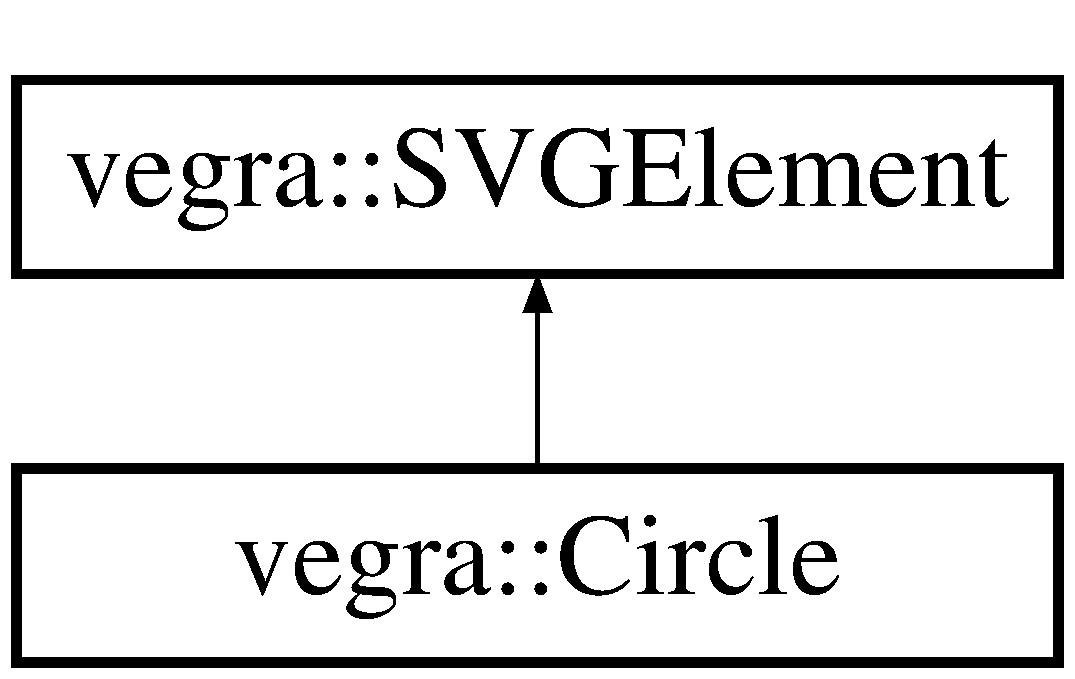
\includegraphics[height=2.000000cm]{structvegra_1_1Circle}
\end{center}
\end{figure}
\subsection*{Public Member Functions}
\begin{DoxyCompactItemize}
\item 
\mbox{\hyperlink{structvegra_1_1Circle_a30b817f23ffab115eda5d1d1a36d0a9b}{Circle}} ()
\item 
void \mbox{\hyperlink{structvegra_1_1Circle_adcfee7bc2183fb2173bc9a27659457bf}{add}} ()
\item 
void \mbox{\hyperlink{structvegra_1_1Circle_acf78b38e6f133931c4963652db3b382b}{add}} (\mbox{\hyperlink{structvegra_1_1SVGElement}{vegra\+::\+S\+V\+G\+Element}} $\ast$element)
\item 
{\footnotesize template$<$typename... Args$>$ }\\void \mbox{\hyperlink{structvegra_1_1Circle_a5e6f8b011ad3083ef2f3b8a731f96c7d}{add}} (\mbox{\hyperlink{structvegra_1_1SVGElement}{vegra\+::\+S\+V\+G\+Element}} $\ast$element, Args... args)
\item 
std\+::string \mbox{\hyperlink{structvegra_1_1Circle_ad32a663886487547c33ebeef6449c19a}{compose\+Element}} ()
\item 
void \mbox{\hyperlink{structvegra_1_1Circle_a67bfa48e7697a6ee3e7c79fed1129a3c}{wrap\+Element}} ()
\item 
void \mbox{\hyperlink{structvegra_1_1Circle_a25017785ce433a356b6b15b5d2d36060}{set\+Center}} (\mbox{\hyperlink{structvegra_1_1Center}{vegra\+::\+Center}} center)
\item 
void \mbox{\hyperlink{structvegra_1_1Circle_ac6f88039c6d3f666a8156876455854d0}{set\+Radius}} (\mbox{\hyperlink{structvegra_1_1Radius}{Radius}} radius)
\item 
void \mbox{\hyperlink{structvegra_1_1Circle_a85efa989ca99a6639fe24918b19c78b3}{set\+Stroke}} (\mbox{\hyperlink{structvegra_1_1Stroke}{vegra\+::\+Stroke}} stroke)
\item 
void \mbox{\hyperlink{structvegra_1_1Circle_a3a5d0f5879eb8ecba92782670dc386b4}{set\+Fill}} (\mbox{\hyperlink{structvegra_1_1Fill}{vegra\+::\+Fill}} fill)
\item 
\mbox{\hyperlink{namespacevegra_a2722f5eceb74f65746a02a57b71d125e}{S\+V\+G\+Element\+List}} \mbox{\hyperlink{structvegra_1_1Circle_a657b1849c50925b9f38e1f13ac0f4cd5}{get\+Elements}} ()
\begin{DoxyCompactList}\small\item\em Funtion to get svg element list. \end{DoxyCompactList}\item 
\mbox{\hyperlink{structvegra_1_1Center}{vegra\+::\+Center}} \mbox{\hyperlink{structvegra_1_1Circle_a8dd74def2123ae009053c067f653380d}{get\+Center}} ()
\item 
\mbox{\hyperlink{structvegra_1_1Radius}{vegra\+::\+Radius}} \mbox{\hyperlink{structvegra_1_1Circle_ad9eb941c53b548d6944e8d95f9ff1328}{get\+Radius}} ()
\item 
\mbox{\hyperlink{structvegra_1_1Stroke}{vegra\+::\+Stroke}} \mbox{\hyperlink{structvegra_1_1Circle_ab0ab83cb024a9b236c87194fdada9055}{get\+Stroke}} ()
\item 
\mbox{\hyperlink{structvegra_1_1Fill}{vegra\+::\+Fill}} \mbox{\hyperlink{structvegra_1_1Circle_a8f68bc2e3f0469a479d5314b81aeffc8}{get\+Fill}} ()
\item 
std\+::string \mbox{\hyperlink{structvegra_1_1Circle_a50bdbe7e4b29530b131e7a1157190b00}{get\+Element}} () override
\end{DoxyCompactItemize}


\subsection{Constructor \& Destructor Documentation}
\mbox{\Hypertarget{structvegra_1_1Circle_a30b817f23ffab115eda5d1d1a36d0a9b}\label{structvegra_1_1Circle_a30b817f23ffab115eda5d1d1a36d0a9b}} 
\index{vegra\+::\+Circle@{vegra\+::\+Circle}!Circle@{Circle}}
\index{Circle@{Circle}!vegra\+::\+Circle@{vegra\+::\+Circle}}
\subsubsection{\texorpdfstring{Circle()}{Circle()}}
{\footnotesize\ttfamily vegra\+::\+Circle\+::\+Circle (\begin{DoxyParamCaption}{ }\end{DoxyParamCaption})\hspace{0.3cm}{\ttfamily [inline]}}



\subsection{Member Function Documentation}
\mbox{\Hypertarget{structvegra_1_1Circle_adcfee7bc2183fb2173bc9a27659457bf}\label{structvegra_1_1Circle_adcfee7bc2183fb2173bc9a27659457bf}} 
\index{vegra\+::\+Circle@{vegra\+::\+Circle}!add@{add}}
\index{add@{add}!vegra\+::\+Circle@{vegra\+::\+Circle}}
\subsubsection{\texorpdfstring{add()}{add()}\hspace{0.1cm}{\footnotesize\ttfamily [1/3]}}
{\footnotesize\ttfamily void vegra\+::\+Circle\+::add (\begin{DoxyParamCaption}{ }\end{DoxyParamCaption})\hspace{0.3cm}{\ttfamily [inline]}}

\mbox{\Hypertarget{structvegra_1_1Circle_acf78b38e6f133931c4963652db3b382b}\label{structvegra_1_1Circle_acf78b38e6f133931c4963652db3b382b}} 
\index{vegra\+::\+Circle@{vegra\+::\+Circle}!add@{add}}
\index{add@{add}!vegra\+::\+Circle@{vegra\+::\+Circle}}
\subsubsection{\texorpdfstring{add()}{add()}\hspace{0.1cm}{\footnotesize\ttfamily [2/3]}}
{\footnotesize\ttfamily void vegra\+::\+Circle\+::add (\begin{DoxyParamCaption}\item[{\mbox{\hyperlink{structvegra_1_1SVGElement}{vegra\+::\+S\+V\+G\+Element}} $\ast$}]{element }\end{DoxyParamCaption})\hspace{0.3cm}{\ttfamily [inline]}}

\mbox{\Hypertarget{structvegra_1_1Circle_a5e6f8b011ad3083ef2f3b8a731f96c7d}\label{structvegra_1_1Circle_a5e6f8b011ad3083ef2f3b8a731f96c7d}} 
\index{vegra\+::\+Circle@{vegra\+::\+Circle}!add@{add}}
\index{add@{add}!vegra\+::\+Circle@{vegra\+::\+Circle}}
\subsubsection{\texorpdfstring{add()}{add()}\hspace{0.1cm}{\footnotesize\ttfamily [3/3]}}
{\footnotesize\ttfamily template$<$typename... Args$>$ \\
void vegra\+::\+Circle\+::add (\begin{DoxyParamCaption}\item[{\mbox{\hyperlink{structvegra_1_1SVGElement}{vegra\+::\+S\+V\+G\+Element}} $\ast$}]{element,  }\item[{Args...}]{args }\end{DoxyParamCaption})\hspace{0.3cm}{\ttfamily [inline]}}

\mbox{\Hypertarget{structvegra_1_1Circle_ad32a663886487547c33ebeef6449c19a}\label{structvegra_1_1Circle_ad32a663886487547c33ebeef6449c19a}} 
\index{vegra\+::\+Circle@{vegra\+::\+Circle}!compose\+Element@{compose\+Element}}
\index{compose\+Element@{compose\+Element}!vegra\+::\+Circle@{vegra\+::\+Circle}}
\subsubsection{\texorpdfstring{compose\+Element()}{composeElement()}}
{\footnotesize\ttfamily std\+::string vegra\+::\+Circle\+::compose\+Element (\begin{DoxyParamCaption}{ }\end{DoxyParamCaption})\hspace{0.3cm}{\ttfamily [inline]}}

\mbox{\Hypertarget{structvegra_1_1Circle_a8dd74def2123ae009053c067f653380d}\label{structvegra_1_1Circle_a8dd74def2123ae009053c067f653380d}} 
\index{vegra\+::\+Circle@{vegra\+::\+Circle}!get\+Center@{get\+Center}}
\index{get\+Center@{get\+Center}!vegra\+::\+Circle@{vegra\+::\+Circle}}
\subsubsection{\texorpdfstring{get\+Center()}{getCenter()}}
{\footnotesize\ttfamily \mbox{\hyperlink{structvegra_1_1Center}{vegra\+::\+Center}} vegra\+::\+Circle\+::get\+Center (\begin{DoxyParamCaption}{ }\end{DoxyParamCaption})\hspace{0.3cm}{\ttfamily [inline]}}

\mbox{\Hypertarget{structvegra_1_1Circle_a50bdbe7e4b29530b131e7a1157190b00}\label{structvegra_1_1Circle_a50bdbe7e4b29530b131e7a1157190b00}} 
\index{vegra\+::\+Circle@{vegra\+::\+Circle}!get\+Element@{get\+Element}}
\index{get\+Element@{get\+Element}!vegra\+::\+Circle@{vegra\+::\+Circle}}
\subsubsection{\texorpdfstring{get\+Element()}{getElement()}}
{\footnotesize\ttfamily std\+::string vegra\+::\+Circle\+::get\+Element (\begin{DoxyParamCaption}{ }\end{DoxyParamCaption})\hspace{0.3cm}{\ttfamily [inline]}, {\ttfamily [override]}, {\ttfamily [virtual]}}



Implements \mbox{\hyperlink{structvegra_1_1SVGElement_a17fa30b9de97e1541eaa1f6888145de2}{vegra\+::\+S\+V\+G\+Element}}.

\mbox{\Hypertarget{structvegra_1_1Circle_a657b1849c50925b9f38e1f13ac0f4cd5}\label{structvegra_1_1Circle_a657b1849c50925b9f38e1f13ac0f4cd5}} 
\index{vegra\+::\+Circle@{vegra\+::\+Circle}!get\+Elements@{get\+Elements}}
\index{get\+Elements@{get\+Elements}!vegra\+::\+Circle@{vegra\+::\+Circle}}
\subsubsection{\texorpdfstring{get\+Elements()}{getElements()}}
{\footnotesize\ttfamily \mbox{\hyperlink{namespacevegra_a2722f5eceb74f65746a02a57b71d125e}{S\+V\+G\+Element\+List}} vegra\+::\+Circle\+::get\+Elements (\begin{DoxyParamCaption}{ }\end{DoxyParamCaption})\hspace{0.3cm}{\ttfamily [inline]}}



Funtion to get svg element list. 

\mbox{\Hypertarget{structvegra_1_1Circle_a8f68bc2e3f0469a479d5314b81aeffc8}\label{structvegra_1_1Circle_a8f68bc2e3f0469a479d5314b81aeffc8}} 
\index{vegra\+::\+Circle@{vegra\+::\+Circle}!get\+Fill@{get\+Fill}}
\index{get\+Fill@{get\+Fill}!vegra\+::\+Circle@{vegra\+::\+Circle}}
\subsubsection{\texorpdfstring{get\+Fill()}{getFill()}}
{\footnotesize\ttfamily \mbox{\hyperlink{structvegra_1_1Fill}{vegra\+::\+Fill}} vegra\+::\+Circle\+::get\+Fill (\begin{DoxyParamCaption}{ }\end{DoxyParamCaption})\hspace{0.3cm}{\ttfamily [inline]}}

\mbox{\Hypertarget{structvegra_1_1Circle_ad9eb941c53b548d6944e8d95f9ff1328}\label{structvegra_1_1Circle_ad9eb941c53b548d6944e8d95f9ff1328}} 
\index{vegra\+::\+Circle@{vegra\+::\+Circle}!get\+Radius@{get\+Radius}}
\index{get\+Radius@{get\+Radius}!vegra\+::\+Circle@{vegra\+::\+Circle}}
\subsubsection{\texorpdfstring{get\+Radius()}{getRadius()}}
{\footnotesize\ttfamily \mbox{\hyperlink{structvegra_1_1Radius}{vegra\+::\+Radius}} vegra\+::\+Circle\+::get\+Radius (\begin{DoxyParamCaption}{ }\end{DoxyParamCaption})\hspace{0.3cm}{\ttfamily [inline]}}

\mbox{\Hypertarget{structvegra_1_1Circle_ab0ab83cb024a9b236c87194fdada9055}\label{structvegra_1_1Circle_ab0ab83cb024a9b236c87194fdada9055}} 
\index{vegra\+::\+Circle@{vegra\+::\+Circle}!get\+Stroke@{get\+Stroke}}
\index{get\+Stroke@{get\+Stroke}!vegra\+::\+Circle@{vegra\+::\+Circle}}
\subsubsection{\texorpdfstring{get\+Stroke()}{getStroke()}}
{\footnotesize\ttfamily \mbox{\hyperlink{structvegra_1_1Stroke}{vegra\+::\+Stroke}} vegra\+::\+Circle\+::get\+Stroke (\begin{DoxyParamCaption}{ }\end{DoxyParamCaption})\hspace{0.3cm}{\ttfamily [inline]}}

\mbox{\Hypertarget{structvegra_1_1Circle_a25017785ce433a356b6b15b5d2d36060}\label{structvegra_1_1Circle_a25017785ce433a356b6b15b5d2d36060}} 
\index{vegra\+::\+Circle@{vegra\+::\+Circle}!set\+Center@{set\+Center}}
\index{set\+Center@{set\+Center}!vegra\+::\+Circle@{vegra\+::\+Circle}}
\subsubsection{\texorpdfstring{set\+Center()}{setCenter()}}
{\footnotesize\ttfamily void vegra\+::\+Circle\+::set\+Center (\begin{DoxyParamCaption}\item[{\mbox{\hyperlink{structvegra_1_1Center}{vegra\+::\+Center}}}]{center }\end{DoxyParamCaption})\hspace{0.3cm}{\ttfamily [inline]}}

\mbox{\Hypertarget{structvegra_1_1Circle_a3a5d0f5879eb8ecba92782670dc386b4}\label{structvegra_1_1Circle_a3a5d0f5879eb8ecba92782670dc386b4}} 
\index{vegra\+::\+Circle@{vegra\+::\+Circle}!set\+Fill@{set\+Fill}}
\index{set\+Fill@{set\+Fill}!vegra\+::\+Circle@{vegra\+::\+Circle}}
\subsubsection{\texorpdfstring{set\+Fill()}{setFill()}}
{\footnotesize\ttfamily void vegra\+::\+Circle\+::set\+Fill (\begin{DoxyParamCaption}\item[{\mbox{\hyperlink{structvegra_1_1Fill}{vegra\+::\+Fill}}}]{fill }\end{DoxyParamCaption})\hspace{0.3cm}{\ttfamily [inline]}}

\mbox{\Hypertarget{structvegra_1_1Circle_ac6f88039c6d3f666a8156876455854d0}\label{structvegra_1_1Circle_ac6f88039c6d3f666a8156876455854d0}} 
\index{vegra\+::\+Circle@{vegra\+::\+Circle}!set\+Radius@{set\+Radius}}
\index{set\+Radius@{set\+Radius}!vegra\+::\+Circle@{vegra\+::\+Circle}}
\subsubsection{\texorpdfstring{set\+Radius()}{setRadius()}}
{\footnotesize\ttfamily void vegra\+::\+Circle\+::set\+Radius (\begin{DoxyParamCaption}\item[{\mbox{\hyperlink{structvegra_1_1Radius}{Radius}}}]{radius }\end{DoxyParamCaption})\hspace{0.3cm}{\ttfamily [inline]}}

\mbox{\Hypertarget{structvegra_1_1Circle_a85efa989ca99a6639fe24918b19c78b3}\label{structvegra_1_1Circle_a85efa989ca99a6639fe24918b19c78b3}} 
\index{vegra\+::\+Circle@{vegra\+::\+Circle}!set\+Stroke@{set\+Stroke}}
\index{set\+Stroke@{set\+Stroke}!vegra\+::\+Circle@{vegra\+::\+Circle}}
\subsubsection{\texorpdfstring{set\+Stroke()}{setStroke()}}
{\footnotesize\ttfamily void vegra\+::\+Circle\+::set\+Stroke (\begin{DoxyParamCaption}\item[{\mbox{\hyperlink{structvegra_1_1Stroke}{vegra\+::\+Stroke}}}]{stroke }\end{DoxyParamCaption})\hspace{0.3cm}{\ttfamily [inline]}}

\mbox{\Hypertarget{structvegra_1_1Circle_a67bfa48e7697a6ee3e7c79fed1129a3c}\label{structvegra_1_1Circle_a67bfa48e7697a6ee3e7c79fed1129a3c}} 
\index{vegra\+::\+Circle@{vegra\+::\+Circle}!wrap\+Element@{wrap\+Element}}
\index{wrap\+Element@{wrap\+Element}!vegra\+::\+Circle@{vegra\+::\+Circle}}
\subsubsection{\texorpdfstring{wrap\+Element()}{wrapElement()}}
{\footnotesize\ttfamily void vegra\+::\+Circle\+::wrap\+Element (\begin{DoxyParamCaption}{ }\end{DoxyParamCaption})\hspace{0.3cm}{\ttfamily [inline]}, {\ttfamily [virtual]}}



Implements \mbox{\hyperlink{structvegra_1_1SVGElement_a1369400ebe57287f1b5beb5f0234d8d7}{vegra\+::\+S\+V\+G\+Element}}.



The documentation for this struct was generated from the following file\+:\begin{DoxyCompactItemize}
\item 
/home/raghu/\+Development/vegra/include/\mbox{\hyperlink{circle_8h}{circle.\+h}}\end{DoxyCompactItemize}

\hypertarget{structvegra_1_1Fill}{}\section{vegra\+:\+:Fill Struct Reference}
\label{structvegra_1_1Fill}\index{vegra\+::\+Fill@{vegra\+::\+Fill}}


Attribute control fill inside the svg element.  




{\ttfamily \#include $<$attrib.\+h$>$}

\subsection*{Public Member Functions}
\begin{DoxyCompactItemize}
\item 
\mbox{\hyperlink{structvegra_1_1Fill_aa305a257a120bc2f164853ff5b4f8372}{Fill}} ()
\item 
\mbox{\hyperlink{structvegra_1_1Fill_abcf0ef6c4fcf15ba55f3c3ec576dc550}{Fill}} (std\+::string \mbox{\hyperlink{structvegra_1_1Fill_a04e027e6c024853598f4f1f9750a18f5}{color}}, double \mbox{\hyperlink{structvegra_1_1Fill_a19afcc63bea86ccbb0eb425ca8ba3648}{opacity}})
\item 
void \mbox{\hyperlink{structvegra_1_1Fill_ab05e35510d4dfec3455cb537ab5bc227}{set\+Color}} (std\+::string \mbox{\hyperlink{structvegra_1_1Fill_a04e027e6c024853598f4f1f9750a18f5}{color}})
\item 
void \mbox{\hyperlink{structvegra_1_1Fill_a4968a0a2cb88537a0ea6aaf6bf095ad5}{set\+Opacity}} (double \mbox{\hyperlink{structvegra_1_1Fill_a19afcc63bea86ccbb0eb425ca8ba3648}{opacity}})
\item 
std\+::string \mbox{\hyperlink{structvegra_1_1Fill_a2dddee85ed5bf8e6455af59e69ef0dc8}{get\+Color}} ()
\item 
double \mbox{\hyperlink{structvegra_1_1Fill_a53203023282b847dec9aa3bf55507cde}{get\+Opacity}} ()
\end{DoxyCompactItemize}
\subsection*{Public Attributes}
\begin{DoxyCompactItemize}
\item 
std\+::string \mbox{\hyperlink{structvegra_1_1Fill_a04e027e6c024853598f4f1f9750a18f5}{color}}
\item 
double \mbox{\hyperlink{structvegra_1_1Fill_a19afcc63bea86ccbb0eb425ca8ba3648}{opacity}}
\begin{DoxyCompactList}\small\item\em fill \end{DoxyCompactList}\end{DoxyCompactItemize}


\subsection{Detailed Description}
Attribute control fill inside the svg element. 

\subsection{Constructor \& Destructor Documentation}
\mbox{\Hypertarget{structvegra_1_1Fill_aa305a257a120bc2f164853ff5b4f8372}\label{structvegra_1_1Fill_aa305a257a120bc2f164853ff5b4f8372}} 
\index{vegra\+::\+Fill@{vegra\+::\+Fill}!Fill@{Fill}}
\index{Fill@{Fill}!vegra\+::\+Fill@{vegra\+::\+Fill}}
\subsubsection{\texorpdfstring{Fill()}{Fill()}\hspace{0.1cm}{\footnotesize\ttfamily [1/2]}}
{\footnotesize\ttfamily vegra\+::\+Fill\+::\+Fill (\begin{DoxyParamCaption}{ }\end{DoxyParamCaption})\hspace{0.3cm}{\ttfamily [inline]}}

\mbox{\Hypertarget{structvegra_1_1Fill_abcf0ef6c4fcf15ba55f3c3ec576dc550}\label{structvegra_1_1Fill_abcf0ef6c4fcf15ba55f3c3ec576dc550}} 
\index{vegra\+::\+Fill@{vegra\+::\+Fill}!Fill@{Fill}}
\index{Fill@{Fill}!vegra\+::\+Fill@{vegra\+::\+Fill}}
\subsubsection{\texorpdfstring{Fill()}{Fill()}\hspace{0.1cm}{\footnotesize\ttfamily [2/2]}}
{\footnotesize\ttfamily vegra\+::\+Fill\+::\+Fill (\begin{DoxyParamCaption}\item[{std\+::string}]{color,  }\item[{double}]{opacity }\end{DoxyParamCaption})\hspace{0.3cm}{\ttfamily [inline]}}



\subsection{Member Function Documentation}
\mbox{\Hypertarget{structvegra_1_1Fill_a2dddee85ed5bf8e6455af59e69ef0dc8}\label{structvegra_1_1Fill_a2dddee85ed5bf8e6455af59e69ef0dc8}} 
\index{vegra\+::\+Fill@{vegra\+::\+Fill}!get\+Color@{get\+Color}}
\index{get\+Color@{get\+Color}!vegra\+::\+Fill@{vegra\+::\+Fill}}
\subsubsection{\texorpdfstring{get\+Color()}{getColor()}}
{\footnotesize\ttfamily std\+::string vegra\+::\+Fill\+::get\+Color (\begin{DoxyParamCaption}{ }\end{DoxyParamCaption})\hspace{0.3cm}{\ttfamily [inline]}}

\mbox{\Hypertarget{structvegra_1_1Fill_a53203023282b847dec9aa3bf55507cde}\label{structvegra_1_1Fill_a53203023282b847dec9aa3bf55507cde}} 
\index{vegra\+::\+Fill@{vegra\+::\+Fill}!get\+Opacity@{get\+Opacity}}
\index{get\+Opacity@{get\+Opacity}!vegra\+::\+Fill@{vegra\+::\+Fill}}
\subsubsection{\texorpdfstring{get\+Opacity()}{getOpacity()}}
{\footnotesize\ttfamily double vegra\+::\+Fill\+::get\+Opacity (\begin{DoxyParamCaption}{ }\end{DoxyParamCaption})\hspace{0.3cm}{\ttfamily [inline]}}

\mbox{\Hypertarget{structvegra_1_1Fill_ab05e35510d4dfec3455cb537ab5bc227}\label{structvegra_1_1Fill_ab05e35510d4dfec3455cb537ab5bc227}} 
\index{vegra\+::\+Fill@{vegra\+::\+Fill}!set\+Color@{set\+Color}}
\index{set\+Color@{set\+Color}!vegra\+::\+Fill@{vegra\+::\+Fill}}
\subsubsection{\texorpdfstring{set\+Color()}{setColor()}}
{\footnotesize\ttfamily void vegra\+::\+Fill\+::set\+Color (\begin{DoxyParamCaption}\item[{std\+::string}]{color }\end{DoxyParamCaption})\hspace{0.3cm}{\ttfamily [inline]}}

\mbox{\Hypertarget{structvegra_1_1Fill_a4968a0a2cb88537a0ea6aaf6bf095ad5}\label{structvegra_1_1Fill_a4968a0a2cb88537a0ea6aaf6bf095ad5}} 
\index{vegra\+::\+Fill@{vegra\+::\+Fill}!set\+Opacity@{set\+Opacity}}
\index{set\+Opacity@{set\+Opacity}!vegra\+::\+Fill@{vegra\+::\+Fill}}
\subsubsection{\texorpdfstring{set\+Opacity()}{setOpacity()}}
{\footnotesize\ttfamily void vegra\+::\+Fill\+::set\+Opacity (\begin{DoxyParamCaption}\item[{double}]{opacity }\end{DoxyParamCaption})\hspace{0.3cm}{\ttfamily [inline]}}



\subsection{Member Data Documentation}
\mbox{\Hypertarget{structvegra_1_1Fill_a04e027e6c024853598f4f1f9750a18f5}\label{structvegra_1_1Fill_a04e027e6c024853598f4f1f9750a18f5}} 
\index{vegra\+::\+Fill@{vegra\+::\+Fill}!color@{color}}
\index{color@{color}!vegra\+::\+Fill@{vegra\+::\+Fill}}
\subsubsection{\texorpdfstring{color}{color}}
{\footnotesize\ttfamily std\+::string vegra\+::\+Fill\+::color}

\mbox{\Hypertarget{structvegra_1_1Fill_a19afcc63bea86ccbb0eb425ca8ba3648}\label{structvegra_1_1Fill_a19afcc63bea86ccbb0eb425ca8ba3648}} 
\index{vegra\+::\+Fill@{vegra\+::\+Fill}!opacity@{opacity}}
\index{opacity@{opacity}!vegra\+::\+Fill@{vegra\+::\+Fill}}
\subsubsection{\texorpdfstring{opacity}{opacity}}
{\footnotesize\ttfamily double vegra\+::\+Fill\+::opacity}



fill 



The documentation for this struct was generated from the following file\+:\begin{DoxyCompactItemize}
\item 
/home/raghu/\+Development/vegra/include/\mbox{\hyperlink{attrib_8h}{attrib.\+h}}\end{DoxyCompactItemize}

\hypertarget{structvegra_1_1InvalidAttribException}{}\section{vegra\+:\+:Invalid\+Attrib\+Exception Struct Reference}
\label{structvegra_1_1InvalidAttribException}\index{vegra\+::\+Invalid\+Attrib\+Exception@{vegra\+::\+Invalid\+Attrib\+Exception}}


Invalid attrib exception -\/ Throw when invalid attribute is passed to a function.  




{\ttfamily \#include $<$exception.\+h$>$}

Inheritance diagram for vegra\+:\+:Invalid\+Attrib\+Exception\+:\begin{figure}[H]
\begin{center}
\leavevmode
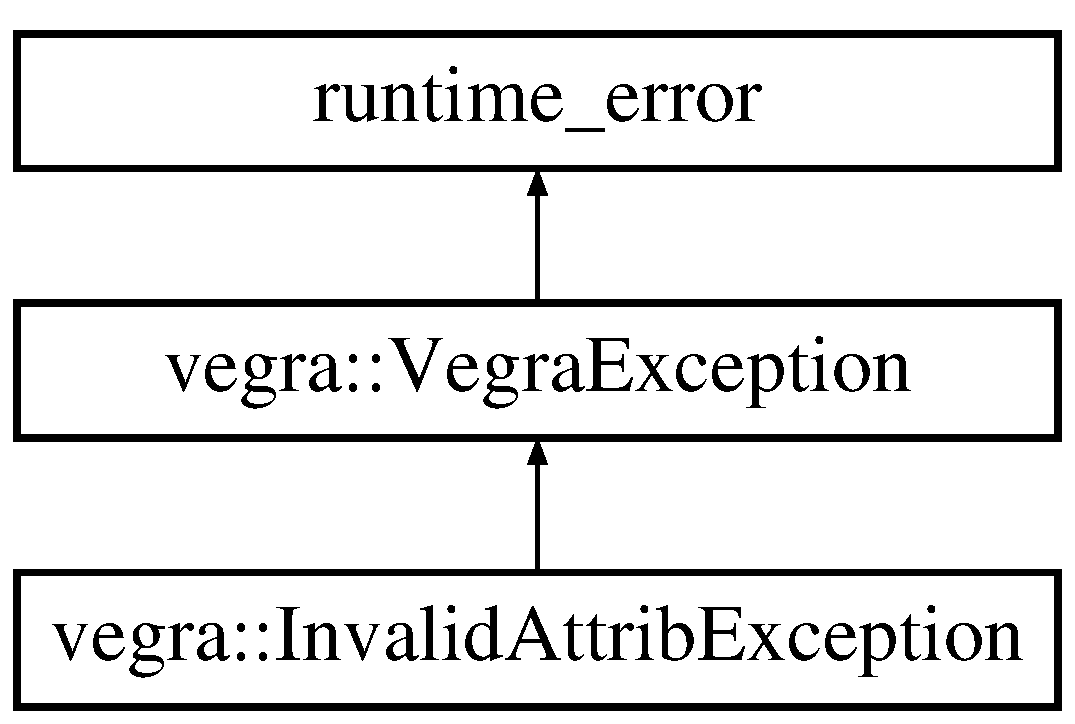
\includegraphics[height=3.000000cm]{structvegra_1_1InvalidAttribException}
\end{center}
\end{figure}
\subsection*{Public Member Functions}
\begin{DoxyCompactItemize}
\item 
\mbox{\hyperlink{structvegra_1_1InvalidAttribException_a919670428f8052ce5814b9665d6d9838}{Invalid\+Attrib\+Exception}} (const std\+::string \&msg)
\end{DoxyCompactItemize}


\subsection{Detailed Description}
Invalid attrib exception -\/ Throw when invalid attribute is passed to a function. 

\subsection{Constructor \& Destructor Documentation}
\mbox{\Hypertarget{structvegra_1_1InvalidAttribException_a919670428f8052ce5814b9665d6d9838}\label{structvegra_1_1InvalidAttribException_a919670428f8052ce5814b9665d6d9838}} 
\index{vegra\+::\+Invalid\+Attrib\+Exception@{vegra\+::\+Invalid\+Attrib\+Exception}!Invalid\+Attrib\+Exception@{Invalid\+Attrib\+Exception}}
\index{Invalid\+Attrib\+Exception@{Invalid\+Attrib\+Exception}!vegra\+::\+Invalid\+Attrib\+Exception@{vegra\+::\+Invalid\+Attrib\+Exception}}
\subsubsection{\texorpdfstring{Invalid\+Attrib\+Exception()}{InvalidAttribException()}}
{\footnotesize\ttfamily vegra\+::\+Invalid\+Attrib\+Exception\+::\+Invalid\+Attrib\+Exception (\begin{DoxyParamCaption}\item[{const std\+::string \&}]{msg }\end{DoxyParamCaption})\hspace{0.3cm}{\ttfamily [inline]}, {\ttfamily [explicit]}}



The documentation for this struct was generated from the following file\+:\begin{DoxyCompactItemize}
\item 
/home/raghu/\+Development/vegra/include/\mbox{\hyperlink{exception_8h}{exception.\+h}}\end{DoxyCompactItemize}

\hypertarget{structvegra_1_1InvalidParamException}{}\section{vegra\+:\+:Invalid\+Param\+Exception Struct Reference}
\label{structvegra_1_1InvalidParamException}\index{vegra\+::\+Invalid\+Param\+Exception@{vegra\+::\+Invalid\+Param\+Exception}}


{\ttfamily \#include $<$exception.\+h$>$}

Inheritance diagram for vegra\+:\+:Invalid\+Param\+Exception\+:\begin{figure}[H]
\begin{center}
\leavevmode
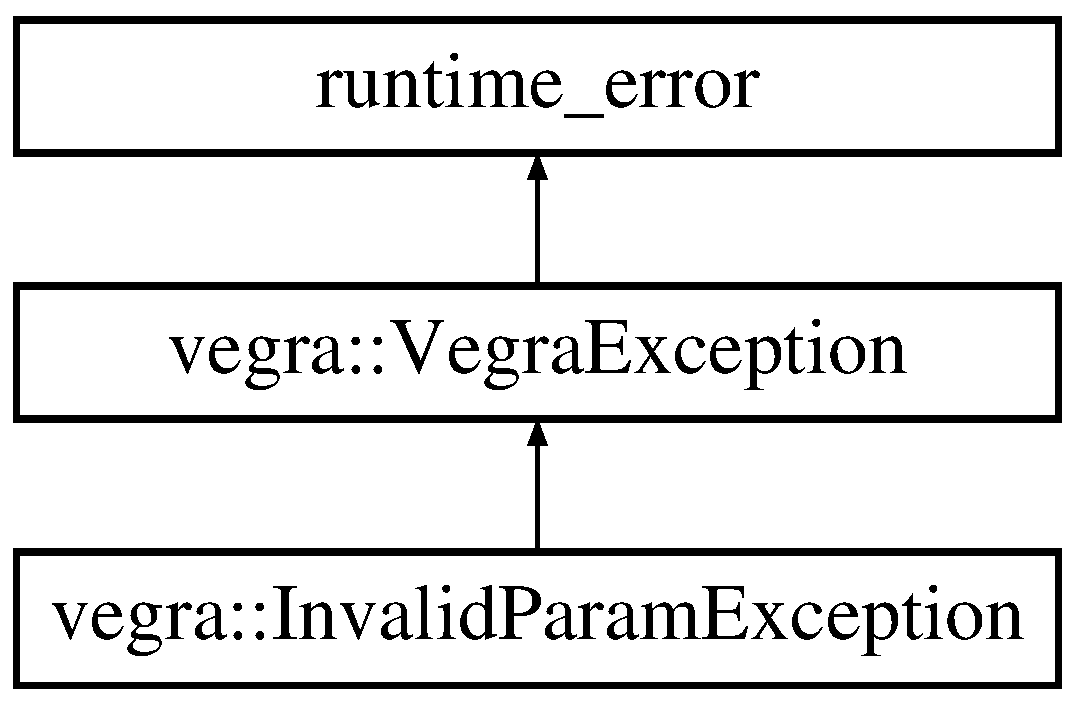
\includegraphics[height=3.000000cm]{structvegra_1_1InvalidParamException}
\end{center}
\end{figure}
\subsection*{Public Member Functions}
\begin{DoxyCompactItemize}
\item 
\mbox{\hyperlink{structvegra_1_1InvalidParamException_a53ef0c110a6dbcfacf38870798dafba5}{Invalid\+Param\+Exception}} (const std\+::string \&msg)
\end{DoxyCompactItemize}


\subsection{Constructor \& Destructor Documentation}
\mbox{\Hypertarget{structvegra_1_1InvalidParamException_a53ef0c110a6dbcfacf38870798dafba5}\label{structvegra_1_1InvalidParamException_a53ef0c110a6dbcfacf38870798dafba5}} 
\index{vegra\+::\+Invalid\+Param\+Exception@{vegra\+::\+Invalid\+Param\+Exception}!Invalid\+Param\+Exception@{Invalid\+Param\+Exception}}
\index{Invalid\+Param\+Exception@{Invalid\+Param\+Exception}!vegra\+::\+Invalid\+Param\+Exception@{vegra\+::\+Invalid\+Param\+Exception}}
\subsubsection{\texorpdfstring{Invalid\+Param\+Exception()}{InvalidParamException()}}
{\footnotesize\ttfamily vegra\+::\+Invalid\+Param\+Exception\+::\+Invalid\+Param\+Exception (\begin{DoxyParamCaption}\item[{const std\+::string \&}]{msg }\end{DoxyParamCaption})\hspace{0.3cm}{\ttfamily [inline]}, {\ttfamily [explicit]}}



The documentation for this struct was generated from the following file\+:\begin{DoxyCompactItemize}
\item 
/home/raghu/\+Development/vegra/include/\mbox{\hyperlink{exception_8h}{exception.\+h}}\end{DoxyCompactItemize}

\hypertarget{structvegra_1_1InvalidTypeException}{}\section{vegra\+:\+:Invalid\+Type\+Exception Struct Reference}
\label{structvegra_1_1InvalidTypeException}\index{vegra\+::\+Invalid\+Type\+Exception@{vegra\+::\+Invalid\+Type\+Exception}}


Invalid Type Exception -\/ Throw when a non svg type is passed.  




{\ttfamily \#include $<$exception.\+h$>$}

Inheritance diagram for vegra\+:\+:Invalid\+Type\+Exception\+:\begin{figure}[H]
\begin{center}
\leavevmode
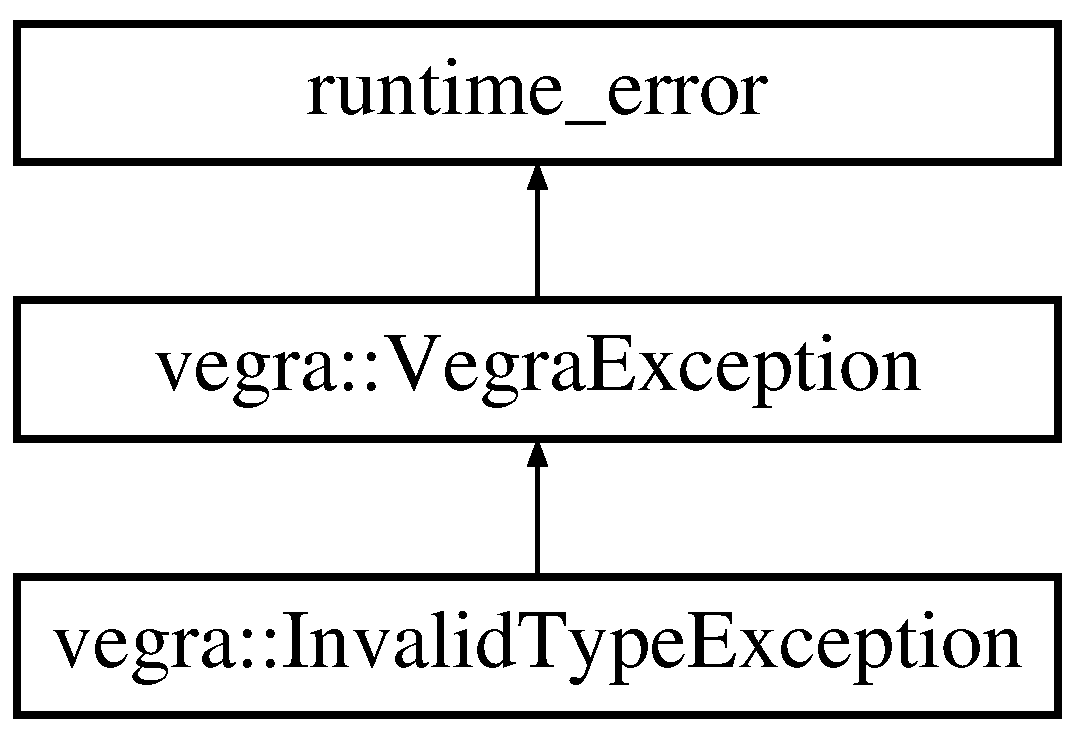
\includegraphics[height=3.000000cm]{structvegra_1_1InvalidTypeException}
\end{center}
\end{figure}
\subsection*{Public Member Functions}
\begin{DoxyCompactItemize}
\item 
\mbox{\hyperlink{structvegra_1_1InvalidTypeException_a302b895279c85376f3370a6734b029f5}{Invalid\+Type\+Exception}} (const std\+::string \&msg)
\end{DoxyCompactItemize}


\subsection{Detailed Description}
Invalid Type Exception -\/ Throw when a non svg type is passed. 

\subsection{Constructor \& Destructor Documentation}
\mbox{\Hypertarget{structvegra_1_1InvalidTypeException_a302b895279c85376f3370a6734b029f5}\label{structvegra_1_1InvalidTypeException_a302b895279c85376f3370a6734b029f5}} 
\index{vegra\+::\+Invalid\+Type\+Exception@{vegra\+::\+Invalid\+Type\+Exception}!Invalid\+Type\+Exception@{Invalid\+Type\+Exception}}
\index{Invalid\+Type\+Exception@{Invalid\+Type\+Exception}!vegra\+::\+Invalid\+Type\+Exception@{vegra\+::\+Invalid\+Type\+Exception}}
\subsubsection{\texorpdfstring{Invalid\+Type\+Exception()}{InvalidTypeException()}}
{\footnotesize\ttfamily vegra\+::\+Invalid\+Type\+Exception\+::\+Invalid\+Type\+Exception (\begin{DoxyParamCaption}\item[{const std\+::string \&}]{msg }\end{DoxyParamCaption})\hspace{0.3cm}{\ttfamily [inline]}, {\ttfamily [explicit]}}



The documentation for this struct was generated from the following file\+:\begin{DoxyCompactItemize}
\item 
/home/raghu/\+Development/vegra/include/\mbox{\hyperlink{exception_8h}{exception.\+h}}\end{DoxyCompactItemize}

\hypertarget{structvegra_1_1Position}{}\section{vegra\+:\+:Position Struct Reference}
\label{structvegra_1_1Position}\index{vegra\+::\+Position@{vegra\+::\+Position}}


{\ttfamily \#include $<$attrib.\+h$>$}

\subsection*{Public Member Functions}
\begin{DoxyCompactItemize}
\item 
\mbox{\hyperlink{structvegra_1_1Position_af937e1b394be37468bff14e58a3e4156}{Position}} ()
\item 
\mbox{\hyperlink{structvegra_1_1Position_acafc039da99be520366e838103022c0b}{Position}} (int \mbox{\hyperlink{structvegra_1_1Position_a458595c84391b5ae3bdc0c8d256706b6}{x}}, int \mbox{\hyperlink{structvegra_1_1Position_a2e90d89fd65b914fe6b6157c2d20d90c}{y}})
\item 
void \mbox{\hyperlink{structvegra_1_1Position_a6f5f33e280592cce1670b9558d24d8a8}{set\+Position}} (int \mbox{\hyperlink{structvegra_1_1Position_a458595c84391b5ae3bdc0c8d256706b6}{x}}, int \mbox{\hyperlink{structvegra_1_1Position_a2e90d89fd65b914fe6b6157c2d20d90c}{y}})
\item 
void \mbox{\hyperlink{structvegra_1_1Position_a2accdc2782f0a67a529633c2c2125fe7}{setX}} (int \mbox{\hyperlink{structvegra_1_1Position_a458595c84391b5ae3bdc0c8d256706b6}{x}})
\item 
void \mbox{\hyperlink{structvegra_1_1Position_a1930518a71651b723688490e3adbe196}{setY}} (int \mbox{\hyperlink{structvegra_1_1Position_a2e90d89fd65b914fe6b6157c2d20d90c}{y}})
\item 
int \mbox{\hyperlink{structvegra_1_1Position_a5c93cf166315938b531e879ad31cddd1}{getX}} ()
\item 
int \mbox{\hyperlink{structvegra_1_1Position_a4580e90a19e9b28d4abc6a67326dce7a}{getY}} ()
\item 
\mbox{\hyperlink{structvegra_1_1Position}{Position}} \mbox{\hyperlink{structvegra_1_1Position_ab62133cb12f5886577670ba8623b5e09}{get\+Position}} ()
\end{DoxyCompactItemize}
\subsection*{Public Attributes}
\begin{DoxyCompactItemize}
\item 
int \mbox{\hyperlink{structvegra_1_1Position_a458595c84391b5ae3bdc0c8d256706b6}{x}}
\item 
int \mbox{\hyperlink{structvegra_1_1Position_a2e90d89fd65b914fe6b6157c2d20d90c}{y}}
\end{DoxyCompactItemize}


\subsection{Constructor \& Destructor Documentation}
\mbox{\Hypertarget{structvegra_1_1Position_af937e1b394be37468bff14e58a3e4156}\label{structvegra_1_1Position_af937e1b394be37468bff14e58a3e4156}} 
\index{vegra\+::\+Position@{vegra\+::\+Position}!Position@{Position}}
\index{Position@{Position}!vegra\+::\+Position@{vegra\+::\+Position}}
\subsubsection{\texorpdfstring{Position()}{Position()}\hspace{0.1cm}{\footnotesize\ttfamily [1/2]}}
{\footnotesize\ttfamily vegra\+::\+Position\+::\+Position (\begin{DoxyParamCaption}{ }\end{DoxyParamCaption})\hspace{0.3cm}{\ttfamily [inline]}}

\mbox{\Hypertarget{structvegra_1_1Position_acafc039da99be520366e838103022c0b}\label{structvegra_1_1Position_acafc039da99be520366e838103022c0b}} 
\index{vegra\+::\+Position@{vegra\+::\+Position}!Position@{Position}}
\index{Position@{Position}!vegra\+::\+Position@{vegra\+::\+Position}}
\subsubsection{\texorpdfstring{Position()}{Position()}\hspace{0.1cm}{\footnotesize\ttfamily [2/2]}}
{\footnotesize\ttfamily vegra\+::\+Position\+::\+Position (\begin{DoxyParamCaption}\item[{int}]{x,  }\item[{int}]{y }\end{DoxyParamCaption})\hspace{0.3cm}{\ttfamily [inline]}}



\subsection{Member Function Documentation}
\mbox{\Hypertarget{structvegra_1_1Position_ab62133cb12f5886577670ba8623b5e09}\label{structvegra_1_1Position_ab62133cb12f5886577670ba8623b5e09}} 
\index{vegra\+::\+Position@{vegra\+::\+Position}!get\+Position@{get\+Position}}
\index{get\+Position@{get\+Position}!vegra\+::\+Position@{vegra\+::\+Position}}
\subsubsection{\texorpdfstring{get\+Position()}{getPosition()}}
{\footnotesize\ttfamily \mbox{\hyperlink{structvegra_1_1Position}{Position}} vegra\+::\+Position\+::get\+Position (\begin{DoxyParamCaption}{ }\end{DoxyParamCaption})\hspace{0.3cm}{\ttfamily [inline]}}

\mbox{\Hypertarget{structvegra_1_1Position_a5c93cf166315938b531e879ad31cddd1}\label{structvegra_1_1Position_a5c93cf166315938b531e879ad31cddd1}} 
\index{vegra\+::\+Position@{vegra\+::\+Position}!getX@{getX}}
\index{getX@{getX}!vegra\+::\+Position@{vegra\+::\+Position}}
\subsubsection{\texorpdfstring{get\+X()}{getX()}}
{\footnotesize\ttfamily int vegra\+::\+Position\+::getX (\begin{DoxyParamCaption}{ }\end{DoxyParamCaption})\hspace{0.3cm}{\ttfamily [inline]}}

\mbox{\Hypertarget{structvegra_1_1Position_a4580e90a19e9b28d4abc6a67326dce7a}\label{structvegra_1_1Position_a4580e90a19e9b28d4abc6a67326dce7a}} 
\index{vegra\+::\+Position@{vegra\+::\+Position}!getY@{getY}}
\index{getY@{getY}!vegra\+::\+Position@{vegra\+::\+Position}}
\subsubsection{\texorpdfstring{get\+Y()}{getY()}}
{\footnotesize\ttfamily int vegra\+::\+Position\+::getY (\begin{DoxyParamCaption}{ }\end{DoxyParamCaption})\hspace{0.3cm}{\ttfamily [inline]}}

\mbox{\Hypertarget{structvegra_1_1Position_a6f5f33e280592cce1670b9558d24d8a8}\label{structvegra_1_1Position_a6f5f33e280592cce1670b9558d24d8a8}} 
\index{vegra\+::\+Position@{vegra\+::\+Position}!set\+Position@{set\+Position}}
\index{set\+Position@{set\+Position}!vegra\+::\+Position@{vegra\+::\+Position}}
\subsubsection{\texorpdfstring{set\+Position()}{setPosition()}}
{\footnotesize\ttfamily void vegra\+::\+Position\+::set\+Position (\begin{DoxyParamCaption}\item[{int}]{x,  }\item[{int}]{y }\end{DoxyParamCaption})\hspace{0.3cm}{\ttfamily [inline]}}

\mbox{\Hypertarget{structvegra_1_1Position_a2accdc2782f0a67a529633c2c2125fe7}\label{structvegra_1_1Position_a2accdc2782f0a67a529633c2c2125fe7}} 
\index{vegra\+::\+Position@{vegra\+::\+Position}!setX@{setX}}
\index{setX@{setX}!vegra\+::\+Position@{vegra\+::\+Position}}
\subsubsection{\texorpdfstring{set\+X()}{setX()}}
{\footnotesize\ttfamily void vegra\+::\+Position\+::setX (\begin{DoxyParamCaption}\item[{int}]{x }\end{DoxyParamCaption})\hspace{0.3cm}{\ttfamily [inline]}}

\mbox{\Hypertarget{structvegra_1_1Position_a1930518a71651b723688490e3adbe196}\label{structvegra_1_1Position_a1930518a71651b723688490e3adbe196}} 
\index{vegra\+::\+Position@{vegra\+::\+Position}!setY@{setY}}
\index{setY@{setY}!vegra\+::\+Position@{vegra\+::\+Position}}
\subsubsection{\texorpdfstring{set\+Y()}{setY()}}
{\footnotesize\ttfamily void vegra\+::\+Position\+::setY (\begin{DoxyParamCaption}\item[{int}]{y }\end{DoxyParamCaption})\hspace{0.3cm}{\ttfamily [inline]}}



\subsection{Member Data Documentation}
\mbox{\Hypertarget{structvegra_1_1Position_a458595c84391b5ae3bdc0c8d256706b6}\label{structvegra_1_1Position_a458595c84391b5ae3bdc0c8d256706b6}} 
\index{vegra\+::\+Position@{vegra\+::\+Position}!x@{x}}
\index{x@{x}!vegra\+::\+Position@{vegra\+::\+Position}}
\subsubsection{\texorpdfstring{x}{x}}
{\footnotesize\ttfamily int vegra\+::\+Position\+::x}

\mbox{\Hypertarget{structvegra_1_1Position_a2e90d89fd65b914fe6b6157c2d20d90c}\label{structvegra_1_1Position_a2e90d89fd65b914fe6b6157c2d20d90c}} 
\index{vegra\+::\+Position@{vegra\+::\+Position}!y@{y}}
\index{y@{y}!vegra\+::\+Position@{vegra\+::\+Position}}
\subsubsection{\texorpdfstring{y}{y}}
{\footnotesize\ttfamily int vegra\+::\+Position\+::y}



The documentation for this struct was generated from the following file\+:\begin{DoxyCompactItemize}
\item 
/home/raghu/\+Development/vegra/include/\mbox{\hyperlink{attrib_8h}{attrib.\+h}}\end{DoxyCompactItemize}

\hypertarget{structvegra_1_1Radius}{}\section{vegra\+:\+:Radius Struct Reference}
\label{structvegra_1_1Radius}\index{vegra\+::\+Radius@{vegra\+::\+Radius}}


{\ttfamily \#include $<$attrib.\+h$>$}

\subsection*{Public Member Functions}
\begin{DoxyCompactItemize}
\item 
\mbox{\hyperlink{structvegra_1_1Radius_a0b547e9266dfc2e69851e53869f7569d}{Radius}} ()
\item 
\mbox{\hyperlink{structvegra_1_1Radius_ac74408bbdd81f71abdc00aaed9a5e056}{Radius}} (size\+\_\+t \mbox{\hyperlink{structvegra_1_1Radius_add86636af00229833ff068a123fba5bf}{radius}})
\item 
void \mbox{\hyperlink{structvegra_1_1Radius_adb804ea04783e80a2aa646668018278f}{set\+Radius}} (size\+\_\+t \mbox{\hyperlink{structvegra_1_1Radius_add86636af00229833ff068a123fba5bf}{radius}})
\item 
\mbox{\hyperlink{structvegra_1_1Radius}{Radius}} \mbox{\hyperlink{structvegra_1_1Radius_aabc03c13f35c28db2b9ecafe3d64ae42}{get\+Radius}} ()
\end{DoxyCompactItemize}
\subsection*{Public Attributes}
\begin{DoxyCompactItemize}
\item 
size\+\_\+t \mbox{\hyperlink{structvegra_1_1Radius_add86636af00229833ff068a123fba5bf}{radius}}
\end{DoxyCompactItemize}


\subsection{Constructor \& Destructor Documentation}
\mbox{\Hypertarget{structvegra_1_1Radius_a0b547e9266dfc2e69851e53869f7569d}\label{structvegra_1_1Radius_a0b547e9266dfc2e69851e53869f7569d}} 
\index{vegra\+::\+Radius@{vegra\+::\+Radius}!Radius@{Radius}}
\index{Radius@{Radius}!vegra\+::\+Radius@{vegra\+::\+Radius}}
\subsubsection{\texorpdfstring{Radius()}{Radius()}\hspace{0.1cm}{\footnotesize\ttfamily [1/2]}}
{\footnotesize\ttfamily vegra\+::\+Radius\+::\+Radius (\begin{DoxyParamCaption}{ }\end{DoxyParamCaption})\hspace{0.3cm}{\ttfamily [inline]}}

\mbox{\Hypertarget{structvegra_1_1Radius_ac74408bbdd81f71abdc00aaed9a5e056}\label{structvegra_1_1Radius_ac74408bbdd81f71abdc00aaed9a5e056}} 
\index{vegra\+::\+Radius@{vegra\+::\+Radius}!Radius@{Radius}}
\index{Radius@{Radius}!vegra\+::\+Radius@{vegra\+::\+Radius}}
\subsubsection{\texorpdfstring{Radius()}{Radius()}\hspace{0.1cm}{\footnotesize\ttfamily [2/2]}}
{\footnotesize\ttfamily vegra\+::\+Radius\+::\+Radius (\begin{DoxyParamCaption}\item[{size\+\_\+t}]{radius }\end{DoxyParamCaption})\hspace{0.3cm}{\ttfamily [inline]}}



\subsection{Member Function Documentation}
\mbox{\Hypertarget{structvegra_1_1Radius_aabc03c13f35c28db2b9ecafe3d64ae42}\label{structvegra_1_1Radius_aabc03c13f35c28db2b9ecafe3d64ae42}} 
\index{vegra\+::\+Radius@{vegra\+::\+Radius}!get\+Radius@{get\+Radius}}
\index{get\+Radius@{get\+Radius}!vegra\+::\+Radius@{vegra\+::\+Radius}}
\subsubsection{\texorpdfstring{get\+Radius()}{getRadius()}}
{\footnotesize\ttfamily \mbox{\hyperlink{structvegra_1_1Radius}{Radius}} vegra\+::\+Radius\+::get\+Radius (\begin{DoxyParamCaption}{ }\end{DoxyParamCaption})\hspace{0.3cm}{\ttfamily [inline]}}

\mbox{\Hypertarget{structvegra_1_1Radius_adb804ea04783e80a2aa646668018278f}\label{structvegra_1_1Radius_adb804ea04783e80a2aa646668018278f}} 
\index{vegra\+::\+Radius@{vegra\+::\+Radius}!set\+Radius@{set\+Radius}}
\index{set\+Radius@{set\+Radius}!vegra\+::\+Radius@{vegra\+::\+Radius}}
\subsubsection{\texorpdfstring{set\+Radius()}{setRadius()}}
{\footnotesize\ttfamily void vegra\+::\+Radius\+::set\+Radius (\begin{DoxyParamCaption}\item[{size\+\_\+t}]{radius }\end{DoxyParamCaption})\hspace{0.3cm}{\ttfamily [inline]}}



\subsection{Member Data Documentation}
\mbox{\Hypertarget{structvegra_1_1Radius_add86636af00229833ff068a123fba5bf}\label{structvegra_1_1Radius_add86636af00229833ff068a123fba5bf}} 
\index{vegra\+::\+Radius@{vegra\+::\+Radius}!radius@{radius}}
\index{radius@{radius}!vegra\+::\+Radius@{vegra\+::\+Radius}}
\subsubsection{\texorpdfstring{radius}{radius}}
{\footnotesize\ttfamily size\+\_\+t vegra\+::\+Radius\+::radius}



The documentation for this struct was generated from the following file\+:\begin{DoxyCompactItemize}
\item 
/home/raghu/\+Development/vegra/include/\mbox{\hyperlink{attrib_8h}{attrib.\+h}}\end{DoxyCompactItemize}

\hypertarget{structvegra_1_1Rect}{}\section{vegra\+:\+:Rect Struct Reference}
\label{structvegra_1_1Rect}\index{vegra\+::\+Rect@{vegra\+::\+Rect}}


{\ttfamily \#include $<$rect.\+h$>$}

Inheritance diagram for vegra\+:\+:Rect\+:\begin{figure}[H]
\begin{center}
\leavevmode
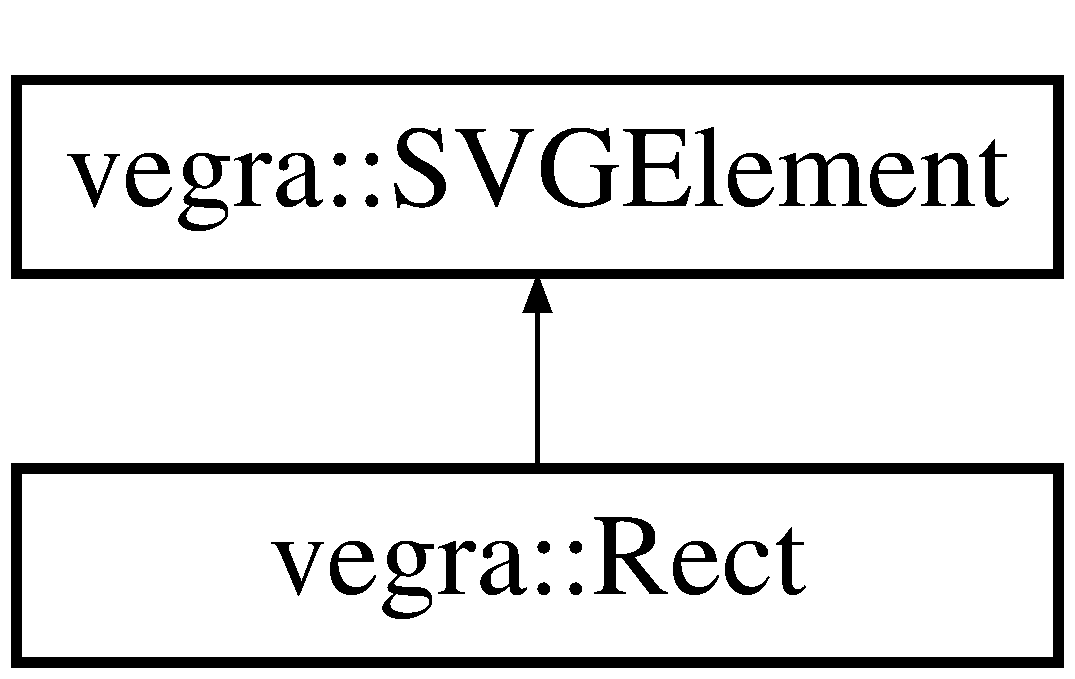
\includegraphics[height=2.000000cm]{structvegra_1_1Rect}
\end{center}
\end{figure}
\subsection*{Public Member Functions}
\begin{DoxyCompactItemize}
\item 
\mbox{\hyperlink{structvegra_1_1Rect_a5f7d578540b861188333858882d8fc09}{Rect}} ()
\item 
void \mbox{\hyperlink{structvegra_1_1Rect_a58f3d61bd592c6344d319da7eb7cee5c}{add}} ()
\item 
void \mbox{\hyperlink{structvegra_1_1Rect_a3d6fd5f777b1faca1a850e9ba5328434}{add}} (\mbox{\hyperlink{structvegra_1_1SVGElement}{vegra\+::\+S\+V\+G\+Element}} $\ast$element)
\item 
{\footnotesize template$<$typename... Args$>$ }\\void \mbox{\hyperlink{structvegra_1_1Rect_ae1d87cebca7a5eb3c9a2ce5e4782c2a6}{add}} (\mbox{\hyperlink{structvegra_1_1SVGElement}{vegra\+::\+S\+V\+G\+Element}} $\ast$element, Args... args)
\item 
std\+::string \mbox{\hyperlink{structvegra_1_1Rect_a2f18ab8fb102c330de2e388a4f5cb324}{compose\+Element}} ()
\item 
void \mbox{\hyperlink{structvegra_1_1Rect_a1a0b6b2fa5804f2554f62d41c3a156f3}{wrap\+Element}} ()
\item 
void \mbox{\hyperlink{structvegra_1_1Rect_ae4f9a214f68dd59bc5fc5fda2c746add}{set\+Pos}} (\mbox{\hyperlink{structvegra_1_1Position}{vegra\+::\+Position}} pos)
\item 
void \mbox{\hyperlink{structvegra_1_1Rect_a5aae282d87d00e7912620eee07b1c588}{set\+Size}} (\mbox{\hyperlink{structvegra_1_1Size}{vegra\+::\+Size}} size)
\item 
void \mbox{\hyperlink{structvegra_1_1Rect_a646ee5d4a13f051a08e03efcaecf8afb}{set\+Stroke}} (\mbox{\hyperlink{structvegra_1_1Stroke}{vegra\+::\+Stroke}} stroke)
\item 
void \mbox{\hyperlink{structvegra_1_1Rect_a42038bb978010d425ac7418bb5ca8c43}{set\+Fill}} (\mbox{\hyperlink{structvegra_1_1Fill}{vegra\+::\+Fill}} fill)
\item 
\mbox{\hyperlink{namespacevegra_a2722f5eceb74f65746a02a57b71d125e}{S\+V\+G\+Element\+List}} \mbox{\hyperlink{structvegra_1_1Rect_a8d02abb21b9198be69cd888a20ff664a}{get\+Elements}} ()
\begin{DoxyCompactList}\small\item\em Funtion to get svg element list. \end{DoxyCompactList}\item 
\mbox{\hyperlink{structvegra_1_1Position}{vegra\+::\+Position}} \mbox{\hyperlink{structvegra_1_1Rect_a78df3821c00d24877cd16e5d356e2d3a}{get\+Pos}} ()
\item 
\mbox{\hyperlink{structvegra_1_1Size}{vegra\+::\+Size}} \mbox{\hyperlink{structvegra_1_1Rect_a509bc44c11ff4c5da09b9f0a8f989f3e}{get\+Size}} ()
\item 
\mbox{\hyperlink{structvegra_1_1Stroke}{vegra\+::\+Stroke}} \mbox{\hyperlink{structvegra_1_1Rect_aa6015029c78e89030e2e125e53be7e31}{get\+Stroke}} ()
\item 
\mbox{\hyperlink{structvegra_1_1Fill}{vegra\+::\+Fill}} \mbox{\hyperlink{structvegra_1_1Rect_a3abeedcf01ddec54812aa4c0f21c1877}{get\+Fill}} ()
\item 
std\+::string \mbox{\hyperlink{structvegra_1_1Rect_a914ba572d7bda0dcb40b6f112d959f04}{get\+Element}} () override
\end{DoxyCompactItemize}


\subsection{Constructor \& Destructor Documentation}
\mbox{\Hypertarget{structvegra_1_1Rect_a5f7d578540b861188333858882d8fc09}\label{structvegra_1_1Rect_a5f7d578540b861188333858882d8fc09}} 
\index{vegra\+::\+Rect@{vegra\+::\+Rect}!Rect@{Rect}}
\index{Rect@{Rect}!vegra\+::\+Rect@{vegra\+::\+Rect}}
\subsubsection{\texorpdfstring{Rect()}{Rect()}}
{\footnotesize\ttfamily vegra\+::\+Rect\+::\+Rect (\begin{DoxyParamCaption}{ }\end{DoxyParamCaption})\hspace{0.3cm}{\ttfamily [inline]}}



\subsection{Member Function Documentation}
\mbox{\Hypertarget{structvegra_1_1Rect_a58f3d61bd592c6344d319da7eb7cee5c}\label{structvegra_1_1Rect_a58f3d61bd592c6344d319da7eb7cee5c}} 
\index{vegra\+::\+Rect@{vegra\+::\+Rect}!add@{add}}
\index{add@{add}!vegra\+::\+Rect@{vegra\+::\+Rect}}
\subsubsection{\texorpdfstring{add()}{add()}\hspace{0.1cm}{\footnotesize\ttfamily [1/3]}}
{\footnotesize\ttfamily void vegra\+::\+Rect\+::add (\begin{DoxyParamCaption}{ }\end{DoxyParamCaption})\hspace{0.3cm}{\ttfamily [inline]}}

\mbox{\Hypertarget{structvegra_1_1Rect_a3d6fd5f777b1faca1a850e9ba5328434}\label{structvegra_1_1Rect_a3d6fd5f777b1faca1a850e9ba5328434}} 
\index{vegra\+::\+Rect@{vegra\+::\+Rect}!add@{add}}
\index{add@{add}!vegra\+::\+Rect@{vegra\+::\+Rect}}
\subsubsection{\texorpdfstring{add()}{add()}\hspace{0.1cm}{\footnotesize\ttfamily [2/3]}}
{\footnotesize\ttfamily void vegra\+::\+Rect\+::add (\begin{DoxyParamCaption}\item[{\mbox{\hyperlink{structvegra_1_1SVGElement}{vegra\+::\+S\+V\+G\+Element}} $\ast$}]{element }\end{DoxyParamCaption})\hspace{0.3cm}{\ttfamily [inline]}}

\mbox{\Hypertarget{structvegra_1_1Rect_ae1d87cebca7a5eb3c9a2ce5e4782c2a6}\label{structvegra_1_1Rect_ae1d87cebca7a5eb3c9a2ce5e4782c2a6}} 
\index{vegra\+::\+Rect@{vegra\+::\+Rect}!add@{add}}
\index{add@{add}!vegra\+::\+Rect@{vegra\+::\+Rect}}
\subsubsection{\texorpdfstring{add()}{add()}\hspace{0.1cm}{\footnotesize\ttfamily [3/3]}}
{\footnotesize\ttfamily template$<$typename... Args$>$ \\
void vegra\+::\+Rect\+::add (\begin{DoxyParamCaption}\item[{\mbox{\hyperlink{structvegra_1_1SVGElement}{vegra\+::\+S\+V\+G\+Element}} $\ast$}]{element,  }\item[{Args...}]{args }\end{DoxyParamCaption})\hspace{0.3cm}{\ttfamily [inline]}}

\mbox{\Hypertarget{structvegra_1_1Rect_a2f18ab8fb102c330de2e388a4f5cb324}\label{structvegra_1_1Rect_a2f18ab8fb102c330de2e388a4f5cb324}} 
\index{vegra\+::\+Rect@{vegra\+::\+Rect}!compose\+Element@{compose\+Element}}
\index{compose\+Element@{compose\+Element}!vegra\+::\+Rect@{vegra\+::\+Rect}}
\subsubsection{\texorpdfstring{compose\+Element()}{composeElement()}}
{\footnotesize\ttfamily std\+::string vegra\+::\+Rect\+::compose\+Element (\begin{DoxyParamCaption}{ }\end{DoxyParamCaption})\hspace{0.3cm}{\ttfamily [inline]}}

\mbox{\Hypertarget{structvegra_1_1Rect_a914ba572d7bda0dcb40b6f112d959f04}\label{structvegra_1_1Rect_a914ba572d7bda0dcb40b6f112d959f04}} 
\index{vegra\+::\+Rect@{vegra\+::\+Rect}!get\+Element@{get\+Element}}
\index{get\+Element@{get\+Element}!vegra\+::\+Rect@{vegra\+::\+Rect}}
\subsubsection{\texorpdfstring{get\+Element()}{getElement()}}
{\footnotesize\ttfamily std\+::string vegra\+::\+Rect\+::get\+Element (\begin{DoxyParamCaption}{ }\end{DoxyParamCaption})\hspace{0.3cm}{\ttfamily [inline]}, {\ttfamily [override]}, {\ttfamily [virtual]}}



Implements \mbox{\hyperlink{structvegra_1_1SVGElement_a17fa30b9de97e1541eaa1f6888145de2}{vegra\+::\+S\+V\+G\+Element}}.

\mbox{\Hypertarget{structvegra_1_1Rect_a8d02abb21b9198be69cd888a20ff664a}\label{structvegra_1_1Rect_a8d02abb21b9198be69cd888a20ff664a}} 
\index{vegra\+::\+Rect@{vegra\+::\+Rect}!get\+Elements@{get\+Elements}}
\index{get\+Elements@{get\+Elements}!vegra\+::\+Rect@{vegra\+::\+Rect}}
\subsubsection{\texorpdfstring{get\+Elements()}{getElements()}}
{\footnotesize\ttfamily \mbox{\hyperlink{namespacevegra_a2722f5eceb74f65746a02a57b71d125e}{S\+V\+G\+Element\+List}} vegra\+::\+Rect\+::get\+Elements (\begin{DoxyParamCaption}{ }\end{DoxyParamCaption})\hspace{0.3cm}{\ttfamily [inline]}}



Funtion to get svg element list. 

\mbox{\Hypertarget{structvegra_1_1Rect_a3abeedcf01ddec54812aa4c0f21c1877}\label{structvegra_1_1Rect_a3abeedcf01ddec54812aa4c0f21c1877}} 
\index{vegra\+::\+Rect@{vegra\+::\+Rect}!get\+Fill@{get\+Fill}}
\index{get\+Fill@{get\+Fill}!vegra\+::\+Rect@{vegra\+::\+Rect}}
\subsubsection{\texorpdfstring{get\+Fill()}{getFill()}}
{\footnotesize\ttfamily \mbox{\hyperlink{structvegra_1_1Fill}{vegra\+::\+Fill}} vegra\+::\+Rect\+::get\+Fill (\begin{DoxyParamCaption}{ }\end{DoxyParamCaption})\hspace{0.3cm}{\ttfamily [inline]}}

\mbox{\Hypertarget{structvegra_1_1Rect_a78df3821c00d24877cd16e5d356e2d3a}\label{structvegra_1_1Rect_a78df3821c00d24877cd16e5d356e2d3a}} 
\index{vegra\+::\+Rect@{vegra\+::\+Rect}!get\+Pos@{get\+Pos}}
\index{get\+Pos@{get\+Pos}!vegra\+::\+Rect@{vegra\+::\+Rect}}
\subsubsection{\texorpdfstring{get\+Pos()}{getPos()}}
{\footnotesize\ttfamily \mbox{\hyperlink{structvegra_1_1Position}{vegra\+::\+Position}} vegra\+::\+Rect\+::get\+Pos (\begin{DoxyParamCaption}{ }\end{DoxyParamCaption})\hspace{0.3cm}{\ttfamily [inline]}}

\mbox{\Hypertarget{structvegra_1_1Rect_a509bc44c11ff4c5da09b9f0a8f989f3e}\label{structvegra_1_1Rect_a509bc44c11ff4c5da09b9f0a8f989f3e}} 
\index{vegra\+::\+Rect@{vegra\+::\+Rect}!get\+Size@{get\+Size}}
\index{get\+Size@{get\+Size}!vegra\+::\+Rect@{vegra\+::\+Rect}}
\subsubsection{\texorpdfstring{get\+Size()}{getSize()}}
{\footnotesize\ttfamily \mbox{\hyperlink{structvegra_1_1Size}{vegra\+::\+Size}} vegra\+::\+Rect\+::get\+Size (\begin{DoxyParamCaption}{ }\end{DoxyParamCaption})\hspace{0.3cm}{\ttfamily [inline]}}

\mbox{\Hypertarget{structvegra_1_1Rect_aa6015029c78e89030e2e125e53be7e31}\label{structvegra_1_1Rect_aa6015029c78e89030e2e125e53be7e31}} 
\index{vegra\+::\+Rect@{vegra\+::\+Rect}!get\+Stroke@{get\+Stroke}}
\index{get\+Stroke@{get\+Stroke}!vegra\+::\+Rect@{vegra\+::\+Rect}}
\subsubsection{\texorpdfstring{get\+Stroke()}{getStroke()}}
{\footnotesize\ttfamily \mbox{\hyperlink{structvegra_1_1Stroke}{vegra\+::\+Stroke}} vegra\+::\+Rect\+::get\+Stroke (\begin{DoxyParamCaption}{ }\end{DoxyParamCaption})\hspace{0.3cm}{\ttfamily [inline]}}

\mbox{\Hypertarget{structvegra_1_1Rect_a42038bb978010d425ac7418bb5ca8c43}\label{structvegra_1_1Rect_a42038bb978010d425ac7418bb5ca8c43}} 
\index{vegra\+::\+Rect@{vegra\+::\+Rect}!set\+Fill@{set\+Fill}}
\index{set\+Fill@{set\+Fill}!vegra\+::\+Rect@{vegra\+::\+Rect}}
\subsubsection{\texorpdfstring{set\+Fill()}{setFill()}}
{\footnotesize\ttfamily void vegra\+::\+Rect\+::set\+Fill (\begin{DoxyParamCaption}\item[{\mbox{\hyperlink{structvegra_1_1Fill}{vegra\+::\+Fill}}}]{fill }\end{DoxyParamCaption})\hspace{0.3cm}{\ttfamily [inline]}}

\mbox{\Hypertarget{structvegra_1_1Rect_ae4f9a214f68dd59bc5fc5fda2c746add}\label{structvegra_1_1Rect_ae4f9a214f68dd59bc5fc5fda2c746add}} 
\index{vegra\+::\+Rect@{vegra\+::\+Rect}!set\+Pos@{set\+Pos}}
\index{set\+Pos@{set\+Pos}!vegra\+::\+Rect@{vegra\+::\+Rect}}
\subsubsection{\texorpdfstring{set\+Pos()}{setPos()}}
{\footnotesize\ttfamily void vegra\+::\+Rect\+::set\+Pos (\begin{DoxyParamCaption}\item[{\mbox{\hyperlink{structvegra_1_1Position}{vegra\+::\+Position}}}]{pos }\end{DoxyParamCaption})\hspace{0.3cm}{\ttfamily [inline]}}

\mbox{\Hypertarget{structvegra_1_1Rect_a5aae282d87d00e7912620eee07b1c588}\label{structvegra_1_1Rect_a5aae282d87d00e7912620eee07b1c588}} 
\index{vegra\+::\+Rect@{vegra\+::\+Rect}!set\+Size@{set\+Size}}
\index{set\+Size@{set\+Size}!vegra\+::\+Rect@{vegra\+::\+Rect}}
\subsubsection{\texorpdfstring{set\+Size()}{setSize()}}
{\footnotesize\ttfamily void vegra\+::\+Rect\+::set\+Size (\begin{DoxyParamCaption}\item[{\mbox{\hyperlink{structvegra_1_1Size}{vegra\+::\+Size}}}]{size }\end{DoxyParamCaption})\hspace{0.3cm}{\ttfamily [inline]}}

\mbox{\Hypertarget{structvegra_1_1Rect_a646ee5d4a13f051a08e03efcaecf8afb}\label{structvegra_1_1Rect_a646ee5d4a13f051a08e03efcaecf8afb}} 
\index{vegra\+::\+Rect@{vegra\+::\+Rect}!set\+Stroke@{set\+Stroke}}
\index{set\+Stroke@{set\+Stroke}!vegra\+::\+Rect@{vegra\+::\+Rect}}
\subsubsection{\texorpdfstring{set\+Stroke()}{setStroke()}}
{\footnotesize\ttfamily void vegra\+::\+Rect\+::set\+Stroke (\begin{DoxyParamCaption}\item[{\mbox{\hyperlink{structvegra_1_1Stroke}{vegra\+::\+Stroke}}}]{stroke }\end{DoxyParamCaption})\hspace{0.3cm}{\ttfamily [inline]}}

\mbox{\Hypertarget{structvegra_1_1Rect_a1a0b6b2fa5804f2554f62d41c3a156f3}\label{structvegra_1_1Rect_a1a0b6b2fa5804f2554f62d41c3a156f3}} 
\index{vegra\+::\+Rect@{vegra\+::\+Rect}!wrap\+Element@{wrap\+Element}}
\index{wrap\+Element@{wrap\+Element}!vegra\+::\+Rect@{vegra\+::\+Rect}}
\subsubsection{\texorpdfstring{wrap\+Element()}{wrapElement()}}
{\footnotesize\ttfamily void vegra\+::\+Rect\+::wrap\+Element (\begin{DoxyParamCaption}{ }\end{DoxyParamCaption})\hspace{0.3cm}{\ttfamily [inline]}, {\ttfamily [virtual]}}



Implements \mbox{\hyperlink{structvegra_1_1SVGElement_a1369400ebe57287f1b5beb5f0234d8d7}{vegra\+::\+S\+V\+G\+Element}}.



The documentation for this struct was generated from the following file\+:\begin{DoxyCompactItemize}
\item 
/home/raghu/\+Development/vegra/include/\mbox{\hyperlink{rect_8h}{rect.\+h}}\end{DoxyCompactItemize}

\hypertarget{structvegra_1_1Size}{}\section{vegra\+:\+:Size Struct Reference}
\label{structvegra_1_1Size}\index{vegra\+::\+Size@{vegra\+::\+Size}}


{\ttfamily \#include $<$attrib.\+h$>$}

\subsection*{Public Member Functions}
\begin{DoxyCompactItemize}
\item 
\mbox{\hyperlink{structvegra_1_1Size_a6d5058f3d438e24fca92f3c261ecd7a8}{Size}} ()
\item 
\mbox{\hyperlink{structvegra_1_1Size_af92638bf9795f8c562cc7424f212e985}{Size}} (int \mbox{\hyperlink{structvegra_1_1Size_ab88c99e72a1579a2ac00f10133c5f23d}{height}}, int \mbox{\hyperlink{structvegra_1_1Size_ae71295e2c36b57cb0a71e4c4974ec753}{width}})
\item 
void \mbox{\hyperlink{structvegra_1_1Size_a7788fabbf4bc7ad2b23f5b4b113983a8}{set\+Size}} (int \mbox{\hyperlink{structvegra_1_1Size_ab88c99e72a1579a2ac00f10133c5f23d}{height}}, int \mbox{\hyperlink{structvegra_1_1Size_ae71295e2c36b57cb0a71e4c4974ec753}{width}})
\item 
void \mbox{\hyperlink{structvegra_1_1Size_a92f779e3bcaae71cc2f80d3a87506a30}{set\+Height}} (int \mbox{\hyperlink{structvegra_1_1Size_ab88c99e72a1579a2ac00f10133c5f23d}{height}})
\item 
void \mbox{\hyperlink{structvegra_1_1Size_a916716ce017fced6ec41612142289798}{set\+Width}} (int \mbox{\hyperlink{structvegra_1_1Size_ae71295e2c36b57cb0a71e4c4974ec753}{width}})
\item 
\mbox{\hyperlink{structvegra_1_1Size}{Size}} \mbox{\hyperlink{structvegra_1_1Size_afe0b7cbe050d2419ca8bc59880be8799}{get\+Size}} ()
\item 
int \mbox{\hyperlink{structvegra_1_1Size_a58e78996257b9b625babb0c217767759}{get\+Height}} ()
\item 
int \mbox{\hyperlink{structvegra_1_1Size_af565490734a7ef2975c1e359e44c4a9e}{get\+Width}} ()
\end{DoxyCompactItemize}
\subsection*{Public Attributes}
\begin{DoxyCompactItemize}
\item 
int \mbox{\hyperlink{structvegra_1_1Size_ab88c99e72a1579a2ac00f10133c5f23d}{height}}
\item 
int \mbox{\hyperlink{structvegra_1_1Size_ae71295e2c36b57cb0a71e4c4974ec753}{width}}
\end{DoxyCompactItemize}


\subsection{Constructor \& Destructor Documentation}
\mbox{\Hypertarget{structvegra_1_1Size_a6d5058f3d438e24fca92f3c261ecd7a8}\label{structvegra_1_1Size_a6d5058f3d438e24fca92f3c261ecd7a8}} 
\index{vegra\+::\+Size@{vegra\+::\+Size}!Size@{Size}}
\index{Size@{Size}!vegra\+::\+Size@{vegra\+::\+Size}}
\subsubsection{\texorpdfstring{Size()}{Size()}\hspace{0.1cm}{\footnotesize\ttfamily [1/2]}}
{\footnotesize\ttfamily vegra\+::\+Size\+::\+Size (\begin{DoxyParamCaption}{ }\end{DoxyParamCaption})\hspace{0.3cm}{\ttfamily [inline]}}

\mbox{\Hypertarget{structvegra_1_1Size_af92638bf9795f8c562cc7424f212e985}\label{structvegra_1_1Size_af92638bf9795f8c562cc7424f212e985}} 
\index{vegra\+::\+Size@{vegra\+::\+Size}!Size@{Size}}
\index{Size@{Size}!vegra\+::\+Size@{vegra\+::\+Size}}
\subsubsection{\texorpdfstring{Size()}{Size()}\hspace{0.1cm}{\footnotesize\ttfamily [2/2]}}
{\footnotesize\ttfamily vegra\+::\+Size\+::\+Size (\begin{DoxyParamCaption}\item[{int}]{height,  }\item[{int}]{width }\end{DoxyParamCaption})\hspace{0.3cm}{\ttfamily [inline]}}



\subsection{Member Function Documentation}
\mbox{\Hypertarget{structvegra_1_1Size_a58e78996257b9b625babb0c217767759}\label{structvegra_1_1Size_a58e78996257b9b625babb0c217767759}} 
\index{vegra\+::\+Size@{vegra\+::\+Size}!get\+Height@{get\+Height}}
\index{get\+Height@{get\+Height}!vegra\+::\+Size@{vegra\+::\+Size}}
\subsubsection{\texorpdfstring{get\+Height()}{getHeight()}}
{\footnotesize\ttfamily int vegra\+::\+Size\+::get\+Height (\begin{DoxyParamCaption}{ }\end{DoxyParamCaption})\hspace{0.3cm}{\ttfamily [inline]}}

\mbox{\Hypertarget{structvegra_1_1Size_afe0b7cbe050d2419ca8bc59880be8799}\label{structvegra_1_1Size_afe0b7cbe050d2419ca8bc59880be8799}} 
\index{vegra\+::\+Size@{vegra\+::\+Size}!get\+Size@{get\+Size}}
\index{get\+Size@{get\+Size}!vegra\+::\+Size@{vegra\+::\+Size}}
\subsubsection{\texorpdfstring{get\+Size()}{getSize()}}
{\footnotesize\ttfamily \mbox{\hyperlink{structvegra_1_1Size}{Size}} vegra\+::\+Size\+::get\+Size (\begin{DoxyParamCaption}{ }\end{DoxyParamCaption})\hspace{0.3cm}{\ttfamily [inline]}}

\mbox{\Hypertarget{structvegra_1_1Size_af565490734a7ef2975c1e359e44c4a9e}\label{structvegra_1_1Size_af565490734a7ef2975c1e359e44c4a9e}} 
\index{vegra\+::\+Size@{vegra\+::\+Size}!get\+Width@{get\+Width}}
\index{get\+Width@{get\+Width}!vegra\+::\+Size@{vegra\+::\+Size}}
\subsubsection{\texorpdfstring{get\+Width()}{getWidth()}}
{\footnotesize\ttfamily int vegra\+::\+Size\+::get\+Width (\begin{DoxyParamCaption}{ }\end{DoxyParamCaption})\hspace{0.3cm}{\ttfamily [inline]}}

\mbox{\Hypertarget{structvegra_1_1Size_a92f779e3bcaae71cc2f80d3a87506a30}\label{structvegra_1_1Size_a92f779e3bcaae71cc2f80d3a87506a30}} 
\index{vegra\+::\+Size@{vegra\+::\+Size}!set\+Height@{set\+Height}}
\index{set\+Height@{set\+Height}!vegra\+::\+Size@{vegra\+::\+Size}}
\subsubsection{\texorpdfstring{set\+Height()}{setHeight()}}
{\footnotesize\ttfamily void vegra\+::\+Size\+::set\+Height (\begin{DoxyParamCaption}\item[{int}]{height }\end{DoxyParamCaption})\hspace{0.3cm}{\ttfamily [inline]}}

\mbox{\Hypertarget{structvegra_1_1Size_a7788fabbf4bc7ad2b23f5b4b113983a8}\label{structvegra_1_1Size_a7788fabbf4bc7ad2b23f5b4b113983a8}} 
\index{vegra\+::\+Size@{vegra\+::\+Size}!set\+Size@{set\+Size}}
\index{set\+Size@{set\+Size}!vegra\+::\+Size@{vegra\+::\+Size}}
\subsubsection{\texorpdfstring{set\+Size()}{setSize()}}
{\footnotesize\ttfamily void vegra\+::\+Size\+::set\+Size (\begin{DoxyParamCaption}\item[{int}]{height,  }\item[{int}]{width }\end{DoxyParamCaption})\hspace{0.3cm}{\ttfamily [inline]}}

\mbox{\Hypertarget{structvegra_1_1Size_a916716ce017fced6ec41612142289798}\label{structvegra_1_1Size_a916716ce017fced6ec41612142289798}} 
\index{vegra\+::\+Size@{vegra\+::\+Size}!set\+Width@{set\+Width}}
\index{set\+Width@{set\+Width}!vegra\+::\+Size@{vegra\+::\+Size}}
\subsubsection{\texorpdfstring{set\+Width()}{setWidth()}}
{\footnotesize\ttfamily void vegra\+::\+Size\+::set\+Width (\begin{DoxyParamCaption}\item[{int}]{width }\end{DoxyParamCaption})\hspace{0.3cm}{\ttfamily [inline]}}



\subsection{Member Data Documentation}
\mbox{\Hypertarget{structvegra_1_1Size_ab88c99e72a1579a2ac00f10133c5f23d}\label{structvegra_1_1Size_ab88c99e72a1579a2ac00f10133c5f23d}} 
\index{vegra\+::\+Size@{vegra\+::\+Size}!height@{height}}
\index{height@{height}!vegra\+::\+Size@{vegra\+::\+Size}}
\subsubsection{\texorpdfstring{height}{height}}
{\footnotesize\ttfamily int vegra\+::\+Size\+::height}

\mbox{\Hypertarget{structvegra_1_1Size_ae71295e2c36b57cb0a71e4c4974ec753}\label{structvegra_1_1Size_ae71295e2c36b57cb0a71e4c4974ec753}} 
\index{vegra\+::\+Size@{vegra\+::\+Size}!width@{width}}
\index{width@{width}!vegra\+::\+Size@{vegra\+::\+Size}}
\subsubsection{\texorpdfstring{width}{width}}
{\footnotesize\ttfamily int vegra\+::\+Size\+::width}



The documentation for this struct was generated from the following file\+:\begin{DoxyCompactItemize}
\item 
/home/raghu/\+Development/vegra/include/\mbox{\hyperlink{attrib_8h}{attrib.\+h}}\end{DoxyCompactItemize}

\hypertarget{structvegra_1_1Stroke}{}\section{vegra\+:\+:Stroke Struct Reference}
\label{structvegra_1_1Stroke}\index{vegra\+::\+Stroke@{vegra\+::\+Stroke}}


Attribute to outline the element.  




{\ttfamily \#include $<$attrib.\+h$>$}

\subsection*{Public Types}
\begin{DoxyCompactItemize}
\item 
using \mbox{\hyperlink{structvegra_1_1Stroke_af5a2b4ee71962d044ebb7a309b22bb8a}{i\+\_\+pair}} = std\+::pair$<$ int, int $>$
\end{DoxyCompactItemize}
\subsection*{Public Member Functions}
\begin{DoxyCompactItemize}
\item 
\mbox{\hyperlink{structvegra_1_1Stroke_a64be83054d51672b104626cefdb303d4}{Stroke}} ()
\item 
\mbox{\hyperlink{structvegra_1_1Stroke_a48ed9ac6ddee81297219d76534a71f8e}{Stroke}} (std\+::string \mbox{\hyperlink{structvegra_1_1Stroke_a407c59871f2ade9be29d2c5dfe28d21d}{color}}, size\+\_\+t \mbox{\hyperlink{structvegra_1_1Stroke_a95579e85bd704a94840674bbdee34304}{width}}, \mbox{\hyperlink{structvegra_1_1Stroke_af5a2b4ee71962d044ebb7a309b22bb8a}{i\+\_\+pair}} \mbox{\hyperlink{structvegra_1_1Stroke_a649828302bf54741b69ffeca87cbabbf}{dasharray}}, size\+\_\+t \mbox{\hyperlink{structvegra_1_1Stroke_aac202e47f5066fcd16cd4e1b1296214d}{dashoffset}}, std\+::string \mbox{\hyperlink{structvegra_1_1Stroke_a67a29aa2a553bf490f8556dd526fcfcf}{linecap}}, double \mbox{\hyperlink{structvegra_1_1Stroke_a1549534821eb8e96632f405af3c59d26}{opacity}})
\item 
void \mbox{\hyperlink{structvegra_1_1Stroke_a8404fd7b631e78bfb3021f026abbcc10}{set\+Color}} (std\+::string \mbox{\hyperlink{structvegra_1_1Stroke_a407c59871f2ade9be29d2c5dfe28d21d}{color}})
\item 
void \mbox{\hyperlink{structvegra_1_1Stroke_ae9aedb99ff7526cb922192b8faacd2bf}{set\+Width}} (size\+\_\+t \mbox{\hyperlink{structvegra_1_1Stroke_a95579e85bd704a94840674bbdee34304}{width}})
\item 
void \mbox{\hyperlink{structvegra_1_1Stroke_a440e67289da779bb73144d7b4a73a6f3}{set\+Dash\+Array}} (\mbox{\hyperlink{structvegra_1_1Stroke_af5a2b4ee71962d044ebb7a309b22bb8a}{i\+\_\+pair}} \mbox{\hyperlink{structvegra_1_1Stroke_a649828302bf54741b69ffeca87cbabbf}{dasharray}})
\item 
void \mbox{\hyperlink{structvegra_1_1Stroke_ae4581f2780ef60bdebc0af0d575c8c63}{set\+Dash\+Offset}} (size\+\_\+t \mbox{\hyperlink{structvegra_1_1Stroke_aac202e47f5066fcd16cd4e1b1296214d}{dashoffset}})
\item 
void \mbox{\hyperlink{structvegra_1_1Stroke_ac7e1d55eba440b657c5ec4d193fd8a0f}{set\+Linecap}} (std\+::string \mbox{\hyperlink{structvegra_1_1Stroke_a67a29aa2a553bf490f8556dd526fcfcf}{linecap}})
\item 
void \mbox{\hyperlink{structvegra_1_1Stroke_a5eae4ca7fa12a23911f7b959760f88fa}{set\+Opacity}} (double \mbox{\hyperlink{structvegra_1_1Stroke_a1549534821eb8e96632f405af3c59d26}{opacity}})
\item 
std\+::string \mbox{\hyperlink{structvegra_1_1Stroke_a6fa9107861ae4898e29baac94866f229}{get\+Color}} ()
\item 
size\+\_\+t \mbox{\hyperlink{structvegra_1_1Stroke_a695152e114e79817e53bb3d67e137228}{get\+Width}} ()
\item 
\mbox{\hyperlink{structvegra_1_1Stroke_af5a2b4ee71962d044ebb7a309b22bb8a}{i\+\_\+pair}} \mbox{\hyperlink{structvegra_1_1Stroke_ae396487e8776add16ddd78cdd436034f}{get\+Dash\+Aray}} ()
\item 
size\+\_\+t \mbox{\hyperlink{structvegra_1_1Stroke_aae4b7e22569da832b7279dd1e98c6dea}{get\+Dash\+Offset}} ()
\item 
std\+::string \mbox{\hyperlink{structvegra_1_1Stroke_a5a9f290ed03bc2dbcd120ffc7d0bd52d}{get\+Linecap}} ()
\item 
double \mbox{\hyperlink{structvegra_1_1Stroke_ab472a9732c83c1e4547d32ccf4b91877}{get\+Opacity}} ()
\end{DoxyCompactItemize}
\subsection*{Public Attributes}
\begin{DoxyCompactItemize}
\item 
std\+::string \mbox{\hyperlink{structvegra_1_1Stroke_a407c59871f2ade9be29d2c5dfe28d21d}{color}}
\item 
size\+\_\+t \mbox{\hyperlink{structvegra_1_1Stroke_a95579e85bd704a94840674bbdee34304}{width}}
\begin{DoxyCompactList}\small\item\em stroke \end{DoxyCompactList}\item 
\mbox{\hyperlink{structvegra_1_1Stroke_af5a2b4ee71962d044ebb7a309b22bb8a}{i\+\_\+pair}} \mbox{\hyperlink{structvegra_1_1Stroke_a649828302bf54741b69ffeca87cbabbf}{dasharray}}
\begin{DoxyCompactList}\small\item\em stroke-\/width \end{DoxyCompactList}\item 
size\+\_\+t \mbox{\hyperlink{structvegra_1_1Stroke_aac202e47f5066fcd16cd4e1b1296214d}{dashoffset}}
\begin{DoxyCompactList}\small\item\em stroke-\/dasharray \end{DoxyCompactList}\item 
std\+::string \mbox{\hyperlink{structvegra_1_1Stroke_a67a29aa2a553bf490f8556dd526fcfcf}{linecap}}
\begin{DoxyCompactList}\small\item\em stroke-\/dashoffset \end{DoxyCompactList}\item 
double \mbox{\hyperlink{structvegra_1_1Stroke_a1549534821eb8e96632f405af3c59d26}{opacity}}
\begin{DoxyCompactList}\small\item\em stroke-\/linecap \end{DoxyCompactList}\end{DoxyCompactItemize}


\subsection{Detailed Description}
Attribute to outline the element. 

\subsection{Member Typedef Documentation}
\mbox{\Hypertarget{structvegra_1_1Stroke_af5a2b4ee71962d044ebb7a309b22bb8a}\label{structvegra_1_1Stroke_af5a2b4ee71962d044ebb7a309b22bb8a}} 
\index{vegra\+::\+Stroke@{vegra\+::\+Stroke}!i\+\_\+pair@{i\+\_\+pair}}
\index{i\+\_\+pair@{i\+\_\+pair}!vegra\+::\+Stroke@{vegra\+::\+Stroke}}
\subsubsection{\texorpdfstring{i\+\_\+pair}{i\_pair}}
{\footnotesize\ttfamily using \mbox{\hyperlink{structvegra_1_1Stroke_af5a2b4ee71962d044ebb7a309b22bb8a}{vegra\+::\+Stroke\+::i\+\_\+pair}} =  std\+::pair$<$int, int$>$}



\subsection{Constructor \& Destructor Documentation}
\mbox{\Hypertarget{structvegra_1_1Stroke_a64be83054d51672b104626cefdb303d4}\label{structvegra_1_1Stroke_a64be83054d51672b104626cefdb303d4}} 
\index{vegra\+::\+Stroke@{vegra\+::\+Stroke}!Stroke@{Stroke}}
\index{Stroke@{Stroke}!vegra\+::\+Stroke@{vegra\+::\+Stroke}}
\subsubsection{\texorpdfstring{Stroke()}{Stroke()}\hspace{0.1cm}{\footnotesize\ttfamily [1/2]}}
{\footnotesize\ttfamily vegra\+::\+Stroke\+::\+Stroke (\begin{DoxyParamCaption}{ }\end{DoxyParamCaption})\hspace{0.3cm}{\ttfamily [inline]}}

\mbox{\Hypertarget{structvegra_1_1Stroke_a48ed9ac6ddee81297219d76534a71f8e}\label{structvegra_1_1Stroke_a48ed9ac6ddee81297219d76534a71f8e}} 
\index{vegra\+::\+Stroke@{vegra\+::\+Stroke}!Stroke@{Stroke}}
\index{Stroke@{Stroke}!vegra\+::\+Stroke@{vegra\+::\+Stroke}}
\subsubsection{\texorpdfstring{Stroke()}{Stroke()}\hspace{0.1cm}{\footnotesize\ttfamily [2/2]}}
{\footnotesize\ttfamily vegra\+::\+Stroke\+::\+Stroke (\begin{DoxyParamCaption}\item[{std\+::string}]{color,  }\item[{size\+\_\+t}]{width,  }\item[{\mbox{\hyperlink{structvegra_1_1Stroke_af5a2b4ee71962d044ebb7a309b22bb8a}{i\+\_\+pair}}}]{dasharray,  }\item[{size\+\_\+t}]{dashoffset,  }\item[{std\+::string}]{linecap,  }\item[{double}]{opacity }\end{DoxyParamCaption})\hspace{0.3cm}{\ttfamily [inline]}}



\subsection{Member Function Documentation}
\mbox{\Hypertarget{structvegra_1_1Stroke_a6fa9107861ae4898e29baac94866f229}\label{structvegra_1_1Stroke_a6fa9107861ae4898e29baac94866f229}} 
\index{vegra\+::\+Stroke@{vegra\+::\+Stroke}!get\+Color@{get\+Color}}
\index{get\+Color@{get\+Color}!vegra\+::\+Stroke@{vegra\+::\+Stroke}}
\subsubsection{\texorpdfstring{get\+Color()}{getColor()}}
{\footnotesize\ttfamily std\+::string vegra\+::\+Stroke\+::get\+Color (\begin{DoxyParamCaption}{ }\end{DoxyParamCaption})\hspace{0.3cm}{\ttfamily [inline]}}

\mbox{\Hypertarget{structvegra_1_1Stroke_ae396487e8776add16ddd78cdd436034f}\label{structvegra_1_1Stroke_ae396487e8776add16ddd78cdd436034f}} 
\index{vegra\+::\+Stroke@{vegra\+::\+Stroke}!get\+Dash\+Aray@{get\+Dash\+Aray}}
\index{get\+Dash\+Aray@{get\+Dash\+Aray}!vegra\+::\+Stroke@{vegra\+::\+Stroke}}
\subsubsection{\texorpdfstring{get\+Dash\+Aray()}{getDashAray()}}
{\footnotesize\ttfamily \mbox{\hyperlink{structvegra_1_1Stroke_af5a2b4ee71962d044ebb7a309b22bb8a}{i\+\_\+pair}} vegra\+::\+Stroke\+::get\+Dash\+Aray (\begin{DoxyParamCaption}{ }\end{DoxyParamCaption})\hspace{0.3cm}{\ttfamily [inline]}}

\mbox{\Hypertarget{structvegra_1_1Stroke_aae4b7e22569da832b7279dd1e98c6dea}\label{structvegra_1_1Stroke_aae4b7e22569da832b7279dd1e98c6dea}} 
\index{vegra\+::\+Stroke@{vegra\+::\+Stroke}!get\+Dash\+Offset@{get\+Dash\+Offset}}
\index{get\+Dash\+Offset@{get\+Dash\+Offset}!vegra\+::\+Stroke@{vegra\+::\+Stroke}}
\subsubsection{\texorpdfstring{get\+Dash\+Offset()}{getDashOffset()}}
{\footnotesize\ttfamily size\+\_\+t vegra\+::\+Stroke\+::get\+Dash\+Offset (\begin{DoxyParamCaption}{ }\end{DoxyParamCaption})\hspace{0.3cm}{\ttfamily [inline]}}

\mbox{\Hypertarget{structvegra_1_1Stroke_a5a9f290ed03bc2dbcd120ffc7d0bd52d}\label{structvegra_1_1Stroke_a5a9f290ed03bc2dbcd120ffc7d0bd52d}} 
\index{vegra\+::\+Stroke@{vegra\+::\+Stroke}!get\+Linecap@{get\+Linecap}}
\index{get\+Linecap@{get\+Linecap}!vegra\+::\+Stroke@{vegra\+::\+Stroke}}
\subsubsection{\texorpdfstring{get\+Linecap()}{getLinecap()}}
{\footnotesize\ttfamily std\+::string vegra\+::\+Stroke\+::get\+Linecap (\begin{DoxyParamCaption}{ }\end{DoxyParamCaption})\hspace{0.3cm}{\ttfamily [inline]}}

\mbox{\Hypertarget{structvegra_1_1Stroke_ab472a9732c83c1e4547d32ccf4b91877}\label{structvegra_1_1Stroke_ab472a9732c83c1e4547d32ccf4b91877}} 
\index{vegra\+::\+Stroke@{vegra\+::\+Stroke}!get\+Opacity@{get\+Opacity}}
\index{get\+Opacity@{get\+Opacity}!vegra\+::\+Stroke@{vegra\+::\+Stroke}}
\subsubsection{\texorpdfstring{get\+Opacity()}{getOpacity()}}
{\footnotesize\ttfamily double vegra\+::\+Stroke\+::get\+Opacity (\begin{DoxyParamCaption}{ }\end{DoxyParamCaption})\hspace{0.3cm}{\ttfamily [inline]}}

\mbox{\Hypertarget{structvegra_1_1Stroke_a695152e114e79817e53bb3d67e137228}\label{structvegra_1_1Stroke_a695152e114e79817e53bb3d67e137228}} 
\index{vegra\+::\+Stroke@{vegra\+::\+Stroke}!get\+Width@{get\+Width}}
\index{get\+Width@{get\+Width}!vegra\+::\+Stroke@{vegra\+::\+Stroke}}
\subsubsection{\texorpdfstring{get\+Width()}{getWidth()}}
{\footnotesize\ttfamily size\+\_\+t vegra\+::\+Stroke\+::get\+Width (\begin{DoxyParamCaption}{ }\end{DoxyParamCaption})\hspace{0.3cm}{\ttfamily [inline]}}

\mbox{\Hypertarget{structvegra_1_1Stroke_a8404fd7b631e78bfb3021f026abbcc10}\label{structvegra_1_1Stroke_a8404fd7b631e78bfb3021f026abbcc10}} 
\index{vegra\+::\+Stroke@{vegra\+::\+Stroke}!set\+Color@{set\+Color}}
\index{set\+Color@{set\+Color}!vegra\+::\+Stroke@{vegra\+::\+Stroke}}
\subsubsection{\texorpdfstring{set\+Color()}{setColor()}}
{\footnotesize\ttfamily void vegra\+::\+Stroke\+::set\+Color (\begin{DoxyParamCaption}\item[{std\+::string}]{color }\end{DoxyParamCaption})\hspace{0.3cm}{\ttfamily [inline]}}

\mbox{\Hypertarget{structvegra_1_1Stroke_a440e67289da779bb73144d7b4a73a6f3}\label{structvegra_1_1Stroke_a440e67289da779bb73144d7b4a73a6f3}} 
\index{vegra\+::\+Stroke@{vegra\+::\+Stroke}!set\+Dash\+Array@{set\+Dash\+Array}}
\index{set\+Dash\+Array@{set\+Dash\+Array}!vegra\+::\+Stroke@{vegra\+::\+Stroke}}
\subsubsection{\texorpdfstring{set\+Dash\+Array()}{setDashArray()}}
{\footnotesize\ttfamily void vegra\+::\+Stroke\+::set\+Dash\+Array (\begin{DoxyParamCaption}\item[{\mbox{\hyperlink{structvegra_1_1Stroke_af5a2b4ee71962d044ebb7a309b22bb8a}{i\+\_\+pair}}}]{dasharray }\end{DoxyParamCaption})\hspace{0.3cm}{\ttfamily [inline]}}

\mbox{\Hypertarget{structvegra_1_1Stroke_ae4581f2780ef60bdebc0af0d575c8c63}\label{structvegra_1_1Stroke_ae4581f2780ef60bdebc0af0d575c8c63}} 
\index{vegra\+::\+Stroke@{vegra\+::\+Stroke}!set\+Dash\+Offset@{set\+Dash\+Offset}}
\index{set\+Dash\+Offset@{set\+Dash\+Offset}!vegra\+::\+Stroke@{vegra\+::\+Stroke}}
\subsubsection{\texorpdfstring{set\+Dash\+Offset()}{setDashOffset()}}
{\footnotesize\ttfamily void vegra\+::\+Stroke\+::set\+Dash\+Offset (\begin{DoxyParamCaption}\item[{size\+\_\+t}]{dashoffset }\end{DoxyParamCaption})\hspace{0.3cm}{\ttfamily [inline]}}

\mbox{\Hypertarget{structvegra_1_1Stroke_ac7e1d55eba440b657c5ec4d193fd8a0f}\label{structvegra_1_1Stroke_ac7e1d55eba440b657c5ec4d193fd8a0f}} 
\index{vegra\+::\+Stroke@{vegra\+::\+Stroke}!set\+Linecap@{set\+Linecap}}
\index{set\+Linecap@{set\+Linecap}!vegra\+::\+Stroke@{vegra\+::\+Stroke}}
\subsubsection{\texorpdfstring{set\+Linecap()}{setLinecap()}}
{\footnotesize\ttfamily void vegra\+::\+Stroke\+::set\+Linecap (\begin{DoxyParamCaption}\item[{std\+::string}]{linecap }\end{DoxyParamCaption})\hspace{0.3cm}{\ttfamily [inline]}}

\mbox{\Hypertarget{structvegra_1_1Stroke_a5eae4ca7fa12a23911f7b959760f88fa}\label{structvegra_1_1Stroke_a5eae4ca7fa12a23911f7b959760f88fa}} 
\index{vegra\+::\+Stroke@{vegra\+::\+Stroke}!set\+Opacity@{set\+Opacity}}
\index{set\+Opacity@{set\+Opacity}!vegra\+::\+Stroke@{vegra\+::\+Stroke}}
\subsubsection{\texorpdfstring{set\+Opacity()}{setOpacity()}}
{\footnotesize\ttfamily void vegra\+::\+Stroke\+::set\+Opacity (\begin{DoxyParamCaption}\item[{double}]{opacity }\end{DoxyParamCaption})\hspace{0.3cm}{\ttfamily [inline]}}

\mbox{\Hypertarget{structvegra_1_1Stroke_ae9aedb99ff7526cb922192b8faacd2bf}\label{structvegra_1_1Stroke_ae9aedb99ff7526cb922192b8faacd2bf}} 
\index{vegra\+::\+Stroke@{vegra\+::\+Stroke}!set\+Width@{set\+Width}}
\index{set\+Width@{set\+Width}!vegra\+::\+Stroke@{vegra\+::\+Stroke}}
\subsubsection{\texorpdfstring{set\+Width()}{setWidth()}}
{\footnotesize\ttfamily void vegra\+::\+Stroke\+::set\+Width (\begin{DoxyParamCaption}\item[{size\+\_\+t}]{width }\end{DoxyParamCaption})\hspace{0.3cm}{\ttfamily [inline]}}



\subsection{Member Data Documentation}
\mbox{\Hypertarget{structvegra_1_1Stroke_a407c59871f2ade9be29d2c5dfe28d21d}\label{structvegra_1_1Stroke_a407c59871f2ade9be29d2c5dfe28d21d}} 
\index{vegra\+::\+Stroke@{vegra\+::\+Stroke}!color@{color}}
\index{color@{color}!vegra\+::\+Stroke@{vegra\+::\+Stroke}}
\subsubsection{\texorpdfstring{color}{color}}
{\footnotesize\ttfamily std\+::string vegra\+::\+Stroke\+::color}

\mbox{\Hypertarget{structvegra_1_1Stroke_a649828302bf54741b69ffeca87cbabbf}\label{structvegra_1_1Stroke_a649828302bf54741b69ffeca87cbabbf}} 
\index{vegra\+::\+Stroke@{vegra\+::\+Stroke}!dasharray@{dasharray}}
\index{dasharray@{dasharray}!vegra\+::\+Stroke@{vegra\+::\+Stroke}}
\subsubsection{\texorpdfstring{dasharray}{dasharray}}
{\footnotesize\ttfamily \mbox{\hyperlink{structvegra_1_1Stroke_af5a2b4ee71962d044ebb7a309b22bb8a}{i\+\_\+pair}} vegra\+::\+Stroke\+::dasharray}



stroke-\/width 

\mbox{\Hypertarget{structvegra_1_1Stroke_aac202e47f5066fcd16cd4e1b1296214d}\label{structvegra_1_1Stroke_aac202e47f5066fcd16cd4e1b1296214d}} 
\index{vegra\+::\+Stroke@{vegra\+::\+Stroke}!dashoffset@{dashoffset}}
\index{dashoffset@{dashoffset}!vegra\+::\+Stroke@{vegra\+::\+Stroke}}
\subsubsection{\texorpdfstring{dashoffset}{dashoffset}}
{\footnotesize\ttfamily size\+\_\+t vegra\+::\+Stroke\+::dashoffset}



stroke-\/dasharray 

\mbox{\Hypertarget{structvegra_1_1Stroke_a67a29aa2a553bf490f8556dd526fcfcf}\label{structvegra_1_1Stroke_a67a29aa2a553bf490f8556dd526fcfcf}} 
\index{vegra\+::\+Stroke@{vegra\+::\+Stroke}!linecap@{linecap}}
\index{linecap@{linecap}!vegra\+::\+Stroke@{vegra\+::\+Stroke}}
\subsubsection{\texorpdfstring{linecap}{linecap}}
{\footnotesize\ttfamily std\+::string vegra\+::\+Stroke\+::linecap}



stroke-\/dashoffset 

\mbox{\Hypertarget{structvegra_1_1Stroke_a1549534821eb8e96632f405af3c59d26}\label{structvegra_1_1Stroke_a1549534821eb8e96632f405af3c59d26}} 
\index{vegra\+::\+Stroke@{vegra\+::\+Stroke}!opacity@{opacity}}
\index{opacity@{opacity}!vegra\+::\+Stroke@{vegra\+::\+Stroke}}
\subsubsection{\texorpdfstring{opacity}{opacity}}
{\footnotesize\ttfamily double vegra\+::\+Stroke\+::opacity}



stroke-\/linecap 

\mbox{\Hypertarget{structvegra_1_1Stroke_a95579e85bd704a94840674bbdee34304}\label{structvegra_1_1Stroke_a95579e85bd704a94840674bbdee34304}} 
\index{vegra\+::\+Stroke@{vegra\+::\+Stroke}!width@{width}}
\index{width@{width}!vegra\+::\+Stroke@{vegra\+::\+Stroke}}
\subsubsection{\texorpdfstring{width}{width}}
{\footnotesize\ttfamily size\+\_\+t vegra\+::\+Stroke\+::width}



stroke 



The documentation for this struct was generated from the following file\+:\begin{DoxyCompactItemize}
\item 
/home/raghu/\+Development/vegra/include/\mbox{\hyperlink{attrib_8h}{attrib.\+h}}\end{DoxyCompactItemize}

\hypertarget{structvegra_1_1SVG}{}\section{vegra\+:\+:S\+VG Struct Reference}
\label{structvegra_1_1SVG}\index{vegra\+::\+S\+VG@{vegra\+::\+S\+VG}}


\mbox{\hyperlink{structvegra_1_1SVG}{S\+VG}} element.  




{\ttfamily \#include $<$vegra.\+h$>$}

Inheritance diagram for vegra\+:\+:S\+VG\+:\begin{figure}[H]
\begin{center}
\leavevmode
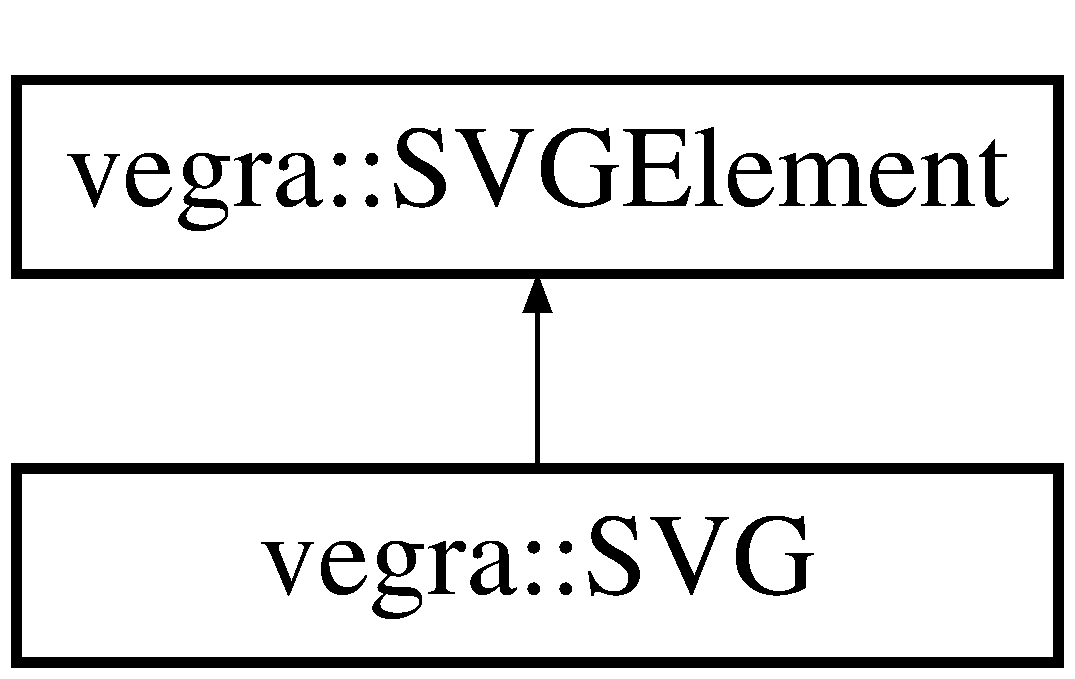
\includegraphics[height=2.000000cm]{structvegra_1_1SVG}
\end{center}
\end{figure}
\subsection*{Public Member Functions}
\begin{DoxyCompactItemize}
\item 
\mbox{\hyperlink{structvegra_1_1SVG_a3fd44691284da36fbf659b230e870950}{S\+VG}} ()
\item 
void \mbox{\hyperlink{structvegra_1_1SVG_a018d3d664341f68deff0a170885bac05}{add}} ()
\item 
void \mbox{\hyperlink{structvegra_1_1SVG_a7d1da466cecd8260ae1e9514b15a2ec0}{add}} (\mbox{\hyperlink{structvegra_1_1SVGElement}{vegra\+::\+S\+V\+G\+Element}} $\ast$element)
\item 
{\footnotesize template$<$typename... Args$>$ }\\void \mbox{\hyperlink{structvegra_1_1SVG_a4c942cc22cecde5d82d796773aab772b}{add}} (\mbox{\hyperlink{structvegra_1_1SVGElement}{vegra\+::\+S\+V\+G\+Element}} $\ast$element, Args... args)
\item 
std\+::string \mbox{\hyperlink{structvegra_1_1SVG_aa24a923e5c6195e143623e141ada168b}{compose\+Element}} ()
\item 
void \mbox{\hyperlink{structvegra_1_1SVG_ae7192d00544cf372f5dfed2b2436c973}{wrap\+Element}} ()
\item 
bool \mbox{\hyperlink{structvegra_1_1SVG_a185b8b4ad59002b8fc921a288f69f9d9}{check\+If\+S\+V\+G\+Exists}} ()
\item 
void \mbox{\hyperlink{structvegra_1_1SVG_a739917fb674392c8a92ce56c609daf9c}{save\+S\+VG}} ()
\item 
void \mbox{\hyperlink{structvegra_1_1SVG_a02f78ba059b1ce0e659ee368fb6a782a}{create\+New\+Title}} ()
\item 
void \mbox{\hyperlink{structvegra_1_1SVG_a90d8788e7776685d3da401ce8a9a8596}{close}} ()
\begin{DoxyCompactList}\small\item\em save svg and close the svg \end{DoxyCompactList}\item 
\mbox{\hyperlink{namespacevegra_a2722f5eceb74f65746a02a57b71d125e}{S\+V\+G\+Element\+List}} \mbox{\hyperlink{structvegra_1_1SVG_a6096892ee39e3680fddd6657a98b7a75}{get\+Elements}} ()
\begin{DoxyCompactList}\small\item\em Funtion to get svg element list. \end{DoxyCompactList}\item 
\mbox{\hyperlink{structvegra_1_1Position}{vegra\+::\+Position}} \mbox{\hyperlink{structvegra_1_1SVG_a6d7a82c399cdf3ea7e078b66a8bbf024}{get\+Pos}} ()
\begin{DoxyCompactList}\small\item\em Function to get \mbox{\hyperlink{structvegra_1_1Position}{Position}} of \mbox{\hyperlink{structvegra_1_1SVG}{S\+VG}} in the D\+OM. \end{DoxyCompactList}\item 
\mbox{\hyperlink{structvegra_1_1Size}{vegra\+::\+Size}} \mbox{\hyperlink{structvegra_1_1SVG_ad1b80e84f2eeccbbf7c039812f6c35fa}{get\+Size}} ()
\begin{DoxyCompactList}\small\item\em Function to get \mbox{\hyperlink{structvegra_1_1Size}{Size}} of \mbox{\hyperlink{structvegra_1_1SVG}{S\+VG}} in the D\+OM. \end{DoxyCompactList}\item 
std\+::string \mbox{\hyperlink{structvegra_1_1SVG_aec9681b5ca49e9cdd48297677b18151b}{get\+Element}} () override
\item 
void \mbox{\hyperlink{structvegra_1_1SVG_a6468964d098acbdd91da3cac55e6f6b8}{set\+Pos}} (\mbox{\hyperlink{structvegra_1_1Position}{vegra\+::\+Position}} pos)
\begin{DoxyCompactList}\small\item\em Function to set \mbox{\hyperlink{structvegra_1_1Position}{Position}} of \mbox{\hyperlink{structvegra_1_1SVG}{S\+VG}} in the D\+OM. \end{DoxyCompactList}\item 
void \mbox{\hyperlink{structvegra_1_1SVG_ad80b2990559293806eeb8223bb7a8dc4}{set\+Size}} (\mbox{\hyperlink{structvegra_1_1Size}{vegra\+::\+Size}} size)
\begin{DoxyCompactList}\small\item\em Function to set \mbox{\hyperlink{structvegra_1_1Size}{Size}} of \mbox{\hyperlink{structvegra_1_1SVG}{S\+VG}} wrt D\+OM. \end{DoxyCompactList}\end{DoxyCompactItemize}


\subsection{Detailed Description}
\mbox{\hyperlink{structvegra_1_1SVG}{S\+VG}} element. 

\subsection{Constructor \& Destructor Documentation}
\mbox{\Hypertarget{structvegra_1_1SVG_a3fd44691284da36fbf659b230e870950}\label{structvegra_1_1SVG_a3fd44691284da36fbf659b230e870950}} 
\index{vegra\+::\+S\+VG@{vegra\+::\+S\+VG}!S\+VG@{S\+VG}}
\index{S\+VG@{S\+VG}!vegra\+::\+S\+VG@{vegra\+::\+S\+VG}}
\subsubsection{\texorpdfstring{S\+V\+G()}{SVG()}}
{\footnotesize\ttfamily vegra\+::\+S\+V\+G\+::\+S\+VG (\begin{DoxyParamCaption}{ }\end{DoxyParamCaption})\hspace{0.3cm}{\ttfamily [inline]}}



\subsection{Member Function Documentation}
\mbox{\Hypertarget{structvegra_1_1SVG_a018d3d664341f68deff0a170885bac05}\label{structvegra_1_1SVG_a018d3d664341f68deff0a170885bac05}} 
\index{vegra\+::\+S\+VG@{vegra\+::\+S\+VG}!add@{add}}
\index{add@{add}!vegra\+::\+S\+VG@{vegra\+::\+S\+VG}}
\subsubsection{\texorpdfstring{add()}{add()}\hspace{0.1cm}{\footnotesize\ttfamily [1/3]}}
{\footnotesize\ttfamily void vegra\+::\+S\+V\+G\+::add (\begin{DoxyParamCaption}{ }\end{DoxyParamCaption})\hspace{0.3cm}{\ttfamily [inline]}}

\mbox{\Hypertarget{structvegra_1_1SVG_a7d1da466cecd8260ae1e9514b15a2ec0}\label{structvegra_1_1SVG_a7d1da466cecd8260ae1e9514b15a2ec0}} 
\index{vegra\+::\+S\+VG@{vegra\+::\+S\+VG}!add@{add}}
\index{add@{add}!vegra\+::\+S\+VG@{vegra\+::\+S\+VG}}
\subsubsection{\texorpdfstring{add()}{add()}\hspace{0.1cm}{\footnotesize\ttfamily [2/3]}}
{\footnotesize\ttfamily void vegra\+::\+S\+V\+G\+::add (\begin{DoxyParamCaption}\item[{\mbox{\hyperlink{structvegra_1_1SVGElement}{vegra\+::\+S\+V\+G\+Element}} $\ast$}]{element }\end{DoxyParamCaption})\hspace{0.3cm}{\ttfamily [inline]}}

\mbox{\Hypertarget{structvegra_1_1SVG_a4c942cc22cecde5d82d796773aab772b}\label{structvegra_1_1SVG_a4c942cc22cecde5d82d796773aab772b}} 
\index{vegra\+::\+S\+VG@{vegra\+::\+S\+VG}!add@{add}}
\index{add@{add}!vegra\+::\+S\+VG@{vegra\+::\+S\+VG}}
\subsubsection{\texorpdfstring{add()}{add()}\hspace{0.1cm}{\footnotesize\ttfamily [3/3]}}
{\footnotesize\ttfamily template$<$typename... Args$>$ \\
void vegra\+::\+S\+V\+G\+::add (\begin{DoxyParamCaption}\item[{\mbox{\hyperlink{structvegra_1_1SVGElement}{vegra\+::\+S\+V\+G\+Element}} $\ast$}]{element,  }\item[{Args...}]{args }\end{DoxyParamCaption})\hspace{0.3cm}{\ttfamily [inline]}}

\mbox{\Hypertarget{structvegra_1_1SVG_a185b8b4ad59002b8fc921a288f69f9d9}\label{structvegra_1_1SVG_a185b8b4ad59002b8fc921a288f69f9d9}} 
\index{vegra\+::\+S\+VG@{vegra\+::\+S\+VG}!check\+If\+S\+V\+G\+Exists@{check\+If\+S\+V\+G\+Exists}}
\index{check\+If\+S\+V\+G\+Exists@{check\+If\+S\+V\+G\+Exists}!vegra\+::\+S\+VG@{vegra\+::\+S\+VG}}
\subsubsection{\texorpdfstring{check\+If\+S\+V\+G\+Exists()}{checkIfSVGExists()}}
{\footnotesize\ttfamily bool vegra\+::\+S\+V\+G\+::check\+If\+S\+V\+G\+Exists (\begin{DoxyParamCaption}{ }\end{DoxyParamCaption})\hspace{0.3cm}{\ttfamily [inline]}}

\mbox{\Hypertarget{structvegra_1_1SVG_a90d8788e7776685d3da401ce8a9a8596}\label{structvegra_1_1SVG_a90d8788e7776685d3da401ce8a9a8596}} 
\index{vegra\+::\+S\+VG@{vegra\+::\+S\+VG}!close@{close}}
\index{close@{close}!vegra\+::\+S\+VG@{vegra\+::\+S\+VG}}
\subsubsection{\texorpdfstring{close()}{close()}}
{\footnotesize\ttfamily void vegra\+::\+S\+V\+G\+::close (\begin{DoxyParamCaption}{ }\end{DoxyParamCaption})\hspace{0.3cm}{\ttfamily [inline]}}



save svg and close the svg 

\mbox{\Hypertarget{structvegra_1_1SVG_aa24a923e5c6195e143623e141ada168b}\label{structvegra_1_1SVG_aa24a923e5c6195e143623e141ada168b}} 
\index{vegra\+::\+S\+VG@{vegra\+::\+S\+VG}!compose\+Element@{compose\+Element}}
\index{compose\+Element@{compose\+Element}!vegra\+::\+S\+VG@{vegra\+::\+S\+VG}}
\subsubsection{\texorpdfstring{compose\+Element()}{composeElement()}}
{\footnotesize\ttfamily std\+::string vegra\+::\+S\+V\+G\+::compose\+Element (\begin{DoxyParamCaption}{ }\end{DoxyParamCaption})\hspace{0.3cm}{\ttfamily [inline]}}

\mbox{\Hypertarget{structvegra_1_1SVG_a02f78ba059b1ce0e659ee368fb6a782a}\label{structvegra_1_1SVG_a02f78ba059b1ce0e659ee368fb6a782a}} 
\index{vegra\+::\+S\+VG@{vegra\+::\+S\+VG}!create\+New\+Title@{create\+New\+Title}}
\index{create\+New\+Title@{create\+New\+Title}!vegra\+::\+S\+VG@{vegra\+::\+S\+VG}}
\subsubsection{\texorpdfstring{create\+New\+Title()}{createNewTitle()}}
{\footnotesize\ttfamily void vegra\+::\+S\+V\+G\+::create\+New\+Title (\begin{DoxyParamCaption}{ }\end{DoxyParamCaption})\hspace{0.3cm}{\ttfamily [inline]}}

\mbox{\Hypertarget{structvegra_1_1SVG_aec9681b5ca49e9cdd48297677b18151b}\label{structvegra_1_1SVG_aec9681b5ca49e9cdd48297677b18151b}} 
\index{vegra\+::\+S\+VG@{vegra\+::\+S\+VG}!get\+Element@{get\+Element}}
\index{get\+Element@{get\+Element}!vegra\+::\+S\+VG@{vegra\+::\+S\+VG}}
\subsubsection{\texorpdfstring{get\+Element()}{getElement()}}
{\footnotesize\ttfamily std\+::string vegra\+::\+S\+V\+G\+::get\+Element (\begin{DoxyParamCaption}{ }\end{DoxyParamCaption})\hspace{0.3cm}{\ttfamily [inline]}, {\ttfamily [override]}, {\ttfamily [virtual]}}



Implements \mbox{\hyperlink{structvegra_1_1SVGElement_a17fa30b9de97e1541eaa1f6888145de2}{vegra\+::\+S\+V\+G\+Element}}.

\mbox{\Hypertarget{structvegra_1_1SVG_a6096892ee39e3680fddd6657a98b7a75}\label{structvegra_1_1SVG_a6096892ee39e3680fddd6657a98b7a75}} 
\index{vegra\+::\+S\+VG@{vegra\+::\+S\+VG}!get\+Elements@{get\+Elements}}
\index{get\+Elements@{get\+Elements}!vegra\+::\+S\+VG@{vegra\+::\+S\+VG}}
\subsubsection{\texorpdfstring{get\+Elements()}{getElements()}}
{\footnotesize\ttfamily \mbox{\hyperlink{namespacevegra_a2722f5eceb74f65746a02a57b71d125e}{S\+V\+G\+Element\+List}} vegra\+::\+S\+V\+G\+::get\+Elements (\begin{DoxyParamCaption}{ }\end{DoxyParamCaption})\hspace{0.3cm}{\ttfamily [inline]}}



Funtion to get svg element list. 

\mbox{\Hypertarget{structvegra_1_1SVG_a6d7a82c399cdf3ea7e078b66a8bbf024}\label{structvegra_1_1SVG_a6d7a82c399cdf3ea7e078b66a8bbf024}} 
\index{vegra\+::\+S\+VG@{vegra\+::\+S\+VG}!get\+Pos@{get\+Pos}}
\index{get\+Pos@{get\+Pos}!vegra\+::\+S\+VG@{vegra\+::\+S\+VG}}
\subsubsection{\texorpdfstring{get\+Pos()}{getPos()}}
{\footnotesize\ttfamily \mbox{\hyperlink{structvegra_1_1Position}{vegra\+::\+Position}} vegra\+::\+S\+V\+G\+::get\+Pos (\begin{DoxyParamCaption}{ }\end{DoxyParamCaption})\hspace{0.3cm}{\ttfamily [inline]}}



Function to get \mbox{\hyperlink{structvegra_1_1Position}{Position}} of \mbox{\hyperlink{structvegra_1_1SVG}{S\+VG}} in the D\+OM. 

\mbox{\Hypertarget{structvegra_1_1SVG_ad1b80e84f2eeccbbf7c039812f6c35fa}\label{structvegra_1_1SVG_ad1b80e84f2eeccbbf7c039812f6c35fa}} 
\index{vegra\+::\+S\+VG@{vegra\+::\+S\+VG}!get\+Size@{get\+Size}}
\index{get\+Size@{get\+Size}!vegra\+::\+S\+VG@{vegra\+::\+S\+VG}}
\subsubsection{\texorpdfstring{get\+Size()}{getSize()}}
{\footnotesize\ttfamily \mbox{\hyperlink{structvegra_1_1Size}{vegra\+::\+Size}} vegra\+::\+S\+V\+G\+::get\+Size (\begin{DoxyParamCaption}{ }\end{DoxyParamCaption})\hspace{0.3cm}{\ttfamily [inline]}}



Function to get \mbox{\hyperlink{structvegra_1_1Size}{Size}} of \mbox{\hyperlink{structvegra_1_1SVG}{S\+VG}} in the D\+OM. 

\mbox{\Hypertarget{structvegra_1_1SVG_a739917fb674392c8a92ce56c609daf9c}\label{structvegra_1_1SVG_a739917fb674392c8a92ce56c609daf9c}} 
\index{vegra\+::\+S\+VG@{vegra\+::\+S\+VG}!save\+S\+VG@{save\+S\+VG}}
\index{save\+S\+VG@{save\+S\+VG}!vegra\+::\+S\+VG@{vegra\+::\+S\+VG}}
\subsubsection{\texorpdfstring{save\+S\+V\+G()}{saveSVG()}}
{\footnotesize\ttfamily void vegra\+::\+S\+V\+G\+::save\+S\+VG (\begin{DoxyParamCaption}{ }\end{DoxyParamCaption})\hspace{0.3cm}{\ttfamily [inline]}}

\mbox{\Hypertarget{structvegra_1_1SVG_a6468964d098acbdd91da3cac55e6f6b8}\label{structvegra_1_1SVG_a6468964d098acbdd91da3cac55e6f6b8}} 
\index{vegra\+::\+S\+VG@{vegra\+::\+S\+VG}!set\+Pos@{set\+Pos}}
\index{set\+Pos@{set\+Pos}!vegra\+::\+S\+VG@{vegra\+::\+S\+VG}}
\subsubsection{\texorpdfstring{set\+Pos()}{setPos()}}
{\footnotesize\ttfamily void vegra\+::\+S\+V\+G\+::set\+Pos (\begin{DoxyParamCaption}\item[{\mbox{\hyperlink{structvegra_1_1Position}{vegra\+::\+Position}}}]{pos }\end{DoxyParamCaption})\hspace{0.3cm}{\ttfamily [inline]}}



Function to set \mbox{\hyperlink{structvegra_1_1Position}{Position}} of \mbox{\hyperlink{structvegra_1_1SVG}{S\+VG}} in the D\+OM. 

\mbox{\Hypertarget{structvegra_1_1SVG_ad80b2990559293806eeb8223bb7a8dc4}\label{structvegra_1_1SVG_ad80b2990559293806eeb8223bb7a8dc4}} 
\index{vegra\+::\+S\+VG@{vegra\+::\+S\+VG}!set\+Size@{set\+Size}}
\index{set\+Size@{set\+Size}!vegra\+::\+S\+VG@{vegra\+::\+S\+VG}}
\subsubsection{\texorpdfstring{set\+Size()}{setSize()}}
{\footnotesize\ttfamily void vegra\+::\+S\+V\+G\+::set\+Size (\begin{DoxyParamCaption}\item[{\mbox{\hyperlink{structvegra_1_1Size}{vegra\+::\+Size}}}]{size }\end{DoxyParamCaption})\hspace{0.3cm}{\ttfamily [inline]}}



Function to set \mbox{\hyperlink{structvegra_1_1Size}{Size}} of \mbox{\hyperlink{structvegra_1_1SVG}{S\+VG}} wrt D\+OM. 

\mbox{\Hypertarget{structvegra_1_1SVG_ae7192d00544cf372f5dfed2b2436c973}\label{structvegra_1_1SVG_ae7192d00544cf372f5dfed2b2436c973}} 
\index{vegra\+::\+S\+VG@{vegra\+::\+S\+VG}!wrap\+Element@{wrap\+Element}}
\index{wrap\+Element@{wrap\+Element}!vegra\+::\+S\+VG@{vegra\+::\+S\+VG}}
\subsubsection{\texorpdfstring{wrap\+Element()}{wrapElement()}}
{\footnotesize\ttfamily void vegra\+::\+S\+V\+G\+::wrap\+Element (\begin{DoxyParamCaption}{ }\end{DoxyParamCaption})\hspace{0.3cm}{\ttfamily [inline]}, {\ttfamily [virtual]}}



Implements \mbox{\hyperlink{structvegra_1_1SVGElement_a1369400ebe57287f1b5beb5f0234d8d7}{vegra\+::\+S\+V\+G\+Element}}.



The documentation for this struct was generated from the following file\+:\begin{DoxyCompactItemize}
\item 
/home/raghu/\+Development/vegra/include/\mbox{\hyperlink{vegra_8h}{vegra.\+h}}\end{DoxyCompactItemize}

\hypertarget{structvegra_1_1SVGElement}{}\section{vegra\+:\+:S\+V\+G\+Element Struct Reference}
\label{structvegra_1_1SVGElement}\index{vegra\+::\+S\+V\+G\+Element@{vegra\+::\+S\+V\+G\+Element}}


\mbox{\hyperlink{structvegra_1_1SVGElement}{S\+V\+G\+Element}} -\/ Parent class for all svg elements.  




{\ttfamily \#include $<$elements.\+h$>$}

Inheritance diagram for vegra\+:\+:S\+V\+G\+Element\+:\begin{figure}[H]
\begin{center}
\leavevmode
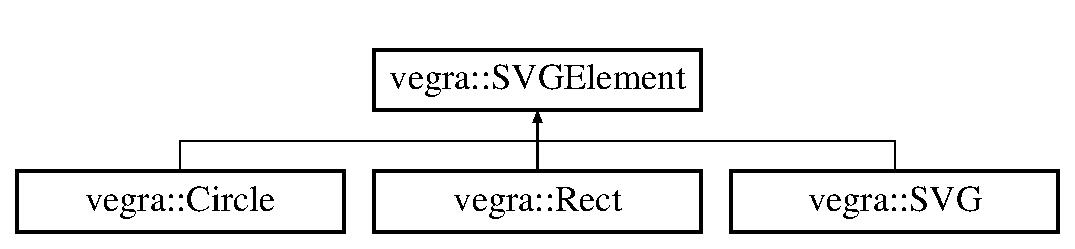
\includegraphics[height=2.000000cm]{structvegra_1_1SVGElement}
\end{center}
\end{figure}
\subsection*{Public Member Functions}
\begin{DoxyCompactItemize}
\item 
\mbox{\hyperlink{structvegra_1_1SVGElement_a08b7a1eb40780c9aec388ebd3f715e19}{S\+V\+G\+Element}} ()
\item 
virtual void \mbox{\hyperlink{structvegra_1_1SVGElement_a1369400ebe57287f1b5beb5f0234d8d7}{wrap\+Element}} ()=0
\item 
virtual std\+::string \mbox{\hyperlink{structvegra_1_1SVGElement_a17fa30b9de97e1541eaa1f6888145de2}{get\+Element}} ()=0
\end{DoxyCompactItemize}


\subsection{Detailed Description}
\mbox{\hyperlink{structvegra_1_1SVGElement}{S\+V\+G\+Element}} -\/ Parent class for all svg elements. 

\subsection{Constructor \& Destructor Documentation}
\mbox{\Hypertarget{structvegra_1_1SVGElement_a08b7a1eb40780c9aec388ebd3f715e19}\label{structvegra_1_1SVGElement_a08b7a1eb40780c9aec388ebd3f715e19}} 
\index{vegra\+::\+S\+V\+G\+Element@{vegra\+::\+S\+V\+G\+Element}!S\+V\+G\+Element@{S\+V\+G\+Element}}
\index{S\+V\+G\+Element@{S\+V\+G\+Element}!vegra\+::\+S\+V\+G\+Element@{vegra\+::\+S\+V\+G\+Element}}
\subsubsection{\texorpdfstring{S\+V\+G\+Element()}{SVGElement()}}
{\footnotesize\ttfamily vegra\+::\+S\+V\+G\+Element\+::\+S\+V\+G\+Element (\begin{DoxyParamCaption}{ }\end{DoxyParamCaption})\hspace{0.3cm}{\ttfamily [inline]}}



\subsection{Member Function Documentation}
\mbox{\Hypertarget{structvegra_1_1SVGElement_a17fa30b9de97e1541eaa1f6888145de2}\label{structvegra_1_1SVGElement_a17fa30b9de97e1541eaa1f6888145de2}} 
\index{vegra\+::\+S\+V\+G\+Element@{vegra\+::\+S\+V\+G\+Element}!get\+Element@{get\+Element}}
\index{get\+Element@{get\+Element}!vegra\+::\+S\+V\+G\+Element@{vegra\+::\+S\+V\+G\+Element}}
\subsubsection{\texorpdfstring{get\+Element()}{getElement()}}
{\footnotesize\ttfamily virtual std\+::string vegra\+::\+S\+V\+G\+Element\+::get\+Element (\begin{DoxyParamCaption}{ }\end{DoxyParamCaption})\hspace{0.3cm}{\ttfamily [pure virtual]}}



Implemented in \mbox{\hyperlink{structvegra_1_1SVG_aec9681b5ca49e9cdd48297677b18151b}{vegra\+::\+S\+VG}}, \mbox{\hyperlink{structvegra_1_1Rect_a914ba572d7bda0dcb40b6f112d959f04}{vegra\+::\+Rect}}, and \mbox{\hyperlink{structvegra_1_1Circle_a50bdbe7e4b29530b131e7a1157190b00}{vegra\+::\+Circle}}.

\mbox{\Hypertarget{structvegra_1_1SVGElement_a1369400ebe57287f1b5beb5f0234d8d7}\label{structvegra_1_1SVGElement_a1369400ebe57287f1b5beb5f0234d8d7}} 
\index{vegra\+::\+S\+V\+G\+Element@{vegra\+::\+S\+V\+G\+Element}!wrap\+Element@{wrap\+Element}}
\index{wrap\+Element@{wrap\+Element}!vegra\+::\+S\+V\+G\+Element@{vegra\+::\+S\+V\+G\+Element}}
\subsubsection{\texorpdfstring{wrap\+Element()}{wrapElement()}}
{\footnotesize\ttfamily virtual void vegra\+::\+S\+V\+G\+Element\+::wrap\+Element (\begin{DoxyParamCaption}{ }\end{DoxyParamCaption})\hspace{0.3cm}{\ttfamily [pure virtual]}}



Implemented in \mbox{\hyperlink{structvegra_1_1SVG_ae7192d00544cf372f5dfed2b2436c973}{vegra\+::\+S\+VG}}, \mbox{\hyperlink{structvegra_1_1Circle_a67bfa48e7697a6ee3e7c79fed1129a3c}{vegra\+::\+Circle}}, and \mbox{\hyperlink{structvegra_1_1Rect_a1a0b6b2fa5804f2554f62d41c3a156f3}{vegra\+::\+Rect}}.



The documentation for this struct was generated from the following file\+:\begin{DoxyCompactItemize}
\item 
/home/raghu/\+Development/vegra/include/\mbox{\hyperlink{elements_8h}{elements.\+h}}\end{DoxyCompactItemize}

\hypertarget{structvegra_1_1VegraException}{}\section{vegra\+:\+:Vegra\+Exception Struct Reference}
\label{structvegra_1_1VegraException}\index{vegra\+::\+Vegra\+Exception@{vegra\+::\+Vegra\+Exception}}


Base Exception.  




{\ttfamily \#include $<$exception.\+h$>$}

Inheritance diagram for vegra\+:\+:Vegra\+Exception\+:\begin{figure}[H]
\begin{center}
\leavevmode
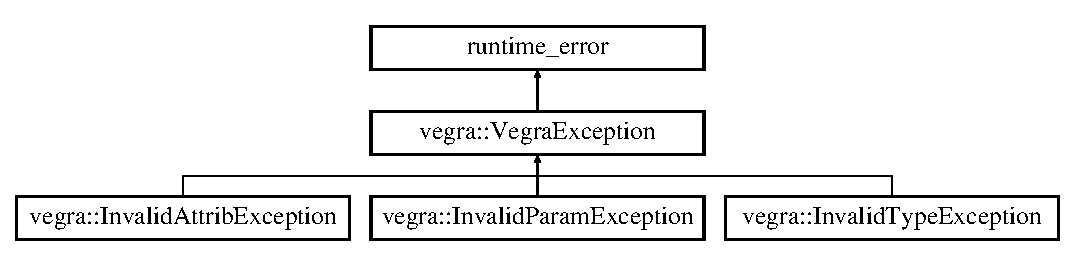
\includegraphics[height=2.994653cm]{structvegra_1_1VegraException}
\end{center}
\end{figure}
\subsection*{Public Member Functions}
\begin{DoxyCompactItemize}
\item 
\mbox{\hyperlink{structvegra_1_1VegraException_a1a020e0b31f096861f1cc79f78c02706}{Vegra\+Exception}} (const std\+::string \&msg)
\end{DoxyCompactItemize}


\subsection{Detailed Description}
Base Exception. 

\subsection{Constructor \& Destructor Documentation}
\mbox{\Hypertarget{structvegra_1_1VegraException_a1a020e0b31f096861f1cc79f78c02706}\label{structvegra_1_1VegraException_a1a020e0b31f096861f1cc79f78c02706}} 
\index{vegra\+::\+Vegra\+Exception@{vegra\+::\+Vegra\+Exception}!Vegra\+Exception@{Vegra\+Exception}}
\index{Vegra\+Exception@{Vegra\+Exception}!vegra\+::\+Vegra\+Exception@{vegra\+::\+Vegra\+Exception}}
\subsubsection{\texorpdfstring{Vegra\+Exception()}{VegraException()}}
{\footnotesize\ttfamily vegra\+::\+Vegra\+Exception\+::\+Vegra\+Exception (\begin{DoxyParamCaption}\item[{const std\+::string \&}]{msg }\end{DoxyParamCaption})\hspace{0.3cm}{\ttfamily [inline]}, {\ttfamily [explicit]}}



The documentation for this struct was generated from the following file\+:\begin{DoxyCompactItemize}
\item 
/home/raghu/\+Development/vegra/include/\mbox{\hyperlink{exception_8h}{exception.\+h}}\end{DoxyCompactItemize}

\chapter{File Documentation}
\hypertarget{attrib_8h}{}\section{/home/raghu/\+Development/vegra/include/attrib.h File Reference}
\label{attrib_8h}\index{/home/raghu/\+Development/vegra/include/attrib.\+h@{/home/raghu/\+Development/vegra/include/attrib.\+h}}
\subsection*{Classes}
\begin{DoxyCompactItemize}
\item 
struct \mbox{\hyperlink{structvegra_1_1Position}{vegra\+::\+Position}}
\item 
struct \mbox{\hyperlink{structvegra_1_1Center}{vegra\+::\+Center}}
\item 
struct \mbox{\hyperlink{structvegra_1_1Radius}{vegra\+::\+Radius}}
\item 
struct \mbox{\hyperlink{structvegra_1_1Size}{vegra\+::\+Size}}
\item 
struct \mbox{\hyperlink{structvegra_1_1Stroke}{vegra\+::\+Stroke}}
\begin{DoxyCompactList}\small\item\em Attribute to outline the element. \end{DoxyCompactList}\item 
struct \mbox{\hyperlink{structvegra_1_1Fill}{vegra\+::\+Fill}}
\begin{DoxyCompactList}\small\item\em Attribute control fill inside the svg element. \end{DoxyCompactList}\end{DoxyCompactItemize}
\subsection*{Namespaces}
\begin{DoxyCompactItemize}
\item 
 \mbox{\hyperlink{namespacevegra}{vegra}}
\begin{DoxyCompactList}\small\item\em namespace vegra \end{DoxyCompactList}\end{DoxyCompactItemize}
\subsection*{Enumerations}
\begin{DoxyCompactItemize}
\item 
enum \mbox{\hyperlink{namespacevegra_a342c4e8c946c4f729d694257d1ed876b}{vegra\+::\+Font\+Family}} \{ \newline
\mbox{\hyperlink{namespacevegra_a342c4e8c946c4f729d694257d1ed876ba6fbda3a3567da6d01bc9da915e91d702}{vegra\+::\+Font\+Family\+::\+Arial}}, 
\mbox{\hyperlink{namespacevegra_a342c4e8c946c4f729d694257d1ed876ba9b846c60f2b2d24b350f55077e4dd894}{vegra\+::\+Font\+Family\+::\+Helvetica}}, 
\mbox{\hyperlink{namespacevegra_a342c4e8c946c4f729d694257d1ed876babf103d5f351643099afbb4cc28ba9946}{vegra\+::\+Font\+Family\+::\+Times\+New\+Roman}}, 
\mbox{\hyperlink{namespacevegra_a342c4e8c946c4f729d694257d1ed876bab3ac111fd7521343dd1a3fabce8279c2}{vegra\+::\+Font\+Family\+::\+Times}}, 
\newline
\mbox{\hyperlink{namespacevegra_a342c4e8c946c4f729d694257d1ed876ba96e248eff9ac321d7f79d2cdb142f49c}{vegra\+::\+Font\+Family\+::\+Courier\+New}}, 
\mbox{\hyperlink{namespacevegra_a342c4e8c946c4f729d694257d1ed876ba5055d1a4444c630d6839f48ab48aef91}{vegra\+::\+Font\+Family\+::\+Courier}}, 
\mbox{\hyperlink{namespacevegra_a342c4e8c946c4f729d694257d1ed876ba207c321933d5e7273bf3defb9eca01af}{vegra\+::\+Font\+Family\+::\+Verdana}}, 
\mbox{\hyperlink{namespacevegra_a342c4e8c946c4f729d694257d1ed876baeada819634d0164c6a7547bdcc405033}{vegra\+::\+Font\+Family\+::\+Georgia}}, 
\newline
\mbox{\hyperlink{namespacevegra_a342c4e8c946c4f729d694257d1ed876ba3dbbdc472c939827d1aa5e8c51f7aa85}{vegra\+::\+Font\+Family\+::\+Palatino}}, 
\mbox{\hyperlink{namespacevegra_a342c4e8c946c4f729d694257d1ed876ba96a7872564f8ba8cb1d2975a13bde360}{vegra\+::\+Font\+Family\+::\+Garamond}}, 
\mbox{\hyperlink{namespacevegra_a342c4e8c946c4f729d694257d1ed876ba3919198dda599c06f83ad77a698598ce}{vegra\+::\+Font\+Family\+::\+Bookman}}, 
\mbox{\hyperlink{namespacevegra_a342c4e8c946c4f729d694257d1ed876ba7162619c10d2933c5dd5afa5c8012b8b}{vegra\+::\+Font\+Family\+::\+Comic\+Sans\+MS}}, 
\newline
\mbox{\hyperlink{namespacevegra_a342c4e8c946c4f729d694257d1ed876ba59b2d6b423cfc293af6522c3d2806199}{vegra\+::\+Font\+Family\+::\+Trebuchet\+MS}}, 
\mbox{\hyperlink{namespacevegra_a342c4e8c946c4f729d694257d1ed876ba90c2472318c987dd8c65516ce3b7a614}{vegra\+::\+Font\+Family\+::\+Arial\+Black}}, 
\mbox{\hyperlink{namespacevegra_a342c4e8c946c4f729d694257d1ed876ba21f59b54f62b5b8b4bc0f63f0f617fc1}{vegra\+::\+Font\+Family\+::\+Impact}}
 \}
\begin{DoxyCompactList}\small\item\em Enumeration of Web Safe Font Family. \end{DoxyCompactList}\end{DoxyCompactItemize}
\subsection*{Functions}
\begin{DoxyCompactItemize}
\item 
std\+::string \mbox{\hyperlink{namespacevegra_a776f7d3c50693931a482a34284b43ede}{vegra\+::to\+\_\+string}} (const \mbox{\hyperlink{namespacevegra_a342c4e8c946c4f729d694257d1ed876b}{vegra\+::\+Font\+Family}} \&font\+Family)
\begin{DoxyCompactList}\small\item\em Function to convert given Font Family from enum type to string type. \end{DoxyCompactList}\end{DoxyCompactItemize}

\hypertarget{circle_8h}{}\section{/home/raghu/\+Development/vegra/include/circle.h File Reference}
\label{circle_8h}\index{/home/raghu/\+Development/vegra/include/circle.\+h@{/home/raghu/\+Development/vegra/include/circle.\+h}}
\subsection*{Classes}
\begin{DoxyCompactItemize}
\item 
struct \mbox{\hyperlink{structvegra_1_1Circle}{vegra\+::\+Circle}}
\end{DoxyCompactItemize}
\subsection*{Namespaces}
\begin{DoxyCompactItemize}
\item 
 \mbox{\hyperlink{namespacevegra}{vegra}}
\begin{DoxyCompactList}\small\item\em namespace vegra \end{DoxyCompactList}\end{DoxyCompactItemize}
\subsection*{Typedefs}
\begin{DoxyCompactItemize}
\item 
using \mbox{\hyperlink{namespacevegra_a2722f5eceb74f65746a02a57b71d125e}{vegra\+::\+S\+V\+G\+Element\+List}} = std\+::vector$<$ \mbox{\hyperlink{structvegra_1_1SVGElement}{vegra\+::\+S\+V\+G\+Element}} $\ast$ $>$
\end{DoxyCompactItemize}

\hypertarget{constants_8h}{}\section{/home/raghu/\+Development/vegra/include/constants.h File Reference}
\label{constants_8h}\index{/home/raghu/\+Development/vegra/include/constants.\+h@{/home/raghu/\+Development/vegra/include/constants.\+h}}
\subsection*{Namespaces}
\begin{DoxyCompactItemize}
\item 
 \mbox{\hyperlink{namespacevegra}{vegra}}
\begin{DoxyCompactList}\small\item\em namespace vegra \end{DoxyCompactList}\item 
 \mbox{\hyperlink{namespacevegra_1_1attr}{vegra\+::attr}}
\end{DoxyCompactItemize}
\subsection*{Variables}
\begin{DoxyCompactItemize}
\item 
const std\+::string \mbox{\hyperlink{namespacevegra_a490ca2f98836fa22a92f9e141cc7ab1e}{vegra\+::\+S\+P\+A\+CE}} = \char`\"{} \char`\"{}
\item 
const std\+::string \mbox{\hyperlink{namespacevegra_adc1a2a72f90b97032bad20408a31dfb5}{vegra\+::\+E\+Q\+U\+A\+LS}} = \char`\"{}=\char`\"{}
\item 
const std\+::string \mbox{\hyperlink{namespacevegra_a6497d9c2bf3f1c7851bb59fd5af18ec2}{vegra\+::\+O\+T\+AG}} = \char`\"{}$<$\char`\"{}
\item 
const std\+::string \mbox{\hyperlink{namespacevegra_a9acf42016e6b9b201f6894fc1816240d}{vegra\+::\+C\+T\+AG}} = \char`\"{}$>$\char`\"{}
\item 
const std\+::string \mbox{\hyperlink{namespacevegra_abecfb0297d777200fecd622c806fd4a2}{vegra\+::\+F\+S\+L\+A\+SH}} = \char`\"{}/\char`\"{}
\item 
const std\+::string \mbox{\hyperlink{namespacevegra_ab1b1502dc2e3ca49f55d674d8b669301}{vegra\+::\+D\+Q\+U\+O\+TE}} = \char`\"{}\textbackslash{}\char`\"{}\char`\"{}
\item 
const std\+::string \mbox{\hyperlink{namespacevegra_aa1c954f0d9675c3c30a64de7b8bafdc2}{vegra\+::\+C\+O\+M\+MA}} = \char`\"{},\char`\"{}
\item 
const std\+::string \mbox{\hyperlink{namespacevegra_a85bf5beb5ac2df54e14ee7cd075c17e7}{vegra\+::\+E\+X\+T\+E\+N\+S\+I\+ON}} = \char`\"{}.svg\char`\"{}
\item 
const std\+::string \mbox{\hyperlink{namespacevegra_1_1attr_aad742b5d9766de5e8de120f9ec2d606c}{vegra\+::attr\+::x}} = \char`\"{}x\char`\"{}
\item 
const std\+::string \mbox{\hyperlink{namespacevegra_1_1attr_aa7b0fe91ac9ac2d7ef82a96fbc045cef}{vegra\+::attr\+::y}} = \char`\"{}y\char`\"{}
\item 
const std\+::string \mbox{\hyperlink{namespacevegra_1_1attr_a2b00c1ce5fbfd6f287f04c82436cde36}{vegra\+::attr\+::cx}} = \char`\"{}cx\char`\"{}
\begin{DoxyCompactList}\small\item\em P\+O\+SN OF C\+E\+N\+T\+ER F\+OR C\+I\+R\+C\+U\+L\+AR S\+H\+A\+P\+ES. \end{DoxyCompactList}\item 
const std\+::string \mbox{\hyperlink{namespacevegra_1_1attr_aa7ba703fc5e3503eebf09e612e0acfbe}{vegra\+::attr\+::cy}} = \char`\"{}cy\char`\"{}
\item 
const std\+::string \mbox{\hyperlink{namespacevegra_1_1attr_a381876de77425abfb3621bf6f1988ada}{vegra\+::attr\+::height}} = \char`\"{}height\char`\"{}
\begin{DoxyCompactList}\small\item\em S\+I\+ZE. \end{DoxyCompactList}\item 
const std\+::string \mbox{\hyperlink{namespacevegra_1_1attr_ad16d3f19ee0c2bc1624c97839c99dad6}{vegra\+::attr\+::width}} = \char`\"{}width\char`\"{}
\item 
const std\+::string \mbox{\hyperlink{namespacevegra_1_1attr_abfc8a39fd1a64cddfd2e0c599154364b}{vegra\+::attr\+::radius}} = \char`\"{}r\char`\"{}
\begin{DoxyCompactList}\small\item\em R\+A\+D\+I\+US. \end{DoxyCompactList}\item 
const std\+::string \mbox{\hyperlink{namespacevegra_1_1attr_a239f7c243700210a4a201335a34bcef9}{vegra\+::attr\+::fill}} = \char`\"{}fill\char`\"{}
\begin{DoxyCompactList}\small\item\em F\+I\+LL. \end{DoxyCompactList}\item 
const std\+::string \mbox{\hyperlink{namespacevegra_1_1attr_a9d77466dca979b9cebbcac29c4a86c28}{vegra\+::attr\+::fill\+\_\+opacity}} = \char`\"{}fill-\/opacity\char`\"{}
\item 
const std\+::string \mbox{\hyperlink{namespacevegra_1_1attr_a547c61d63fa7cd98b099cfddda3e900f}{vegra\+::attr\+::stroke}} = \char`\"{}stroke\char`\"{}
\begin{DoxyCompactList}\small\item\em S\+T\+R\+O\+KE. \end{DoxyCompactList}\item 
const std\+::string \mbox{\hyperlink{namespacevegra_1_1attr_afaba5780f0fd064b750037b66af7d6a0}{vegra\+::attr\+::stroke\+\_\+width}} = \char`\"{}stroke-\/width\char`\"{}
\item 
const std\+::string \mbox{\hyperlink{namespacevegra_1_1attr_a38bbcd92795d4200270ffb0cc654b396}{vegra\+::attr\+::stroke\+\_\+opacity}} = \char`\"{}stroke-\/opacity\char`\"{}
\item 
const std\+::string \mbox{\hyperlink{namespacevegra_1_1attr_a19195ef7c83cf394bf879490c05ff279}{vegra\+::attr\+::stroke\+\_\+dasharray}} = \char`\"{}stroke-\/dasharray\char`\"{}
\item 
const std\+::string \mbox{\hyperlink{namespacevegra_1_1attr_a58600e14ff5c6f05ce98fb91bbd0ecb3}{vegra\+::attr\+::stroke\+\_\+dashoffset}} = \char`\"{}stroke-\/dashoffset\char`\"{}
\item 
const std\+::string \mbox{\hyperlink{namespacevegra_1_1attr_a01f922256bd62abf2554d5438fda3b62}{vegra\+::attr\+::stroke\+\_\+linecap}} = \char`\"{}stroke-\/linecap\char`\"{}
\end{DoxyCompactItemize}

\hypertarget{elements_8h}{}\section{/home/raghu/\+Development/vegra/include/elements.h File Reference}
\label{elements_8h}\index{/home/raghu/\+Development/vegra/include/elements.\+h@{/home/raghu/\+Development/vegra/include/elements.\+h}}
{\ttfamily \#include \char`\"{}constants.\+h\char`\"{}}\newline
\subsection*{Classes}
\begin{DoxyCompactItemize}
\item 
struct \mbox{\hyperlink{structvegra_1_1SVGElement}{vegra\+::\+S\+V\+G\+Element}}
\begin{DoxyCompactList}\small\item\em \mbox{\hyperlink{structvegra_1_1SVGElement}{S\+V\+G\+Element}} -\/ Parent class for all svg elements. \end{DoxyCompactList}\end{DoxyCompactItemize}
\subsection*{Namespaces}
\begin{DoxyCompactItemize}
\item 
 \mbox{\hyperlink{namespacevegra}{vegra}}
\begin{DoxyCompactList}\small\item\em namespace vegra \end{DoxyCompactList}\end{DoxyCompactItemize}
\subsection*{Functions}
\begin{DoxyCompactItemize}
\item 
std\+::string \mbox{\hyperlink{namespacevegra_a35980cba2dab0fb1d1e3154dfa23cbfc}{vegra\+::\+Q\+U\+O\+TE}} (std\+::string value)
\begin{DoxyCompactList}\small\item\em utility wrapper functions \end{DoxyCompactList}\item 
std\+::string \mbox{\hyperlink{namespacevegra_ad53777752123522d1807f483fa01c0a5}{vegra\+::\+W\+R\+AP}} (std\+::string value)
\begin{DoxyCompactList}\small\item\em T\+O\+D\+O(raghu)\+: Change to std\+::quoted if compiler is c++14 compliant. \end{DoxyCompactList}\item 
std\+::string \mbox{\hyperlink{namespacevegra_a46b18aa974bf220f63e7d00163eb549a}{vegra\+::\+M\+U\+L\+T\+I\+\_\+\+W\+R\+AP}} (std\+::string tagname, std\+::string self, S\+V\+G\+Element\+List elements)
\begin{DoxyCompactList}\small\item\em Wrap element with opening and closing tag, only with attributes. \end{DoxyCompactList}\item 
std\+::string \mbox{\hyperlink{namespacevegra_a4893502d3540c9e206e49072ffaa4316}{vegra\+::\+A\+S\+S\+I\+GN}} (std\+::string attr, std\+::string value)
\item 
std\+::string \mbox{\hyperlink{namespacevegra_ac0412cf8d762772ec0857239d5d47eb3}{vegra\+::\+S\+TR}} (int value)
\begin{DoxyCompactList}\small\item\em convert all non string values to string type \end{DoxyCompactList}\item 
std\+::string \mbox{\hyperlink{namespacevegra_a5365ef337b0b536116d63a2352fd903d}{vegra\+::\+S\+TR}} (std\+::pair$<$ int, int $>$ value)
\end{DoxyCompactItemize}

\hypertarget{exception_8h}{}\section{/home/raghu/\+Development/vegra/include/exception.h File Reference}
\label{exception_8h}\index{/home/raghu/\+Development/vegra/include/exception.\+h@{/home/raghu/\+Development/vegra/include/exception.\+h}}
\subsection*{Classes}
\begin{DoxyCompactItemize}
\item 
struct \mbox{\hyperlink{structvegra_1_1VegraException}{vegra\+::\+Vegra\+Exception}}
\begin{DoxyCompactList}\small\item\em Base Exception. \end{DoxyCompactList}\item 
struct \mbox{\hyperlink{structvegra_1_1InvalidAttribException}{vegra\+::\+Invalid\+Attrib\+Exception}}
\begin{DoxyCompactList}\small\item\em Invalid attrib exception -\/ Throw when invalid attribute is passed to a function. \end{DoxyCompactList}\item 
struct \mbox{\hyperlink{structvegra_1_1InvalidParamException}{vegra\+::\+Invalid\+Param\+Exception}}
\item 
struct \mbox{\hyperlink{structvegra_1_1InvalidTypeException}{vegra\+::\+Invalid\+Type\+Exception}}
\begin{DoxyCompactList}\small\item\em Invalid Type Exception -\/ Throw when a non svg type is passed. \end{DoxyCompactList}\end{DoxyCompactItemize}
\subsection*{Namespaces}
\begin{DoxyCompactItemize}
\item 
 \mbox{\hyperlink{namespacevegra}{vegra}}
\begin{DoxyCompactList}\small\item\em namespace vegra \end{DoxyCompactList}\end{DoxyCompactItemize}

\hypertarget{rect_8h}{}\section{/home/raghu/\+Development/vegra/include/rect.h File Reference}
\label{rect_8h}\index{/home/raghu/\+Development/vegra/include/rect.\+h@{/home/raghu/\+Development/vegra/include/rect.\+h}}
\subsection*{Classes}
\begin{DoxyCompactItemize}
\item 
struct \mbox{\hyperlink{structvegra_1_1Rect}{vegra\+::\+Rect}}
\end{DoxyCompactItemize}
\subsection*{Namespaces}
\begin{DoxyCompactItemize}
\item 
 \mbox{\hyperlink{namespacevegra}{vegra}}
\begin{DoxyCompactList}\small\item\em namespace vegra \end{DoxyCompactList}\end{DoxyCompactItemize}

\hypertarget{vegra_8h}{}\section{/home/raghu/\+Development/vegra/include/vegra.h File Reference}
\label{vegra_8h}\index{/home/raghu/\+Development/vegra/include/vegra.\+h@{/home/raghu/\+Development/vegra/include/vegra.\+h}}
{\ttfamily \#include $<$type\+\_\+traits$>$}\newline
{\ttfamily \#include $<$string$>$}\newline
{\ttfamily \#include $<$memory$>$}\newline
{\ttfamily \#include $<$map$>$}\newline
{\ttfamily \#include $<$algorithm$>$}\newline
{\ttfamily \#include $<$vector$>$}\newline
{\ttfamily \#include $<$fstream$>$}\newline
{\ttfamily \#include $<$iomanip$>$}\newline
{\ttfamily \#include \char`\"{}constants.\+h\char`\"{}}\newline
{\ttfamily \#include \char`\"{}exception.\+h\char`\"{}}\newline
{\ttfamily \#include \char`\"{}attrib.\+h\char`\"{}}\newline
{\ttfamily \#include \char`\"{}elements.\+h\char`\"{}}\newline
{\ttfamily \#include \char`\"{}rect.\+h\char`\"{}}\newline
{\ttfamily \#include \char`\"{}circle.\+h\char`\"{}}\newline
\subsection*{Classes}
\begin{DoxyCompactItemize}
\item 
struct \mbox{\hyperlink{structvegra_1_1SVG}{vegra\+::\+S\+VG}}
\begin{DoxyCompactList}\small\item\em \mbox{\hyperlink{structvegra_1_1SVG}{S\+VG}} element. \end{DoxyCompactList}\end{DoxyCompactItemize}
\subsection*{Namespaces}
\begin{DoxyCompactItemize}
\item 
 \mbox{\hyperlink{namespacevegra}{vegra}}
\begin{DoxyCompactList}\small\item\em namespace vegra \end{DoxyCompactList}\end{DoxyCompactItemize}

%--- End generated contents ---

% Index
\backmatter
\newpage
\phantomsection
\clearemptydoublepage
\addcontentsline{toc}{chapter}{\indexname}
\printindex

\end{document}
